\documentclass[aps,rmp,reprint,amsmath,amssymb,longbibliography,twocolumn,floatfix]{revtex4-1}

% Include the configuration file
\usepackage{bm}
\usepackage{graphicx}
\usepackage{epstopdf}
\usepackage{wrapfig}
\usepackage{array} 
\usepackage{listings}
\usepackage[para,online,flushleft]{threeparttablex}
\usepackage{booktabs,dcolumn}
\usepackage{color}
\usepackage{comment}
 
\usepackage{textpos}
\usepackage{booktabs}
\usepackage{multirow,bigdelim}
\usepackage{float}
\usepackage{tikz}
\usepackage{dsfont}
% \usepackage{subfigure}
\usepackage{float}
% \usepackage{caption}
% \usepackage{subcaption}
\usepackage{subfig}
\usepackage{pgfplots}

\pgfplotsset{width=\textwidth*0.5, height=\textwidth/3*0.5,compat=1.18}

\usepackage[super]{nth}

\usepackage{upgreek} %upalpha in Saxena2021 Reference

\usepackage[utf8]{inputenc}
\usepackage{hyperref}
\hypersetup{breaklinks=true,colorlinks=true,linkcolor=blue,citecolor=blue,filecolor=magenta,urlcolor=blue}

\usepackage{lipsum}


\usepackage{xcolor}
%\newcommand{\contrib}[1]{\textcolor{red}{#1}}
%\newcommand{\comment}[1]{\textcolor{blue}{#1}}

%\newcommand{\WN}[1]{{\color{red} #1}}

\makeatletter
\def\@bibdataout@aps{%
\immediate\write\@bibdataout{%
@CONTROL{%
apsrev41Control%
\longbibliography@sw{%
    ,author="08",editor="1",pages="1",title="0",year="1"%
    }{%
    ,author="08",editor="1",pages="1",title="",year="1"%
    }%
  }%
}%
\if@filesw \immediate \write \@auxout {\string \citation {apsrev41Control}}\fi
}
\makeatother

\DeclareMathOperator*{\argmax}{arg\,max}
\DeclareMathOperator*{\argmin}{arg\,min}
\DeclareMathOperator{\MSE}{MSE}
\DeclareMathOperator*{\compfunc}{\bigcirc}


%\usepackage[left]{lineno}
%\linenumbers

\begin{document}
% \pagenumbering{gobble} 

\title{UX-PINNs: A User-friendly Implementation of Extended Physics-Informed Neural Networks}
\title{JAXPINNs: Extended Physics-Informed Neural Networks implemented with JAX.}

\author{Femtehjell, Winsvold, Steeneveldt, Johannessen and Hu}
% \affiliation{Department of Mathematics, University of Oslo, N-0316 Oslo, Norway}
\date{March 2024}
\affiliation{Department of Mathematics}


\begin{abstract}
\lipsum[1-1] 
\end{abstract}

\maketitle

\tableofcontents

\section{Introduction}
The resolution of Partial Differential Equations (PDEs) underpins % pun intended
many scientific and engineering challenges, notably exemplified by the Navier-Stokes equations governing fluid dynamics. Traditional numerical methods struggle with the computational burdens of modeling many different physical phenomena within a unified framework. In response, Physics-Informed Neural Networks (PINNs) have emerged as a promising alternative, leveraging deep learning to approximate solutions of PDEs while inherently encoding physical laws.

A typical Neural Network is trained through measuring how well the model is able to predict a set of labeled data, often through the Mean Squared Error (MSE). The cost function underpinning the network can then simply be
\begin{equation}
    \mathcal{C}(\boldsymbol{\theta}; \boldsymbol{x}, \boldsymbol{y}) = \lVert \boldsymbol{y} - \mathcal{N}_{\boldsymbol{\theta}}(\boldsymbol{x}) \rVert_2,
\end{equation}
where $\boldsymbol{y}$ are the target values, $\mathcal{N}_\theta(\cdot)$ is the realization of the network given the parameters $\boldsymbol{\theta}$ and the corresponding input values $\boldsymbol{x}$. 
A PINN integrates physical constraints directly into its loss function, effectively guiding the neural network to respect the underlying physics of the problem. This can often remove the requirement of having labeled data for training, which can be a computationally expensive aspect of solving PDEs in and of itself.

\begin{comment}
PINNs build upon this idea, extending the cost function in order to integrate the physical laws governing the problem.
Consider a PDE on the domain $\Omega$ of the form
\begin{equation*}
    \mathcal{L}u^* = f \in \Omega \quad \text{and} \quad u^* = g \in \partial \Omega,
\end{equation*}
where $\mathcal{L}$ is the differential operator characterizing the PDE, $u^*$ is the unknown solution, and $\delta \Omega$ is the boundary. We approximate $u^*$ with $\mathcal{N}_\theta$ by appending
\begin{equation*}
    
\end{equation*}
\end{comment}


However, solving the Navier-Stokes equation with PINNs is costly. So to mitigate our use of computational resources we propose to use the extension of PINNs (XPINNs) through domain decomposition, as presented in \textcite{Jagtap2020ExtendedPN}, which segments the problem domain into simpler, more homogeneous subdomains. This approach enhances computational efficiency and model accuracy, but also introduces challenges in maintaining continuity and physical fidelity across interfaces.

By decomposing the computational domain, we aim to reduce the overall complexity, enabling more efficient training and higher-fidelity solutions, especially in scenarios with multifaceted fluid behaviors. We introduce *methodologies* [TODO: hvilke?] to seamlessly integrate subdomain solutions, ensuring consistent flow properties and energy conservation across interfaces. 

To tackle the computational cost of computing the Navier-Stokes equations and the domain decomposition approach, numerical differentiation is one of the most important components. We therefore incorporate FLAX, a versatile and efficient neural network library for JAX, to enhance our numerical differentiation processes. By leveraging FLAX's capabilities, we aim to streamline the computation of gradients and higher-order derivatives required for the physics-informed loss functions. This is useful for the Navier-Stokes equations, where efficient computation of fluid dynamics variables—such as velocity gradients and pressure differentials is important. FLAX's integration into our XPINNs framework allows for efficient backpropagation, enabling the automatic adjustment of neural network weights to minimize the loss function that encodes both the PDE constraints and the boundary conditions. Another benefit is FLAX's compatibility with JAX's just-in-time compilation and automatic vectorization features which will significantly enhance the computational efficiency of our models, particularly in the parallel processing of multiple subdomains.

Our contributions are twofold: First, we develop a robust framework for XPINNs tailored to the Navier-Stokes equations, incorporating domain decomposition techniques to capture the dynamics of fluid flow. Second, we implement novel loss function configurations and inter-network communication protocols to ensure physical accuracy and computational efficiency across decomposed domains.

Through this work, we [TODO: hype]\label{sec:introduction}

\section{Theory}
\subsection{Neural Networks}
Neural networks are built upon a simplified understanding of how the neurons in the brain function, wherein electrical impulses are passed in a chain reaction throughout the brain.
Feed-forward neural networks typically model this by passing an input through a composition of linear transformations and non-linear activation functions.
In a so-called \textit{feed-forward pass}, the input values $\boldsymbol{x} \in \mathbb{R}^{N_0}$ are sent to each neuron in the next layer, multiplied by a predetermined weight along the way with a value added called the bias $\boldsymbol{b} \in \mathbb{R}^{N_1}$.
We represent this through the function $\mathcal{A} : \mathbb{R}^{N_{i-1}} \to \mathbb{R}^{N_{i}}$ defined by
\begin{equation}\label{eq:A_func}
    \mathcal{A}_i(\boldsymbol{x}) = W_i \boldsymbol{x} + \boldsymbol{b}_i,
\end{equation}
where $W \in \mathbb{R}^{N_i \times N_{i-1}}$ is the weight matrix, where the $N_i$ is the number of neurons in layer $i$.
The resulting values are denoted $\boldsymbol{z}^i$.

The result of this is then passed through an activation function $\sigma_i : \mathbb{R} \to \mathbb{R}$, which we apply element-wise by $\boldsymbol{a}^i_j = \sigma_i (\boldsymbol{z}^i_j)$.
To simplify notation, we simply notate this as $\boldsymbol{a}^i = \sigma_i(\boldsymbol{z}^i)$.
This continues throughout each layer, culminating in the output layer, which in our case will simply have a the identity function as its activation function.
This process is illustrated in \autoref{fig:SimpleFFNN}.

\begin{figure}[h]
\centering
\def\layersep{2.5cm}
\def\nodeinlayersep{1.2cm}
\begin{tikzpicture}[shorten >=1pt,->,draw=black!50, node distance=\layersep]
    \tikzstyle{every pin edge}=[<-,shorten <=1pt]
    \tikzstyle{neuron}=[circle, fill=black!25,minimum size=20pt,inner sep=0pt]
    \tikzstyle{input neuron}=[neuron, fill=red!50];
    \tikzstyle{output neuron}=[neuron, fill=orange!50];
    \tikzstyle{hidden neuron}=[neuron, fill=blue!50, minimum size=20pt];
    \tikzstyle{hidden neuron2}=[neuron, fill=blue!50, minimum size=20pt];

    \foreach \name / \y in {0,...,2}
        \node[input neuron] (I-\name) at (0,-\y) {};

    \foreach \name / \y in {0,...,3}
        \path[yshift=0.5cm]
            node[hidden neuron] (H1-\name) at (\layersep,-\y cm) {};

    \foreach \name / \y in {0,...,3}
        \path[yshift=0.5cm]
            node[hidden neuron2] (H2-\name) at (2*\layersep,-\y cm) {};    

    \foreach \name / \y in {0,...,1}
        % \node[output neuron,pin={[pun edge={->}]right:Output \#\y}, right of=H2-2] (O-\name) at (3*\layersep, -\y cm) {};
        \path[yshift=-0.5cm]
            node[output neuron] (O-\name) at (3*\layersep, -\y cm) {};


    \foreach \source in {0,...,2}
        \foreach \dest in {0,...,3}
            \path (I-\source) edge (H1-\dest);

    \foreach \source in {0,...,3}
        \foreach \dest in {0,...,3}
            \path (H1-\source) edge (H2-\dest);

    \foreach \source in {0,...,3}
        \foreach \dest in {0,...,1}
            \path (H2-\source) edge (O-\dest);
\end{tikzpicture}
\caption{Illustration of a fully connected feed-forward neural network with an input layer (teal), two hidden layers (purple) and an output layer (beige).}
\label{fig:SimpleFFNN}
\end{figure}

Let $\boldsymbol{\theta} = \{ W_i, \boldsymbol{b}_i \}_{i = 1}^L$ represent the trainable parameters of the network in the parameter space $\mathcal{V}$, and $\mathcal{N}_{\boldsymbol{\theta}} : \mathbb{R}^{N_0} \to \mathbb{R}^{N_L}$ denote the realization of a neural network with $L$ layers, defined through the composition
\begin{equation}\label{eq:NNreal}
\begin{split}
    \mathcal{N}_{\boldsymbol{\theta}} &= \sigma_L \circ \mathcal{A}_L \circ \sigma_{L-1} \circ \ldots \circ \sigma_{1} \circ \mathcal{A}_1 \\
    &= \compfunc_{i = 1}^L \sigma_i \circ \mathcal{A}_i.
\end{split}
\end{equation}
We call the parameters trainable, as we typically initialize them to random values, \textit{training} them through optimization with the help of the backpropagation algorithm.
We do this by measuring how well our model is able to predict a set of values with a cost function $\mathcal{C}$, which often gives the problem the form of finding
\begin{equation}\label{eq:argmintheta}
    \hat{\boldsymbol{\theta}} = \argmin_{\boldsymbol{\theta} \in \mathcal{V}} \mathcal{C} \left( \mathcal{N}_{\boldsymbol{\theta}}, \boldsymbol{x}, \boldsymbol{\hat{y}} \right),
\end{equation}
where $\boldsymbol{\hat{y}} \in \mathbb{R}^{N_L}$ are a set of target values.

A typical choice of $\mathcal{C}$ in a regression problem is the Mean Squared Error (MSE), defined by
\begin{equation}
    \mathcal{C}(\mathcal{N}_\theta, \boldsymbol{x}, \boldsymbol{y}) = \frac{1}{n} \lVert \mathcal{N}_\theta(\boldsymbol{x}) - \boldsymbol{y} \rVert_2^2.
\end{equation}
One of the main benefits of this measure is its ease of differentiation, lightening the computational load of training the network.

Through the Universal Approximation theorem, first proven by \textcite{Cybenko1989ApproximationBS} and since extended, neural networks have a proven capacity to approximate any given function.
It does not state however how one is to find the architecture and parameters which solve a given problem.
The theorem does however guarantee the validity of at least attempting to utilize neural networks in a number of fields.

\subsection{Partial Differential Equations}
A Partial Differential Equation (PDE) is defined to be an equation containing a function with at least two different variables, as well as some degree of partial derivatives to these variables.
PDEs are ubiquitous in describing the properties, behavior, and evolution of physical systems.

An important concept when discussing PDEs is differential operators.
A differential operator is defined as a function performing some sort of differentiation on the function it is applied to.
It is indeed a function from a function space $\mathcal{F}_1$ to another function space $\mathcal{F}_2$.
In the case of a function of $n$ variables $u(x_1, x_2, \ldots , x_n)$ the usual differential operator is defined as 
\begin{equation*}
    D^\alpha u = \frac{\partial u^{|\alpha|}}{\partial x_1^{\alpha_1} \partial x_2^{\alpha_2} \cdots \partial x_n^{\alpha_n}},
\end{equation*}
where $|\alpha| = \alpha_1 + \alpha_2 + \ldots + \alpha_n$.
When considering a function $u(x,y)$, we will denote $\frac{\partial u}{\partial x}$ as $u_x$, $\frac{\partial^2 u}{\partial x^2}$ as $u_{xx}$, and so on.
We will when discussing general PDEs denote the differential operator characterizing the PDE by $\mathcal{L}$.

An example of a PDE is Poisson's equation, which is characterized by
\begin{equation*}
    u_{xx} + u_{yy} = f \text{ on }\Omega,
\end{equation*}
where the residual $f$ is independent of $u$, on the domain $\Omega \in \mathbb{R}^d$, where $d$ is the number of dimensions.
In the 2D case, we have $\mathcal{L}u = u_{xx} + u_{yy}$, so that the equation can be denoted succinctly as $\mathcal{L}u = f$.

We will also come across the differential operator $\nabla$.
For a problem in three physical dimensions, $\nabla$ is defined as $\nabla = \frac{\partial}{\partial x}\boldsymbol{x} + \frac{\partial}{\partial y}\boldsymbol{y} + \frac{\partial}{\partial z}\boldsymbol{z}$, where $\boldsymbol{x},\boldsymbol{y},\boldsymbol{z}$ are the three-dimensional Euclidean unit vectors.

When considering time-dependent PDEs for physical problems, we frequently require initial and boundary conditions.
Initial conditions are conditions for values at $t=0$, and boundary conditions are conditions on the physical boundaries of the problem.
Thus, both conditions are defined on the boundary $\partial\Omega$ of our spatial-temporal domain, and we treat them similarly.
In this paper we encounter Dirichlet-type boundary conditions, where the value of the function on the boundary is given.
We return to the Poisson equation as an example;
we have for the function $u(x,y)$, $(x,y) \in [0,1]\times [0,1]$, the boundary conditions $u(0,y)=u(1,y)=u(x,0)=u(x,1) = 0$.
Neumann boundary conditions are also ubiquitous. This is when the boundary conditions determine the first order derivative in the direction normal to the boundary. 

To capture these boundary conditions, we introduce a boundary value operator $\mathcal B$ such that we can write $\mathcal B u = g$ on $\partial \Omega$ for all our boundary conditions, for some function $g$ on the boundary $\partial\Omega$.
Given the PDE operator $\mathcal L$ and the boundary value operator $\mathcal B$, we present the general form of a PDE as
\begin{equation}
\begin{cases}
    \mathcal{L}u = f &\text{in } \Omega,\\
    \mathcal{B}u = g &\text{in } \partial\Omega.
\end{cases}
\label{eq:PDE}
\end{equation}

\subsection{Physics-Informed Neural Networks}
Physics-Informed Neural Networks (PINNs) incorporate the inherent physical constraints of a problem directly into the network.
One such way is to bake in the PDE conditions of a problem directly into the loss function of the network \cite{RAISSI2019686}.
In doing so, we coerce the network into predicting results which adhere to the inherent physical laws.
In this way, we reduce the need for labeled data, and are able to be more confident in the predictions of our network.
Our neural network $\mathcal{N}_{\boldsymbol{\theta}}$ can then be regarded as an approximation of the hidden function $u$, denoting it as $u^*$.

We then measure the loss through
\begin{equation}\label{eq:PINNMSE}
    \MSE = \MSE_d + \MSE_0 + \MSE_u + \MSE_f,
\end{equation}
where
\begin{equation*}
\begin{split}
    \underbrace{\MSE_d}_{\text{data}} &= \frac{w_d}{N_d} \sum_{i = 0}^{N_d} \left( u^*(x_d^i) - u_d^i \right)^2,  \\
    \underbrace{\MSE_0}_{\text{Initial}} &= \frac{w_0}{N_0} \sum_{i = 0}^{N_0} \left( u^*(x_0^i) - u_0^i \right)^2,  \\
    \underbrace{\MSE_u}_{\text{Boundary}} &= \frac{w_u}{N_u} \sum_{i = 0}^{N_u} \left( u^*(x_u^i) - g(x_u^i) \right)^2, \\
    \underbrace{\MSE_f}_{\text{Residual}} &= \frac{w_f}{N_f} \sum_{i = 0}^{N_f} \left( \mathcal{L}u^*(x_f^i) - f(x_f^i) \right)^2.
\end{split}
\end{equation*}
In this case, $(x_d^i,u_d^i)_{i=1}^{N_d}$ is a sample of data, $u_0^i$ is our initial condition, and $N_d,N_0,N_u,N_f$ is the number of data-, initial-, boundary-, and residual points on which the loss is calculated respectively. $w_d,w_0,w_u,w_f$ are the respective weights given to each loss. 
With this baseline, one can extend the loss function through appending more terms, if there are other conditions, such as periodicity, one would like to enforce.
Note that in $\MSE_f$, we are taking the derivative of the network itself with respect to its output.
This is done through the use of automatic differentiation, in much the same way the parameters are optimized, described further in \autoref{sec:autodiff}.

The $\MSE_d$ can also be dropped, leading to unsupervised training.
However, unsupervised PINNs have been documented to be slower than traditional numerical methods for solving PDEs \cite{en16124558}.
Nevertheless, with a framework already set up, the process of setting up a PINN is quite simple, in contrast to developing a numerical algorithm.

The PINN framework therefore presents a simple methodology to incorporating knowledge about the systems we wish to solve into our neural network training. 
Moreover, PINNs also retain the data-based learning from machine learning models, allowing the user to train using existing data. 
This approach has made PINNs particularly suited for inverse problems. Inverse problems involve determining some parameters of our system using data, and are notoriously difficult for traditional methods \cite{Jagtap_2022,garay2023physicsinformed}.

\subsection{Extended Physics-Informed Neural Networks}
Extended Physics-Informed Neural Networks (XPINNs) is a generalized space-time domain decomposition algorithm for PINNs initially proposed in \textcite{Jagtap2020ExtendedPN}.
The key idea is to decompose the domain $\Omega$ into several subdomains $(\Omega_s)_s^N$ such that $\bigcup_{s=1}^{N_\mathrm{sd}}\Omega_s=\Omega$, as illustrated in \autoref{fig:subdomain_comp}.
The domain interfaces are given by $\Omega_i\cap \Omega_j = \partial\Omega_{ij},\, i\neq j$.
Each subdomain is then equipped with its own sub-PINN $u^*_s$, and the training and test points associated with its subdomain.

\begin{figure}[h]
\centering
\begin{tikzpicture}[x=0.75pt,y=0.75pt,yscale=-1,xscale=1]

\coordinate (Top) at (283.69,109.1);
\coordinate (Left) at (215.67,163);
\coordinate (Bottom) at (298.76,211.69);
\coordinate (Middle) at (275.54,163.47);

\fill[purple!40] (Left) .. controls (240.17,154.14) and (260.97,154.24) .. (Middle) .. controls (290.11,172.69) and (297.8,187.76) .. (Bottom) .. controls (274.65,214.78) and (245.16,212.25) .. (232.3,204.34) .. controls (220.65,197.17) and (215.83,179.98) .. (Left) -- cycle;

\fill[orange!20] (Left) .. controls (215.47,142.06) and (222.36,121.44) .. (232.3,120.34) .. controls (240.46,119.43) and (262.42,112.76) .. (Top) .. controls (293.69,127.1) and (300.54,135.47) .. (Middle) .. controls (260.97,154.24) and (240.17,154.14) .. (Left) -- cycle;

\fill[teal!35] (Top) .. controls (309.31,104.7) and (333.94,104.67) .. (332.3,124.34) .. controls (329.3,160.34) and (312.3,154.34) .. (332.3,184.34) .. controls (342.4,199.5) and (323.39,208.53) .. (Bottom) .. controls (297.8,187.76) and (290.11,172.69) .. (Middle) .. controls (300.54,135.47) and (293.69,127.1) .. (Top) -- cycle;

\draw [thick]  (232.3,120.34) .. controls (240.46,119.43) and (262.42,112.76) .. (283.69,109.1) .. controls (309.31,104.7) and (333.94,104.67) .. (332.3,124.34) .. controls (329.3,160.34) and (312.3,154.34) .. (332.3,184.34) .. controls (342.4,199.5) and (323.39,208.53) .. (298.76,211.69) .. controls (274.65,214.78) and (245.16,212.25) .. (232.3,204.34) .. controls (220.65,197.17) and (215.83,179.98) .. (215.67,163) .. controls (215.47,142.06) and (222.36,121.44) .. (232.3,120.34) -- cycle ;
%Curve Lines [id:da968003923864855] 
\draw  [dashed]  (215.67,163) .. controls (240.17,154.14) and (260.97,154.24) .. (275.54,163.47) .. controls (290.11,172.69) and (297.8,187.76) .. (298.76,211.69) ;
%Curve Lines [id:da35316263230503897] 
\draw  [dashed]  (283.69,109.1) .. controls (293.69,127.1) and (300.54,135.47) .. (275.54,163.47) ;

% \node (A) at (Left) {};
% \node [rotate=-25, xshift=-0.5cm] (B) [left of=A] {Interface};
% \draw [thick,->] (B) edge (A);
\node [yshift=0.25cm] (C) at (Top) {$\Omega$};

% Text Node
\draw (244,176.4) node [anchor=north west][inner sep=0.75pt]    {$\Omega _{1}$};
% Text Node
\draw (296,153.4) node [anchor=north west][inner sep=0.75pt]    {$\Omega _{3}$};
% Text Node
\draw (245,126.4) node [anchor=north west][inner sep=0.75pt]    {$\Omega _{2}$};

\end{tikzpicture}
\caption{Domain decomposition of $\Omega$ into three subdomains $\Omega_i$, with dashed lines representing the interfaces $\partial \Omega_{ij}$. Each subdomain is equipped with its own unique PINN. }
\label{fig:subdomain_comp}
\end{figure}

Given such a domain decomposition, we now consider the following XPINN solution to our PDE problems:
\begin{equation}\label{eq:XPINN}
    u^* (x)=\sum_{s=1}^{N_\mathrm{sd}} u_{s}^*(x) \mathds{1}_{\Omega_s}(x),
\end{equation}
where $\mathds{1}_{\Omega_s}(x)$ is the indicator function given by:
\begin{equation}
    \mathds{1}_{\Omega_s}(x)=
    \begin{cases}
        0 &\text{If } x \notin \Omega_s \\
        1 &\text{If } x \in \Omega_s \backslash \text{common interface in } \Omega_s \\
        \frac{1}{S} &\text{If } x \in \text{common interface in } \Omega_s,
    \end{cases}
\end{equation}
where $S$ is the number of subdomains intersecting in the common interface.

A classical problem when applying domain decomposition is ensuring sufficient communication between the different subdomains such that their solutions reflect a global solution.
Ideally, the domain decomposition solution should be ``blind" to the decomposition.
For classical solvers, we frequently introduce \textit{ghost layers} to facilitate the communication between neighboring subdomains. 

However, as PINNs are mesh-independent we do not require ghost layers to communicate between PINNs.
XPINNs instead proposes to amend an additional \textit{interface loss} term $\MSE_I$ to the loss function \eqref{eq:PINNMSE} of each PINN to ensure that the PINNs agree on the subdomain interfaces.
For instance, we might wish to enforce continuity in our solution across an interface.
For a single PINN, we amend the loss function with
\begin{equation}\label{eq:MSE_I}
    \underbrace{\MSE_I}_{\text{Interface}} = \frac{1}{N_I} \sum_{i = 0}^{N_d} \left( u^*(x_I^i) - \{u_I^i\} \right)^2,  \\
\end{equation}
where $\{u_I^i\}$ is the average predicted value at the interface from each PINN, and $N_I$ is the number of points on the interface. 

Like traditional domain decomposition algorithms, XPINNs introduce an intuitive parallelization by separating the domain into several subdomains with their own respective neural network where the subdomain solutions can be computed on independent processors.
Thus, XPINNs might improve the computational efficiency through improved utilization of the processor architecture in a computer.

Moreover, \textcite{Jagtap2020ExtendedPN} argue that XPINNs also introduce architectural flexibility into our problem.
For instance, we might employ a deep network in a subdomain with complex solution, whereas we can apply a shallow network for a subdomain with relatively simple and smooth solutions. 

However, the domain decomposition introduces a tradeoff for generalization.
On the one hand, we can leverage the architectural flexibility of XPINNs to decompose a complex PDE solution into several simple parts, decreasing the problem complexity and boosting generalization.
On the other hand, decomposing leads to each subdomain having access to less training data, which might cause overfitting and worse performance overall.
However, in an unsupervised setting, the computational load can be balanced through introducing more points in a previously lighter subdomain.
For a more rigorous analysis of when XPINNs improve generalization, we refer the reader to \cite{XPINN_generalize}.

Furthermore, the interface conditions also introduce complications to the loss function, changing the loss landscape.
Thus, it is easy to imagine instances where for instance the loss landscapes of interface loss and boundary loss are different, resulting in an optimization dilemma of which condition to prioritize.
Moreover, changing the loss function through interface conditions might also correspond to altering the PDE problem equation.
To the extent of the authors' knowledge, there is not a clear theoretical understanding of how the interface conditions alter the solution to our PDE problem. 

\subsection{Automatic Differentiation}\label{sec:autodiff}
The backpropagation algorithm \cite{Backpropogation1986} forms the backbone of training a neural network.
It is the method described in \eqref{eq:backprop}, wherein we take the derivative of the cost function $\mathcal{C}$ with respect to the parameters $\boldsymbol{\theta}$.

$\mathcal{C}$ is a deeply nested function as it involves the realization of the neural network $\mathcal{N}$.
Differentiating this with respect to each parameter of the network is therefore quite a costly task.

There are in essence three methods for calculating this derivative, namely numerical, symbolic or automatic differentiation.
Numerical differentiation relies on the method of finite differences, through approximations such as
\begin{equation}
    f'(x) = \lim_{h \to 0} \frac{f(x+h) - f(x)}{h} \approx \frac{f(x + h) - f(x)}{h},
\end{equation}
for small $h$.
This method can be quite prone to numerical errors, however in a machine learning context this is not a major concern.
What is concerning however, is the fact that we would need to calculate the derivative with respect to each parameter of the network.
As we are potentially working with a huge amount of parameters, this is not feasible

Symbolic, or algorithmic, differentiation refers to a process much like one you would use when differentiating by hand.
The derivatives of elementary functions are hard coded, such that complex expressions can be differentiated through the chain rule.
The reason we don't utilize this method, is that the expressions have a tendency to grow in size.
Consider as an example the function $f(x) = g(x) \cdot h(x)$,
with derivative $f'(x) = g'(x) h(x) + g(x) h'(x)$.
As a neural network is essentially a deeply nested composite function as described by \eqref{eq:NNreal}, this quickly becomes expensive to compute.

Automatic differentiation tackles this issue through keeping track of which terms are repeated throughout the computation.
Consider an extremely simple neural network, with one input and no hidden layer.
The output $y$ is then simply computed as
\begin{equation}\label{eq:supersimple_NN}
    y = \sigma \left( x \cdot w + b \right),
\end{equation}
for an input $x$, weight $w$, bias $b$, and activation function $\sigma$.
The computational graph associated with this is illustrated in \autoref{fig:forward_compgraph}, with $\alpha, \beta, \gamma, \varepsilon$ representing the intermediate values.

\begin{figure}[h]
\centering
\begin{tikzpicture}[node distance=1cm]
    \node[draw, circle, fill=red!20, label=below:$\alpha$] (multiply) {$\times$};
    \node[draw, circle, fill=blue!20, right of=multiply, label=below:$\beta$] (addition) {$+$};
    \node[draw, circle, fill=purple!40, right of=addition, label=below:$\gamma$] (function) {$\sigma$};
    \node[draw, circle, fill=orange!20, right of=function, label=below:$\varepsilon$] (output) {$y$};

    \draw[->, thick] (multiply) -- (addition);
    \draw[->, thick] (addition) -- (function);
    \draw[->, thick] (function) -- (output);

    \node[draw, circle, fill=teal!35, left of=multiply, yshift=1cm] (input1) {$x$};
    \node[draw, circle, fill=teal!35, left of=multiply, yshift=-1cm] (input2) {$w$};
    \node[draw, circle, fill=teal!35, left of=addition, yshift=1cm, xshift=1cm] (bias) {$b$};

    \draw[->, thick] (input1) -- (multiply);
    \draw[->, thick] (input2) -- (multiply);
    \draw[->, thick] (bias) -- (addition);
\end{tikzpicture}
\caption{Computational graph of a feed forward pass of a simple neural network as in \eqref{eq:supersimple_NN}, adapted from \cite{autodiff}.}
\label{fig:forward_compgraph}
\end{figure}

Say we are interested in computing the derivative of $y$ with respect to the bias $b$, $\frac{\partial y}{\partial b}$.
As $y$ is not directly dependent on $b$, we compute the derivatives backward, as illustrated in \autoref{fig:backward_compgraph}, through extensive utilization of the chain rule.
We compute the derivatives with respect to each intermediate function through the chain rule, as
\begin{equation}
    \frac{\partial \varepsilon}{\partial b} = \frac{\partial \beta}{\partial b} \frac{\partial \varepsilon}{\partial \beta} = 
    \frac{\partial \beta}{\partial b}
    \frac{\partial \gamma}{\partial \beta}
    \frac{\partial \varepsilon}{\partial \gamma}.
\end{equation}
For one derivative, this is not particularly impressive.

\begin{figure}[h]
\centering
\begin{tikzpicture}[node distance=1cm]
    \node[draw, circle, fill=red!20, label=below:$\frac{\partial \beta}{\partial \alpha}$] (multiply) {$\times$};
    \node[draw, circle, fill=blue!20, right of=multiply, label=below:$\frac{\partial\gamma}{\partial\beta}$] (addition) {$+$};
    \node[draw, circle, fill=purple!40, right of=addition, label=below:$\frac{\partial \varepsilon}{\partial \gamma}$] (function) {$\sigma$};
    \node[draw, circle, fill=orange!20, right of=function] (output) {$y$};

    \draw[<-, thick, red] (multiply) -- (addition);
    \draw[<-, thick, red] (addition) -- (function);
    \draw[<-, thick, red] (function) -- (output);

    \node[left of=multiply, yshift=1cm,] (input1) {$\frac{\partial \alpha}{\partial x}$};
    \node[left of=multiply, yshift=-1cm,] (input2) {$\frac{\partial \alpha}{\partial w}$};
    \node[left of=addition, yshift=1cm, xshift=1cm,] (bias) {$\frac{\partial \beta}{\partial b}$};

    \draw[<-, thick, red] (input1) -- (multiply);
    \draw[<-, thick, red] (input2) -- (multiply);
    \draw[<-, thick, red] (bias) -- (addition);
\end{tikzpicture}
\caption{Automatic differentiation of a simple neural network as in \eqref{eq:supersimple_NN}, adapted from \cite{autodiff}.}
\label{fig:backward_compgraph}
\end{figure}

However, if we are next interested in computing the derivatives with respect to the other variables, we already have $\frac{\partial \varepsilon}{\partial \beta}$ computed.
This memoization is the reason automatic differentiation is able to compute derivatives efficiently, especially for functions with a larger number of inputs or outputs, e.g. a neural network with a large number of parameters.




\label{sec:theory}

\section{Method}
\subsection{Domain Decomposition}
We implement our domain decomposition framework with flexibility in mind, in order to allow for easy experimentation, designed to implement directly into our XPINN implementation.
The computational domain, representing the physical and temporal space over which our problem is defined, is partitioned into multiple subdomains.

The subdomains themselves are composed of additive and subtractive polygons and circles, allowing for a wide variety of geometric boundaries.
The goal of domain decomposition is, among other aspects, division of the total workload required, increasing computational efficiency.
It also offers an avenue for multiprocessing, which can quickly become cumbersome with traditional neural networks.

\subsection{Adam}
The problem at the heart of machine learning is, in effect, solving \eqref{eq:argmintheta} given a network architecture detailing the sizes and number of hidden layers and the activation functions.
This is done iteratively through the backpropagation algorithm, wherein the gradient of each layer with respect to the weights are calculated.
The weights can then be adjusted through e.g. gradient descent, with
\begin{equation}\label{eq:backprop}
    \boldsymbol{\theta}^{i+1} = \boldsymbol{\theta}^i - \gamma \frac{\partial \mathcal{C}}{\partial \boldsymbol{\theta}},
\end{equation}
where $\gamma \in \mathbb{R}_{+}$ is the step size or learning rate.

It can be shown that for small enough $\gamma$ we have $\mathcal{C}(\boldsymbol{\theta}^i) \geq \mathcal{C}(\boldsymbol{\theta}^{i+1})$, leading to convergence to a local minima.
With convex functions, this is sufficient, as a local minima is then also a global minima.
However, as permuting a layer of neurons and weights in a neural network leads to the same output, they are not convex.
A number of different optimization algorithms have been devised, often with a focus on tackling the non-convex nature of optimizing the weights of a neural network.

One such method is the Adaptive Moment Estimation (\textsc{Adam}) \cite{kingma2017adam} algorithm, which has grown incredibly popular in recent years.
The algorithm is defined by
\begin{equation}
\begin{split}
    g_{t} &\gets \nabla_{\boldsymbol{\theta}}\mathcal{C}(\boldsymbol{\theta}_t) \\
    m_{t+1} &\gets \frac{\beta_1 \cdot m_t + (1-\beta_1) \cdot g_t}{1 - \beta_1^{t+1}} \\
    v_{t+1} &\gets \frac{\beta_2 \cdot v_t + (1 - \beta_2)g_t^{\circ 2}}{1 - \beta_2^{t+1}} \\
    \boldsymbol{\theta}_{t+1}^{(n)} &\gets \boldsymbol{\theta}_t^{(n)} - \frac{\gamma}{\sqrt{\delta + v_{t+1}^{(n)}}} m_{t+1}^{(n)},
\end{split}
\end{equation}
where $m, v$ are the \nth{1} and \nth{2} moment vectors, initialized to $\boldsymbol{0}$, $\beta_1, \beta_2 \in [0,1)$ are decay rates for the moment estimates, $x^{(n)}$ denotes the $n$th component of the vector, $g^{\circ 2}$ denotes the elementwise square $g \odot g$ and $\delta > 0$ is a numerical stabilizer. 

This algorithm has effectively become the de facto standard for optimizing neural networks, however it is not without its problems.
In fact, it can fail to converge even for simple convex functions \cite{reddi2019convergence}, in contradiction to what was claimed in \cite{kingma2017adam}.
However, \textsc{Adam} has empirically performed well, which is why it grew popular in the first case.
This might have had an effect on the development of new methods within machine learning, as new methods are typically tested using \textsc{Adam} as the optimizer.
One might then question if promising methods have been discarded simply because they didn't perform well with \textsc{Adam}, as it might then have been assumed that the method itself was without merit.
However, discussing this issue in depth falls outside the scope of this paper.

Nevertheless, we utilize \textsc{Adam} in our implementation, using the \verb|Optax| \cite{deepmind2020jax} optimization library for \verb|JAX| \cite{jax2018github}.

\subsection{JAX technicalities}\label{sec:JAX}
In implementing, we focused on achieving good performance while keeping a certain degree of modularity.
This simplifies the process of changing key parameters like the subdomain decomposition, or the problem at hand.
The natural choice for implementing this was then to utilize \verb|JAX| \cite{jax2018github} within \verb|Python|.
High-Performance Computing (HPC) and Object-Oriented Programming (OOP) are two programming paradigms which are often at odds with each other, stemming from the obfuscation of the underlying computations necessary to allow for a simple interface.
We also lose out on possible problem-specific optimizations, as the program has to work in a wide variety of settings.

\verb|JAX| serves as an important component, as it allows for efficient matrix / vector operations, which are the most computationally heavy aspect of most machine learning, through just-in-time (jit) compilation.
It also implements automatic differentiation through \verb|grad|, allowing us to compute the necessary derivatives.
Note that \verb|JAX| utilizes 32-bit floating points, which give us a little over 7 digits of precision.
This limits our possible lowest loss to around $10^{-7}$, rather than the $10^{-16}$ expected with 64-bit numbers.

\subsection{Weight initialization}
We utilize a variant of Xavier initialization \cite{Glorot2010UnderstandingTD}, in order to initialize the weights of the neural networks.
For $W \in \mathbb{R}^{N_i \times N_{i-1}}$ as in \eqref{eq:A_func}, we draw
\begin{equation}
    W_{ij} \sim N\left(0, \frac{2}{N_i + N_{i-1}} \right),
\end{equation}
in order to alleviate certain issues.
If the weights are too large, errors propagate quickly through out the network, while if they are too small we run the risk of vanishing gradients.
As these issues stem from the relation between the number of neurons in a layer, and their weights, it intuitively makes sense to initialize the weights according to this relation.

It is designed to work well with $\tanh$ \cite{tanhXavier}, which is our chosen activation function for our implementation.
It is defined by
\begin{equation}
    \tanh(x) = \frac{e^x - e^{-x}}{e^x + e^{-x}},
\end{equation}
seen in \autoref{fig:tanh}.

\begin{figure}[h]
    \begin{tikzpicture}[scale=0.79]
\begin{axis}[
    clip = false,
    axis lines = middle,
    xlabel = $x$,
    ylabel = $y$,
    xtick = {-2, -1, 1, 2},
    ytick = {-1, -0.5, 0.5, 1},
    ymajorgrids = true,
    xmajorgrids = true,
    grid style = dashed,
    xmin=-2, xmax=2,
    ymin=-1, ymax=1,
    title = {Tanh activation function},
    axis background/.style={fill=orange!5}
]
%Below the purple parabola is defined
\addplot [
    domain=-2:2, 
    samples=100, 
    color=purple!50,
    very thick,
]
{(e^x - e^(-x))/(e^x + e^(-x))};

\end{axis}
\end{tikzpicture}
    \caption{Tanh activation function, for $x \in [-2, 2]$.}
    \label{fig:tanh}
\end{figure}\label{sec:method}

\section{Computational Experiments}
\subsection{Advection Equation}\label{sec:advection}
\subsubsection{Problem Formulation}
We first consider the one-dimensional linear advection equation, with discontinuous residual $f$.
The problem has a simple analytical solution, serving as a sanity check for whether our implementation of the method has any merit.
The problem is defined by \eqref{eq:advection} below.
\begin{equation}
\begin{cases}
    u_t + \alpha \cdot u_x= 0 &\text{for } (x,t)\in [-1, 1] \times (0, 1] \\ 
    u(x, 0) = u_0(x)= f &\text{for } x \in [-1, 1],
\end{cases}
\label{eq:advection}
\end{equation}
where $\alpha = 0.5$, and the initial condition $f$ is defined by
\begin{equation*}
    f(x) =
    \begin{cases}
        1 &\text{if } x \in [-0.2, 0.2] \\
        0 &\text{else}.
    \end{cases}
\end{equation*}
By the method of characteristics, the analytical solution is
\begin{equation}
    u(x,t) = u_0(x-\alpha t) =
    \begin{cases}
        1 &\text{if } x - \alpha t \in  [-0.2, 0.2], \\
        0 &\text{else}.
    \end{cases}
\end{equation}

Thus, the problem defines a wave travelling rightwards without diffusion with a speed $\alpha$.
The analytical solution also predicts two discontinuities.
For our XPINN formulation, we decompose the domain according to the predicted discontinuities as in \autoref{fig:decomp_advection}.

\begin{figure}[h]
    \centering
    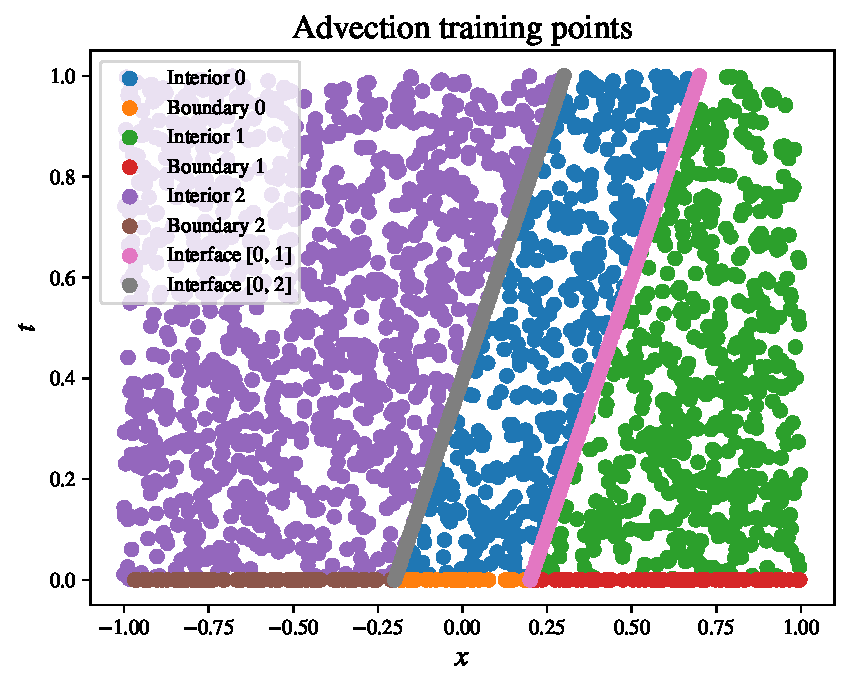
\includegraphics[width=0.9\linewidth]{Project1XPINNs/figures/advection/advection_train.pdf}
    \caption{Training points for the advection equation with the domain decomposed into three subdomains.}
    \label{fig:decomp_advection}
\end{figure}

In order to verify that our method is not simply learning the decomposition itself, we also verify that the wave is able to travel across the interfaces by setting $\alpha = -1$ while keeping the same decomposition.
Finally we compare our XPINN model with a single PINN training on the entire domain without any subdomains. 

Our network is composed of $6$ hidden layers, each with $20$ nodes, using $\tanh$ as our hidden activation function and no activation for the output layer. The learning rate is set to $10^{-4}$, with \textsc{Adam} as the optimizer.
We utilize $2000$ points for the interior, and $200$ evenly spread around the boundary and interfaces. 

\subsubsection{Results}
We run the models for 10 000 epochs each.
The resulting predictions are seen in \autoref{fig:advection_xpinn_pred}, closely fitting the true solution.
The absolute errors against the true solution can be seen in \autoref{fig:advection_xpinn_error}, where most of the error is found along the interfaces.
This is unsurprising, given the discontinuities along the boundaries.


\begin{figure}[h]
    \centering
    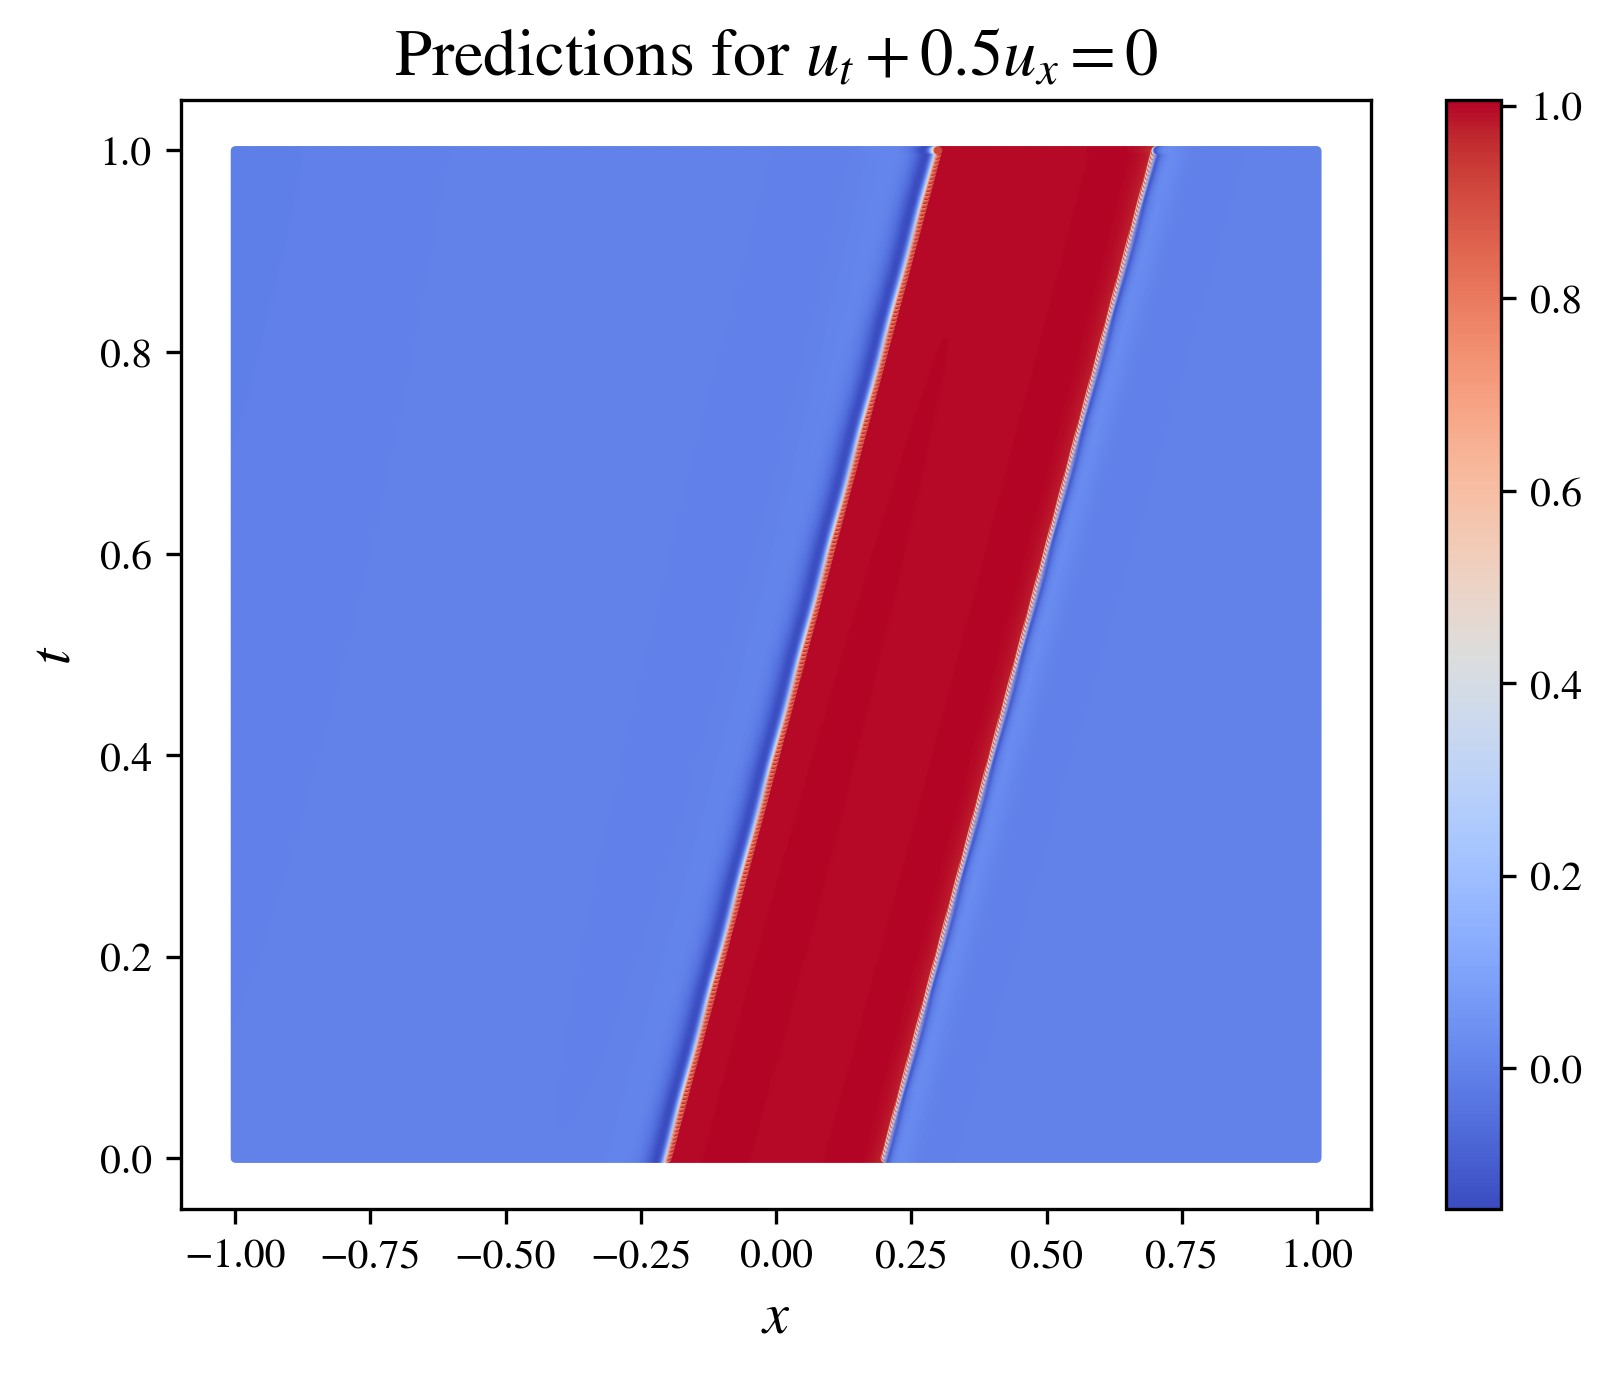
\includegraphics[width=0.8\linewidth]{Project1XPINNs/figures/advection/xpinn_predictions.png}
    \caption{XPINN Predictions for the advection equation.}\label{fig:advection_xpinn_pred}
\end{figure}

\begin{figure}[!h]
    \centering
    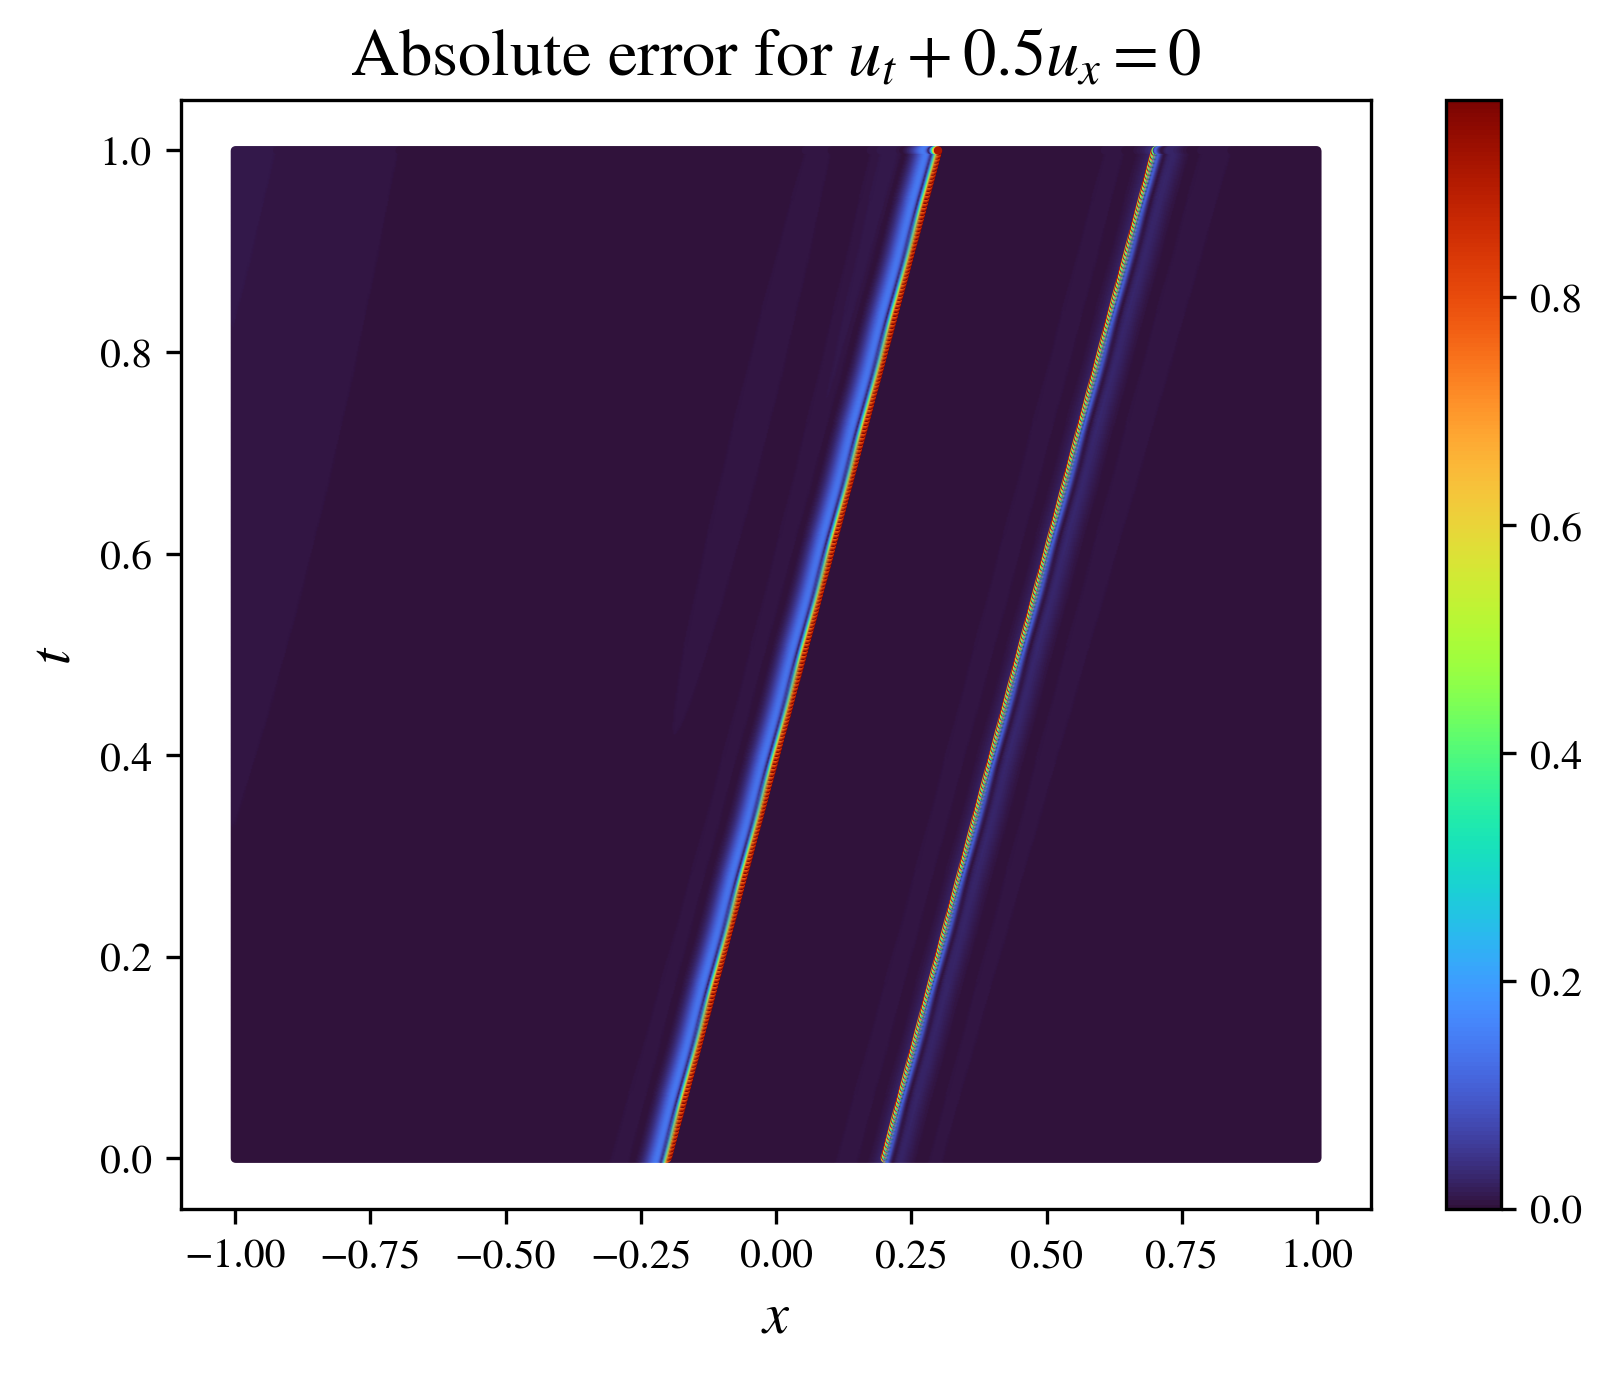
\includegraphics[width=0.8\linewidth]{Project1XPINNs/figures/advection/xpinn_error.png}
    \caption{Absolute error against the true solution, XPINN with $\alpha=0.5$.}\label{fig:advection_xpinn_error}
\end{figure}

The loss per epoch is shown in \autoref{fig:loss_per_advection}.
It is interesting to note how the different sub-PINNs adjust in accordance with each other, wherein the reduction in the loss of one sub-PINN often leads to an increase in the others, while the total loss is reduced.
Do note that the model seems to still be improving after 10 000 epochs, and that the learning rate needs further tuning.
We chose to not optimize this problem fully, as we were more interested in learning more about the behaviour of XPINNs, and seeing if our implementation had any merit.

\begin{figure}[h]
    \centering
    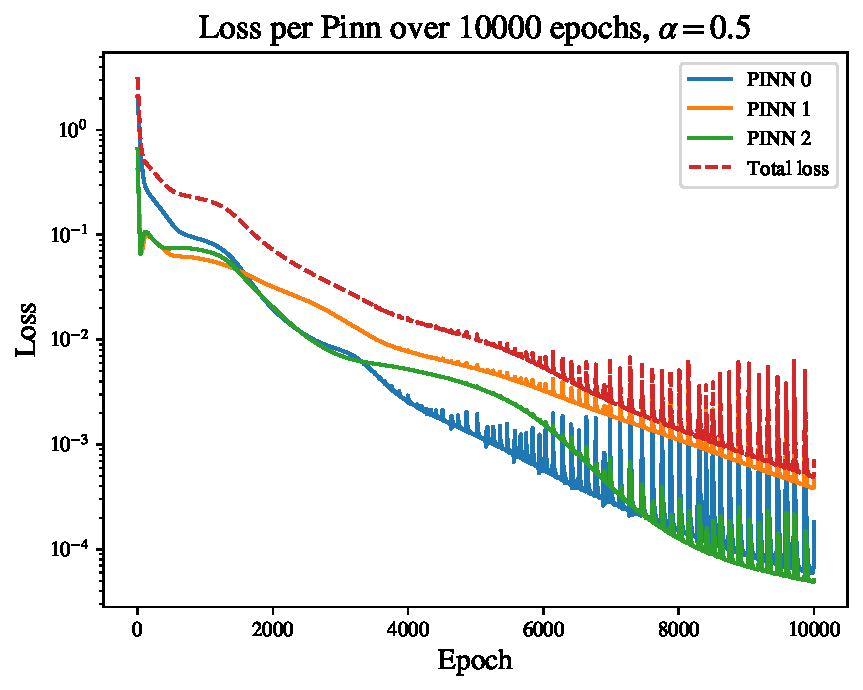
\includegraphics[width=0.8\linewidth]{Project1XPINNs/figures/advection/advection_losses.pdf}
    \caption{Loss per epoch for the advection equation with an XPINN, with $\alpha=0.5$.}
    \label{fig:loss_per_advection}
\end{figure}

Comparing against how a single PINN on the entire domain performs, we see better and more stable results from running the same number of epochs.
The predicted values are shown in \autoref{fig:single_ad_pred}, with the errors in \autoref{fig:single_ad_error}.
XPINNs then probably do not have a lot of merit for such a simple problem, especially given the simplicity of deriving the analytical solution.

\begin{figure}[h]
    \centering
    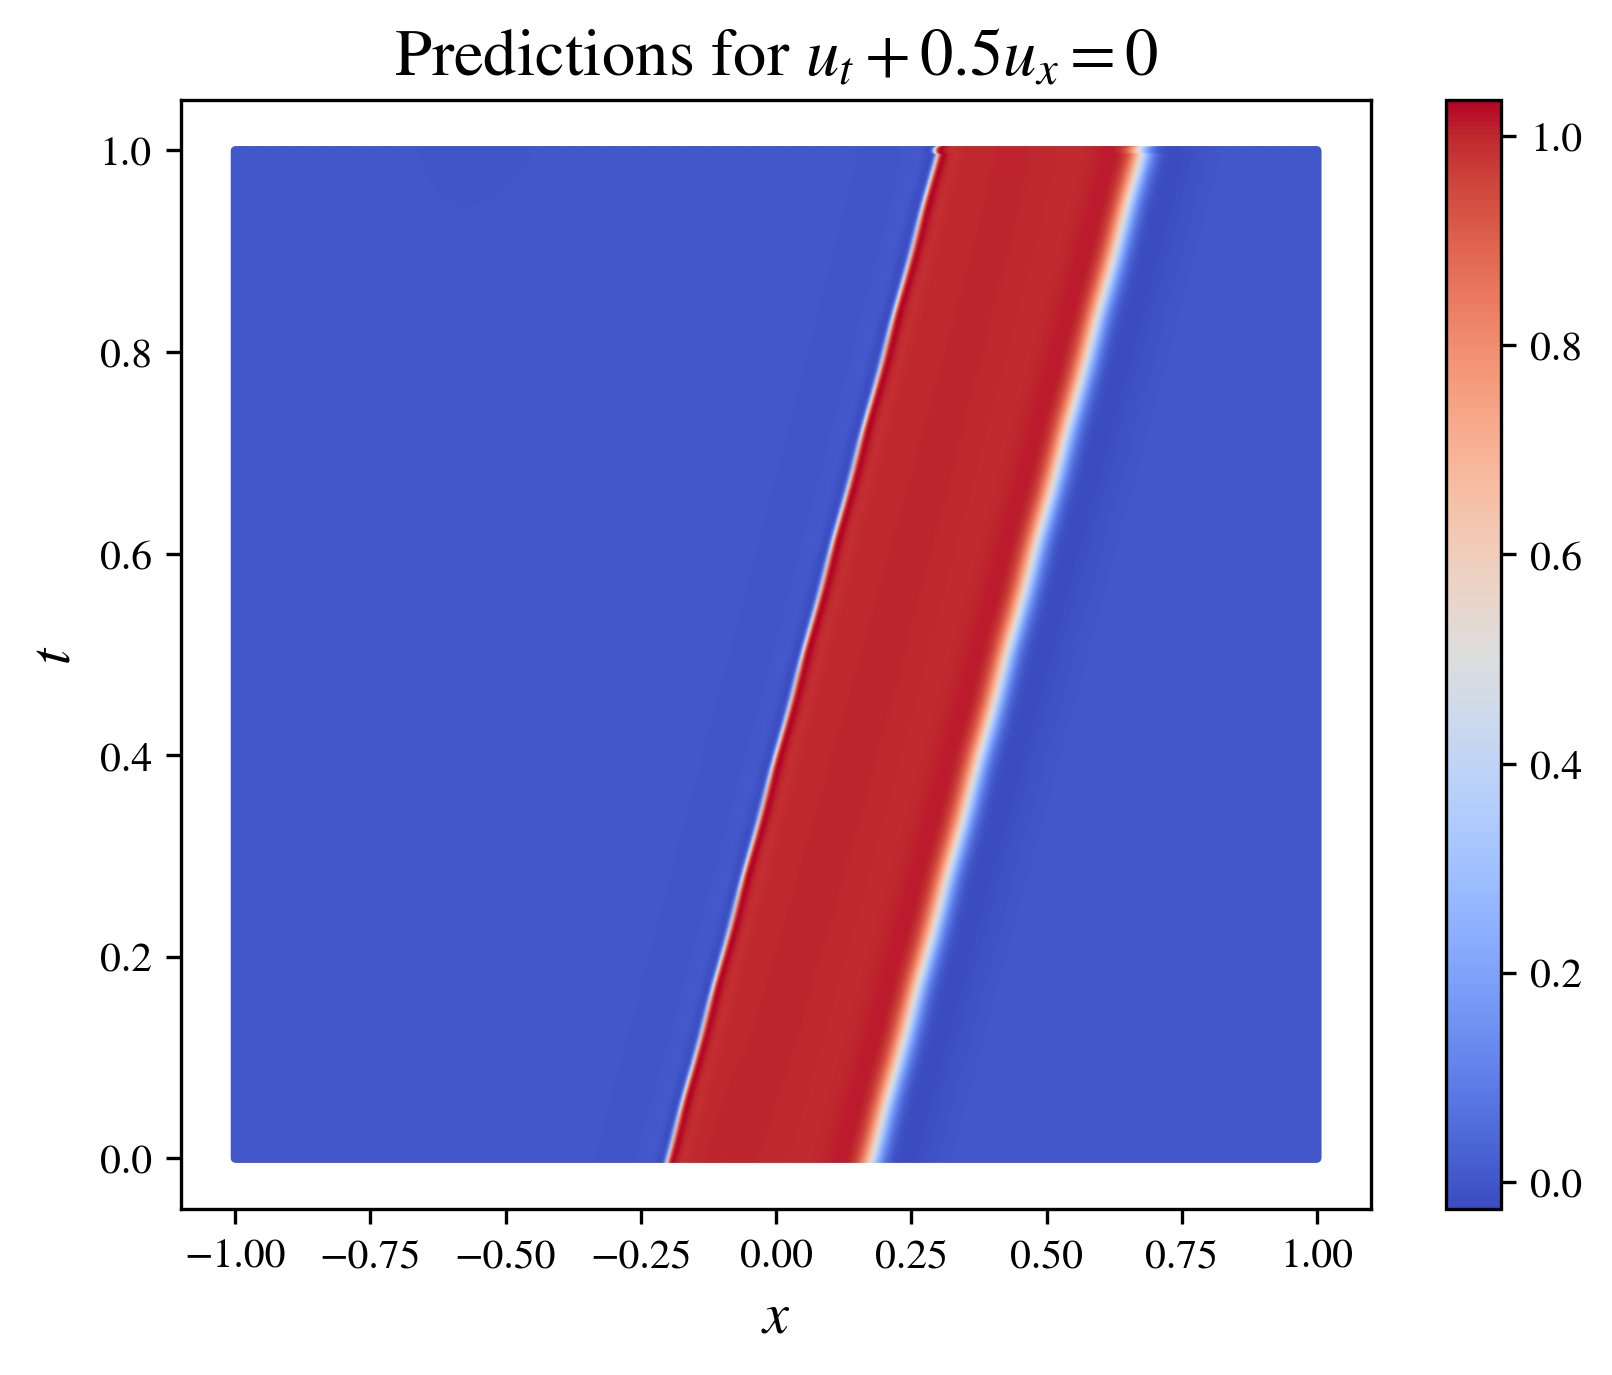
\includegraphics[width=0.8\linewidth]{Project1XPINNs/figures/advection/single_advection_predictions.png}
    \caption{Predicted values with a PINN.}
    \label{fig:single_ad_pred}
\end{figure}

\begin{figure}[h]
    \centering
    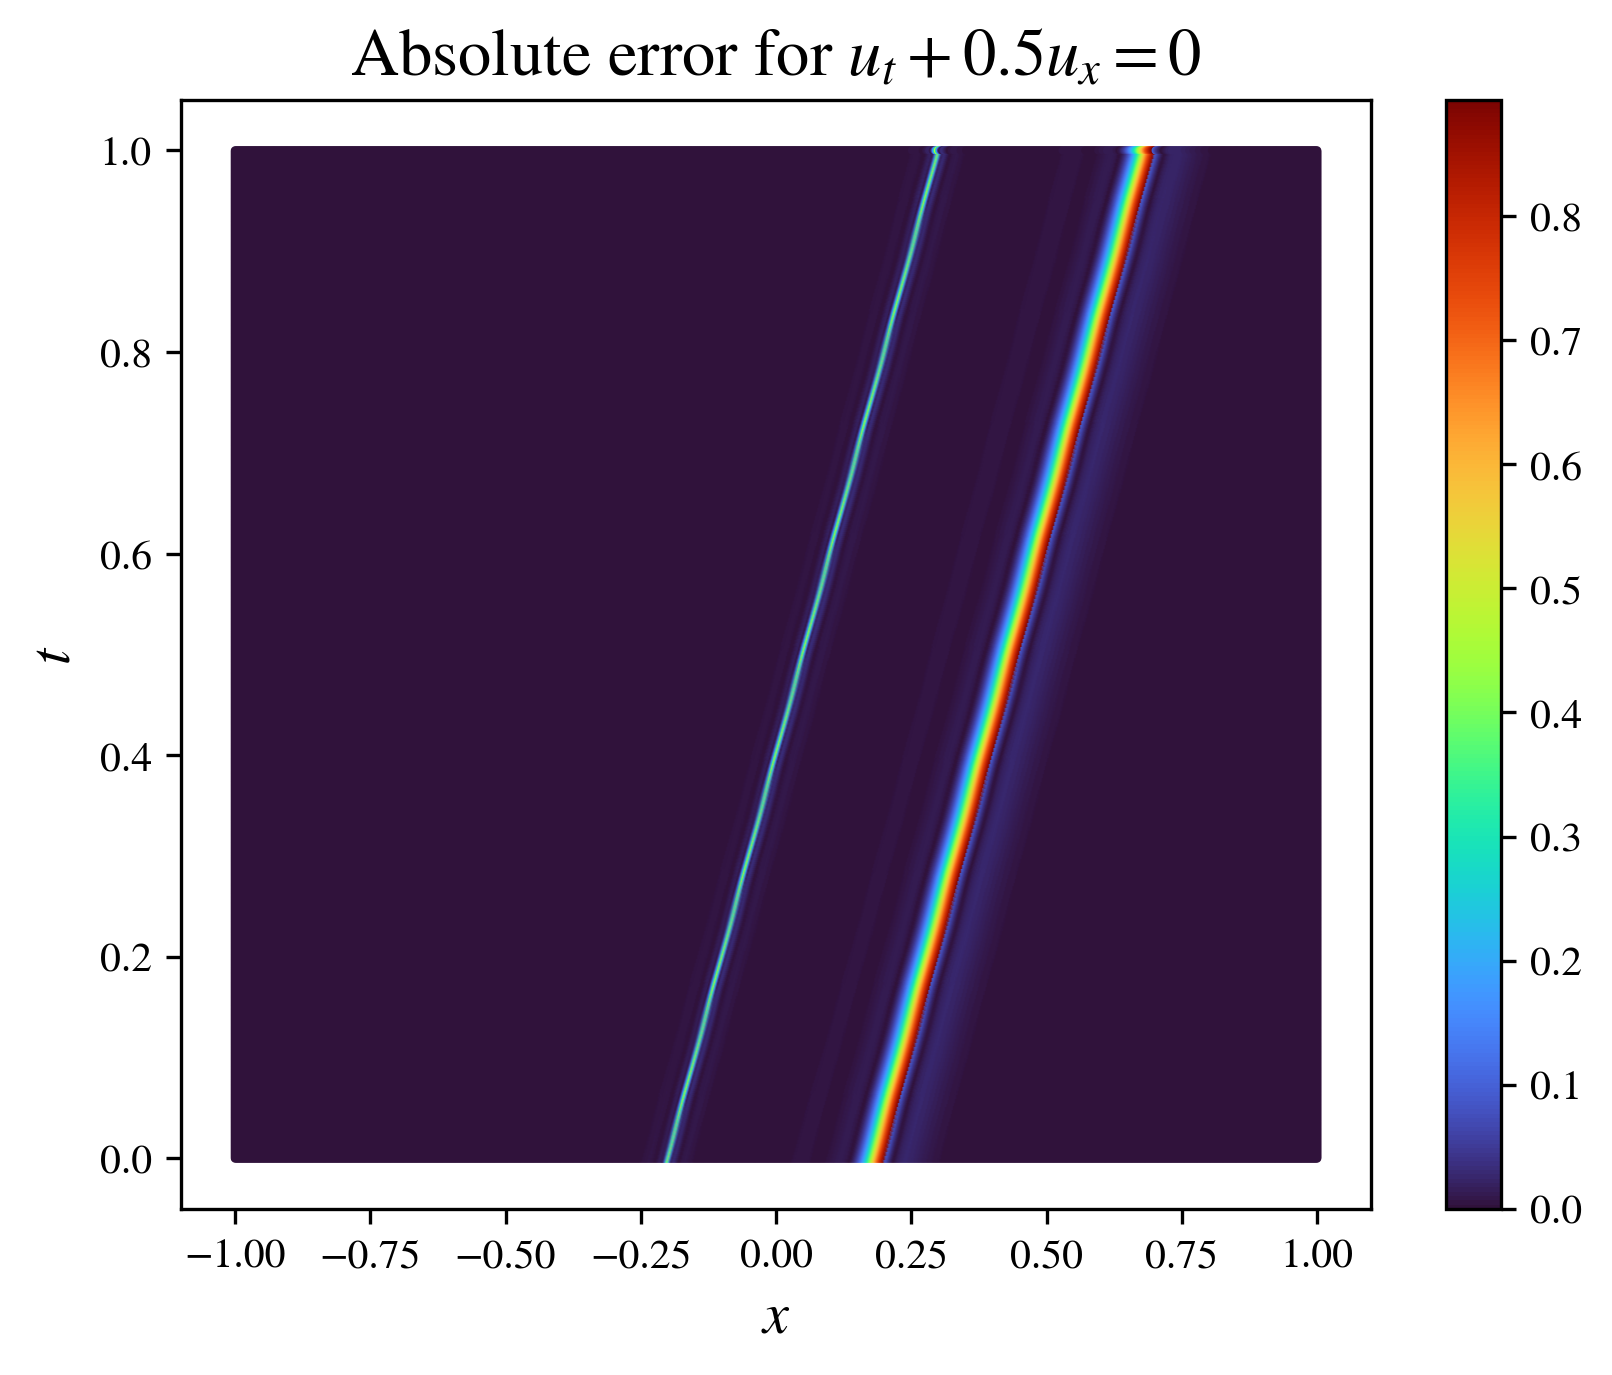
\includegraphics[width=0.8\linewidth]{Project1XPINNs/figures/advection/single_advection_error.png}
    \caption{Absolute errors with a PINN.}
    \label{fig:single_ad_error}
\end{figure}

We stress test our model by changing the equation in question by setting $\alpha=-1$, while keeping the same domain decomposition.
This is done in order to ensure that the XPINN is not simply learning the domain decomposition, but rather the behaviour we are expecting.
The wave is now able to traverse across the subdomain decomposition, as in \autoref{fig:alpha-1_pred}, however with worse errors in \autoref{fig:alpha-1_error} than we saw previously.
This is a promising result before moving on to more difficult problems.

\begin{figure}[h!]
    \centering
    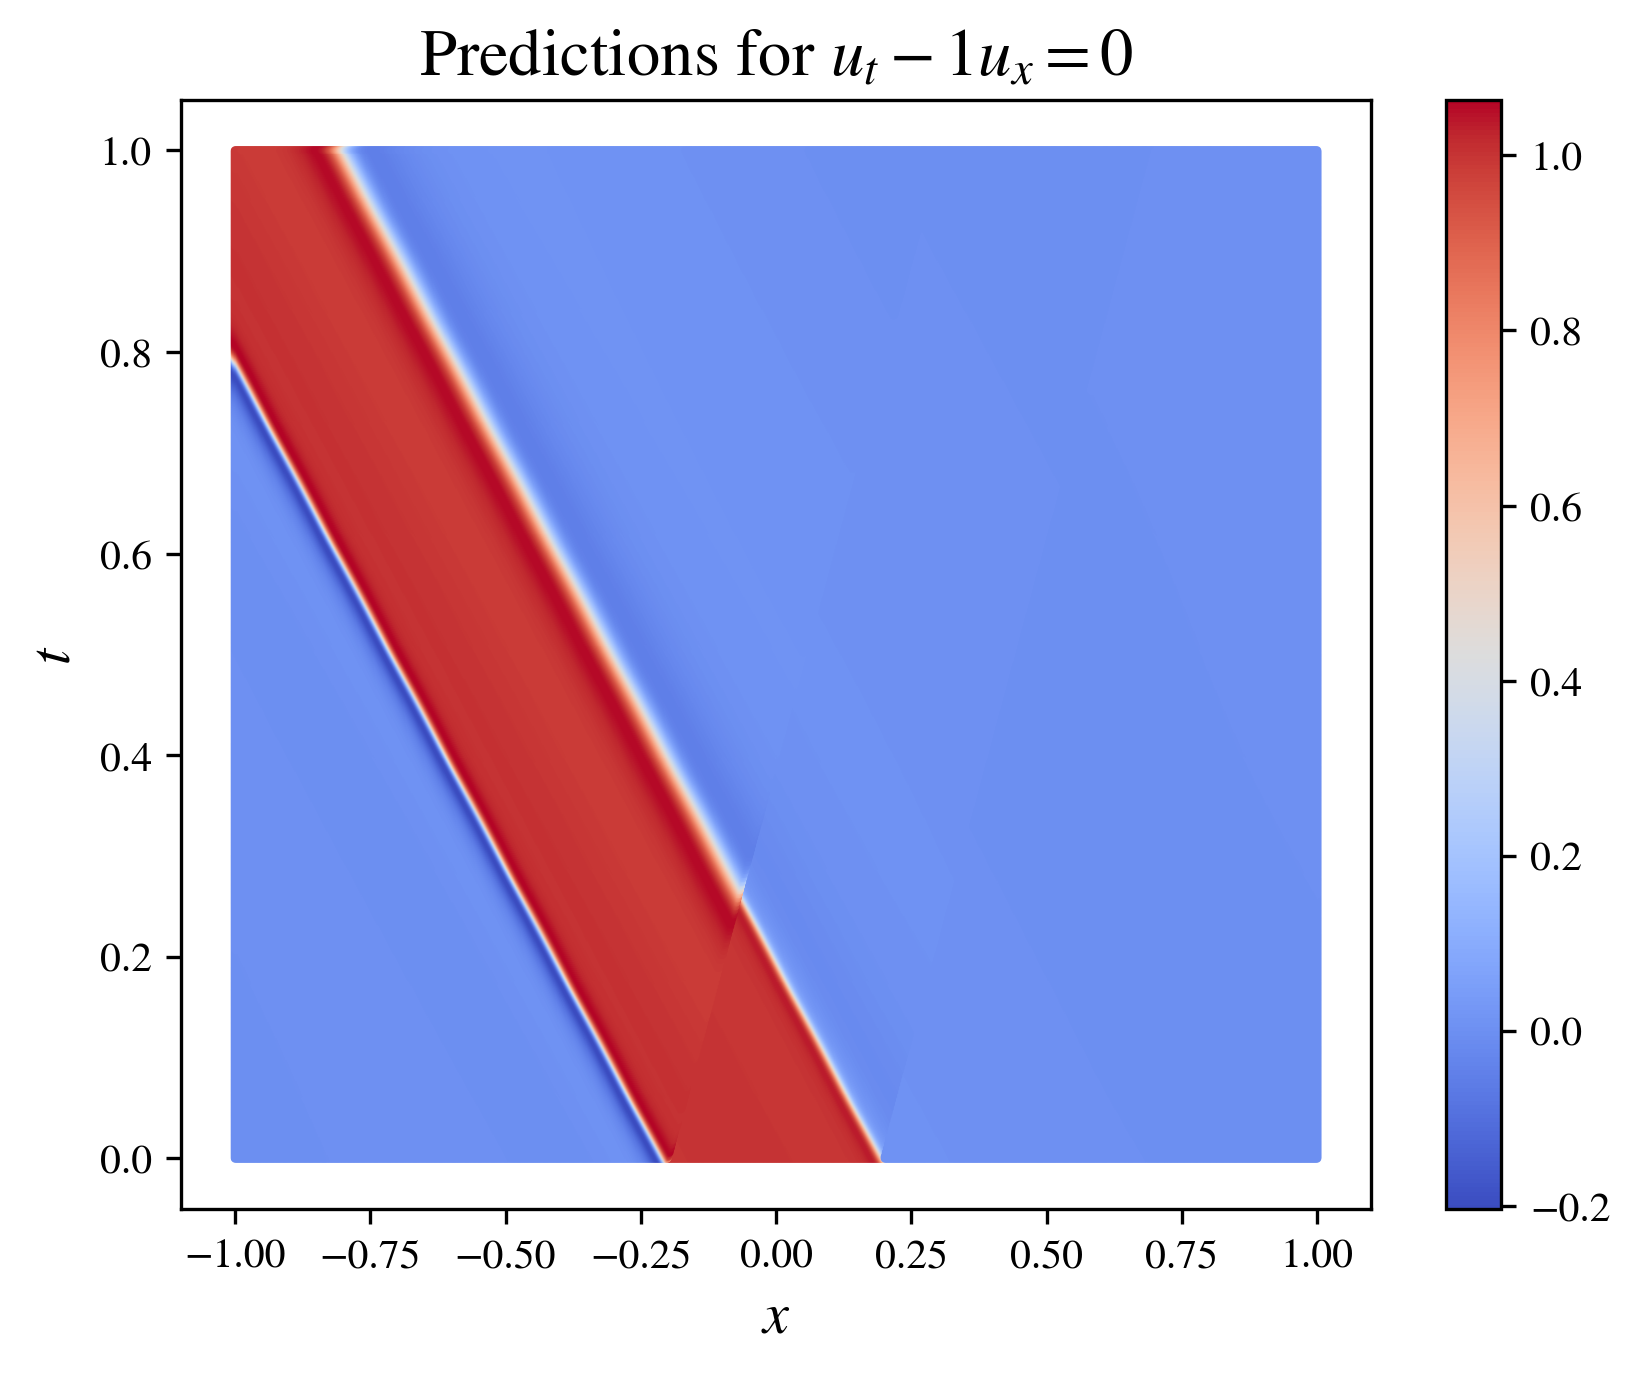
\includegraphics[width=0.8\linewidth]{Project1XPINNs/figures/advection/xpinn_stress_predictions.png}
    \caption{XPINN predictions with $\alpha=-1$.}
    \label{fig:alpha-1_pred}
\end{figure}
\begin{figure}[h!]
    \centering
    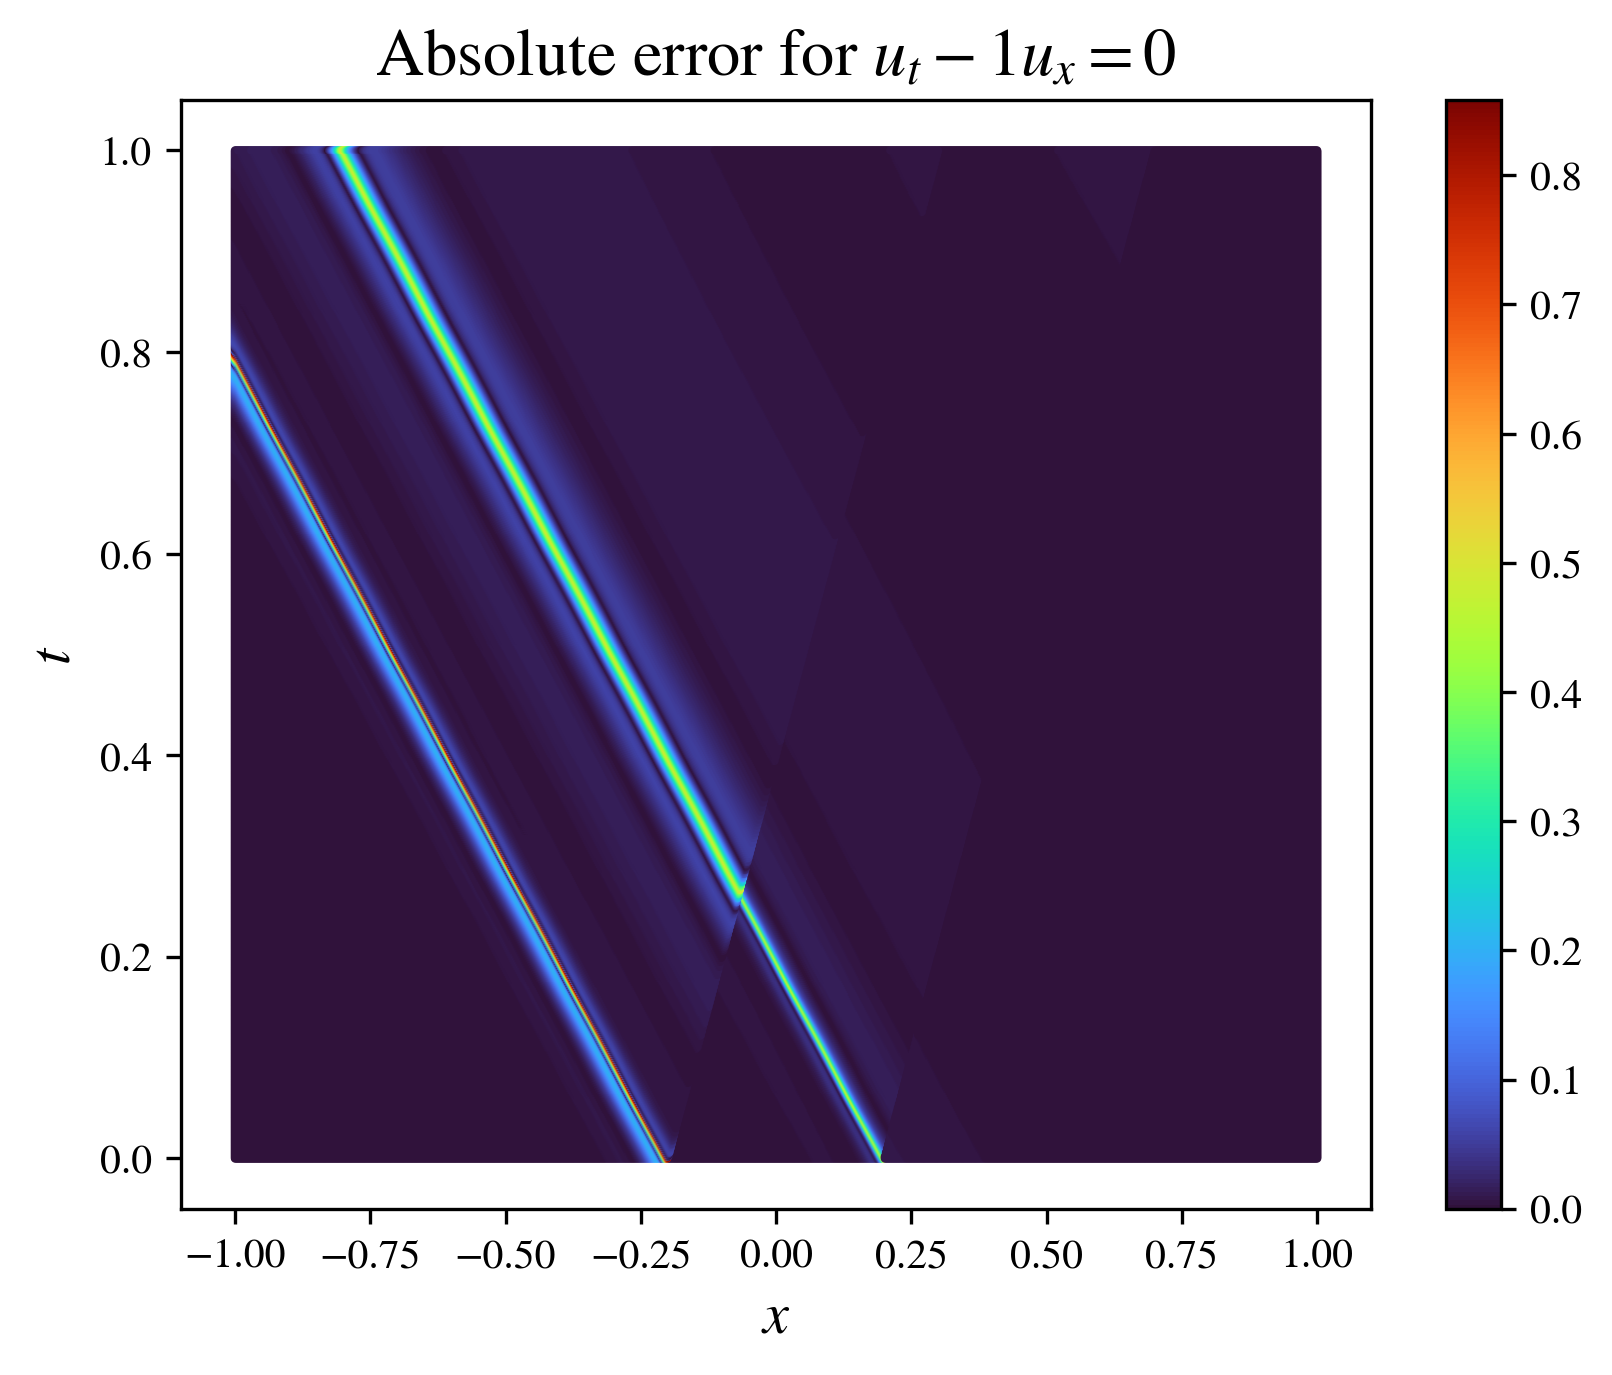
\includegraphics[width=0.8\linewidth]{Project1XPINNs/figures/advection/xpinn_stress_error.png}
    \caption{Absolute error with $\alpha=-1$.}
    \label{fig:alpha-1_error}
\end{figure}

% \vfill\null

\subsection{Poisson Equation}
\subsubsection{Problem Formulation}
In this subsection, we consider a two-dimensional inhomogeneous Poisson equation with residual.
The problem is a second order linear PDE, and is defined as
\begin{align}\label{eq:poisson}
\begin{cases}
    u_{xx}+u_{yy} = f &\text{on } \Omega \\
    u(x,y) = 0 &\text{on } \partial\Omega,
\end{cases}
\end{align}
where $\Omega = [0,1] \times [0,1]$.
For the Poisson equation, we consider both a continuous and a discontinuous residual.

\paragraph{Continuous Residual:}
The first residual is given by
\begin{equation}\label{eq:continuous_poisson}
    f_{\text{cont}}(x,y)= -2\pi^2\sin(\pi x) \sin(\pi y),
\end{equation}
which yields the known analytical solution
\begin{equation*}
    u_{\text{true}}(x,y)=\sin(\pi x) \sin(\pi y),
\end{equation*}
which is displayed in \autoref{fig:exact_smooth}.

\begin{figure}[h]
    \centering
    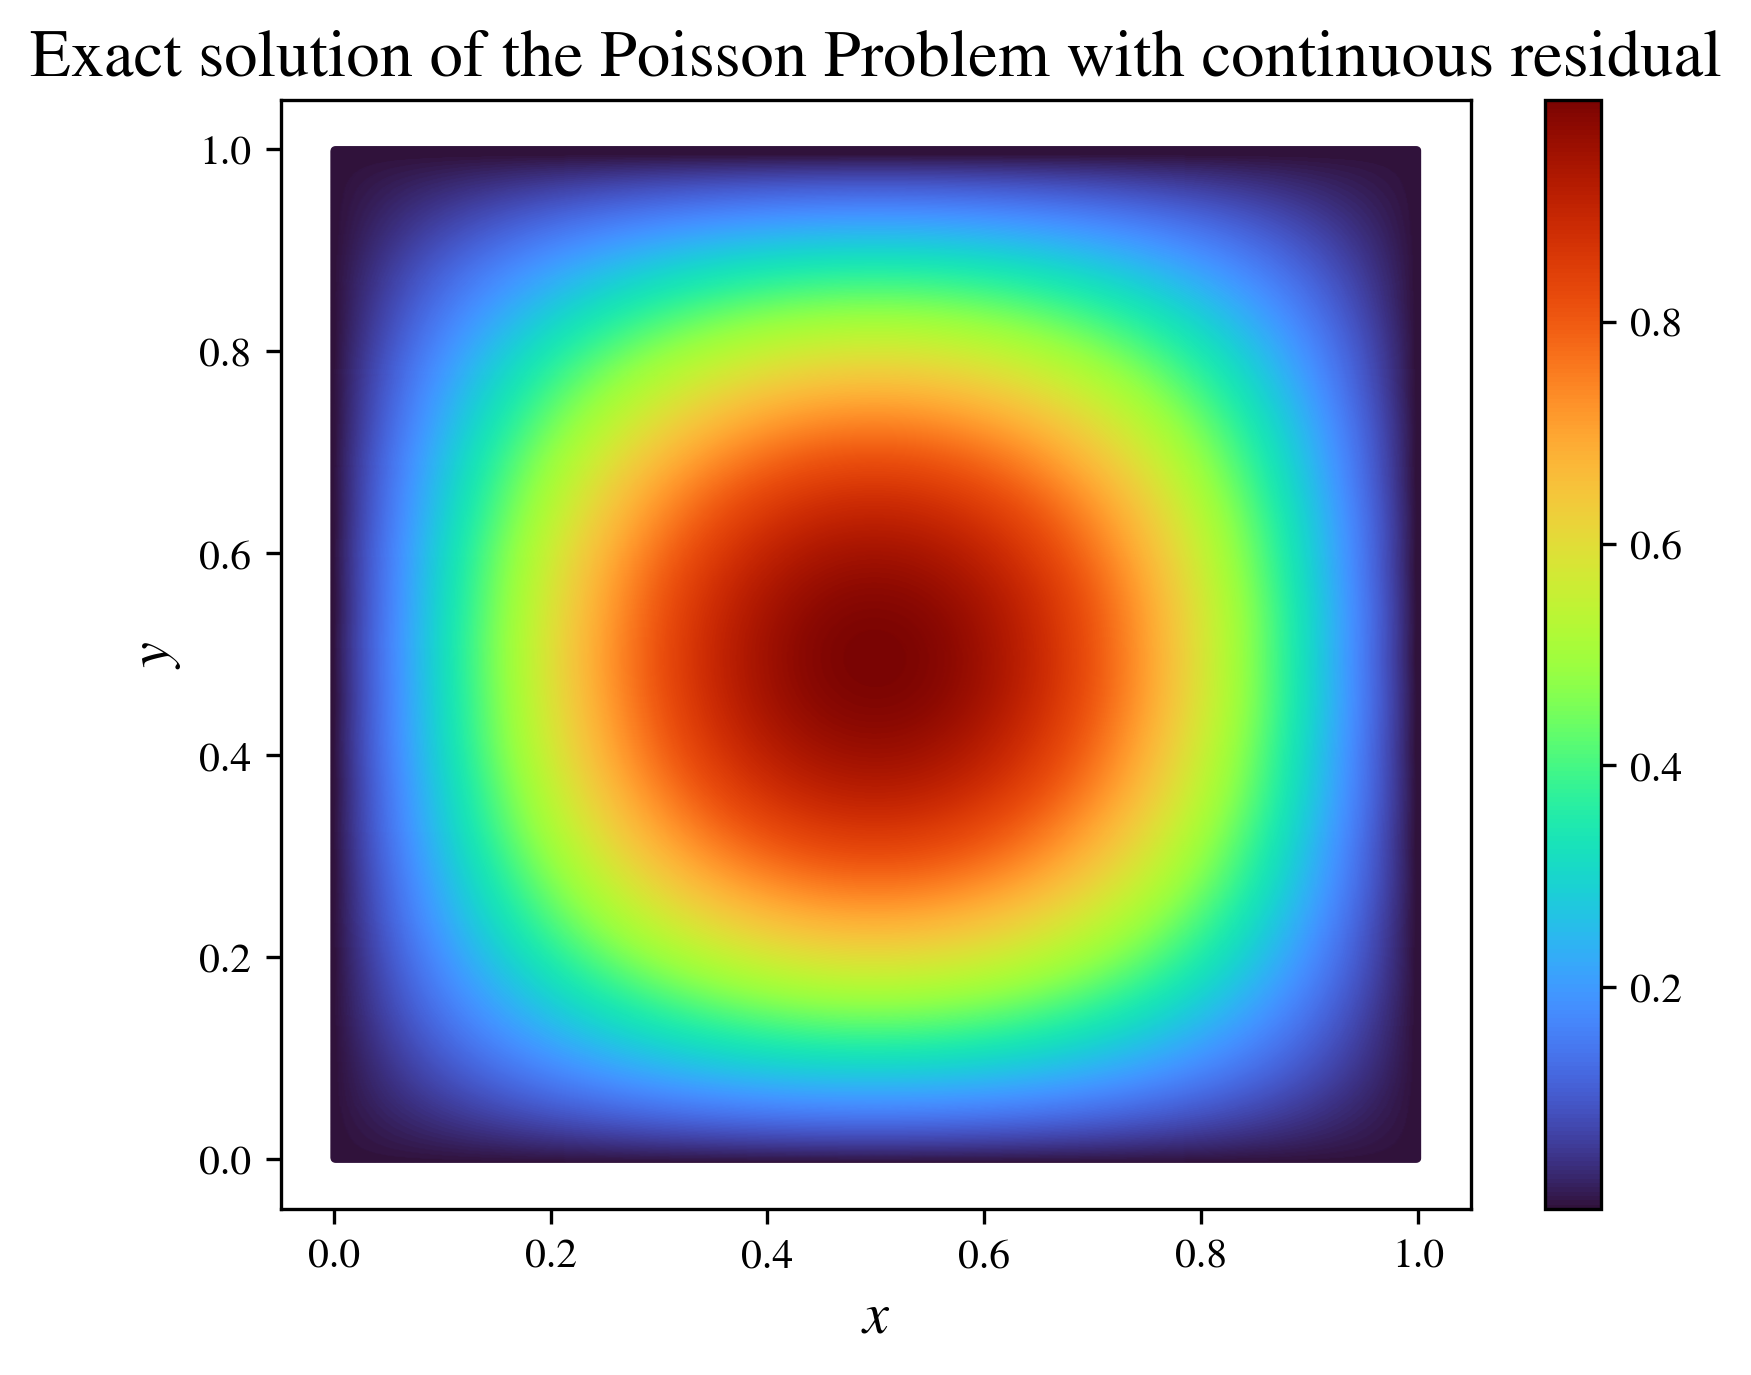
\includegraphics[width=0.8\linewidth]{Project1XPINNs/figures/Poisson/smooth_Poisson_true.png}
    \caption{The exact analytical solution to the Poisson equation with continuous residual.}
    \label{fig:exact_smooth}
\end{figure}

Our experimental setup follows that of \textcite{müller2023achieving}.
We consider the problem for both a single PINN and for an XPINN decomposition shown in \autoref{fig:decomp_poisson}.
For the PINN, we train using 900 interior points and 120 boundary points distributed uniformly.
For the XPINN, we also add 80 uniformly distributed interface points. Thus, the total amount of training points used for the XPINN exceeds that for the PINN.
We apply unitary weights to the different losses.
All PINNs have the same architecture of a 3-layered neural network with 64 hidden units, and we use the $\tanh$ activation function. 
Both solvers are trained using the \textsc{Adam} optimizer with an exponentially decreasing learning rate.
The initial learning rate is $10^{-3}$.
After $1.5\times 10^4$ steps, we decrease the learning rate by a factor of $10^{-1}$ every $10^4$ steps until a minimum learning rate of $10^{-7}$.
We train both cases for $2\times 10^5$ iterations. For our testing, we consider a uniform grid with 1 000 000 points. 

\begin{figure}[h]
    \centering
    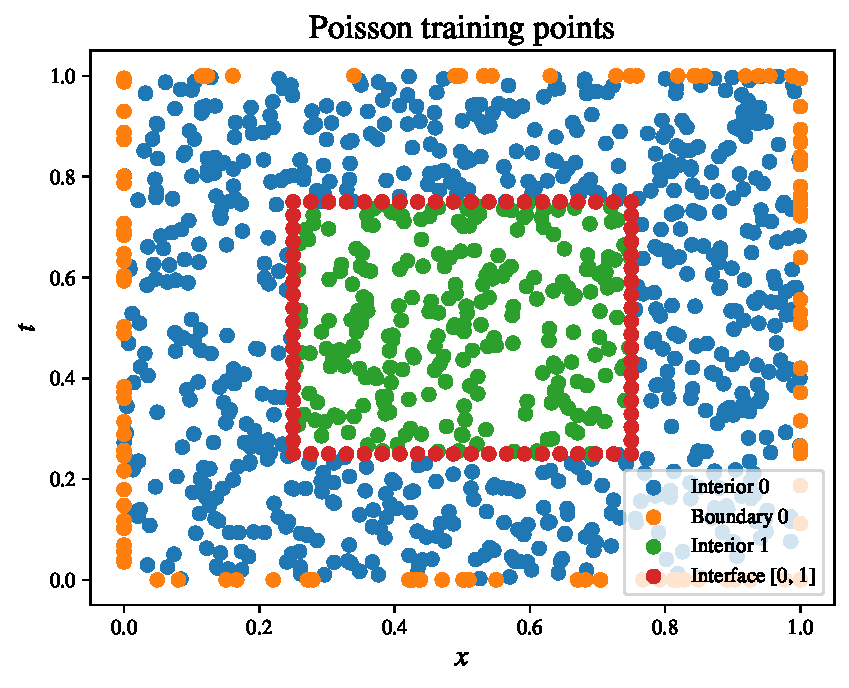
\includegraphics[width=0.9\linewidth]{Project1XPINNs/figures/Poisson/poisson_train_points.pdf.pdf}
    \caption{Training points with the XPINN decomposition for the Poisson equation. The PINN is given the same points, without the interface points.}
    \label{fig:decomp_poisson}
\end{figure}

\vspace{-1cm}
\paragraph{Discontinuous Residual:}
The second residual is due \textcite{XPINN_generalize}, where they compare the generalizeability of PINNs and XPINNs.
The residual is given as a discontinuous form
\begin{equation*}\label{eq:discontinuous_poisson}
    f_{disc}(x,y)=
    \begin{cases}
        1 &\text{if} \, (x,y)\in [0.25,0.75]\times[0.25,0.75], \\
        0 &\text{else}.
    \end{cases}
\end{equation*}

The reference solution is computed numerically using the \verb|poissonpy| package \cite{poissonpy} on a uniform test mesh with 1 000 000 points, displayed in \autoref{fig:exact_discontinuous}.
We apply a 9 layer neural network with 20 hidden units, using the $\tanh$ activation function.
Again, we apply 900 internal, 120 boundary and 80 interface points for training the XPINN model, as in \autoref{fig:decomp_poisson}.
Additionally, we apply 20 weights to the boundary conditions for the PINN, and 20 for boundary and interface conditions for our XPINN. 
\textsc{Adam} is again used, and the solvers are run for $2\times 10^5$ iterations. The exponential decay rate is the same as in the continuous experiment, although the minimum learning rate is set as $10^{-5}$.

Note that the paper by \textcite{XPINN_generalize} uses the LBFGS optimizer, however this method is not implemented in our chosen optimization library \verb|optax|.
LBFGS is available in \verb|JAXopt| \cite{jaxopt_implicit_diff}.
However, \verb|JAXopt| is currently being merged into \verb|optax|.
Adapting our implementation to be compatible with \verb|JAXopt| falls outside the scope of this project.

\begin{figure}[!h]
    \centering
    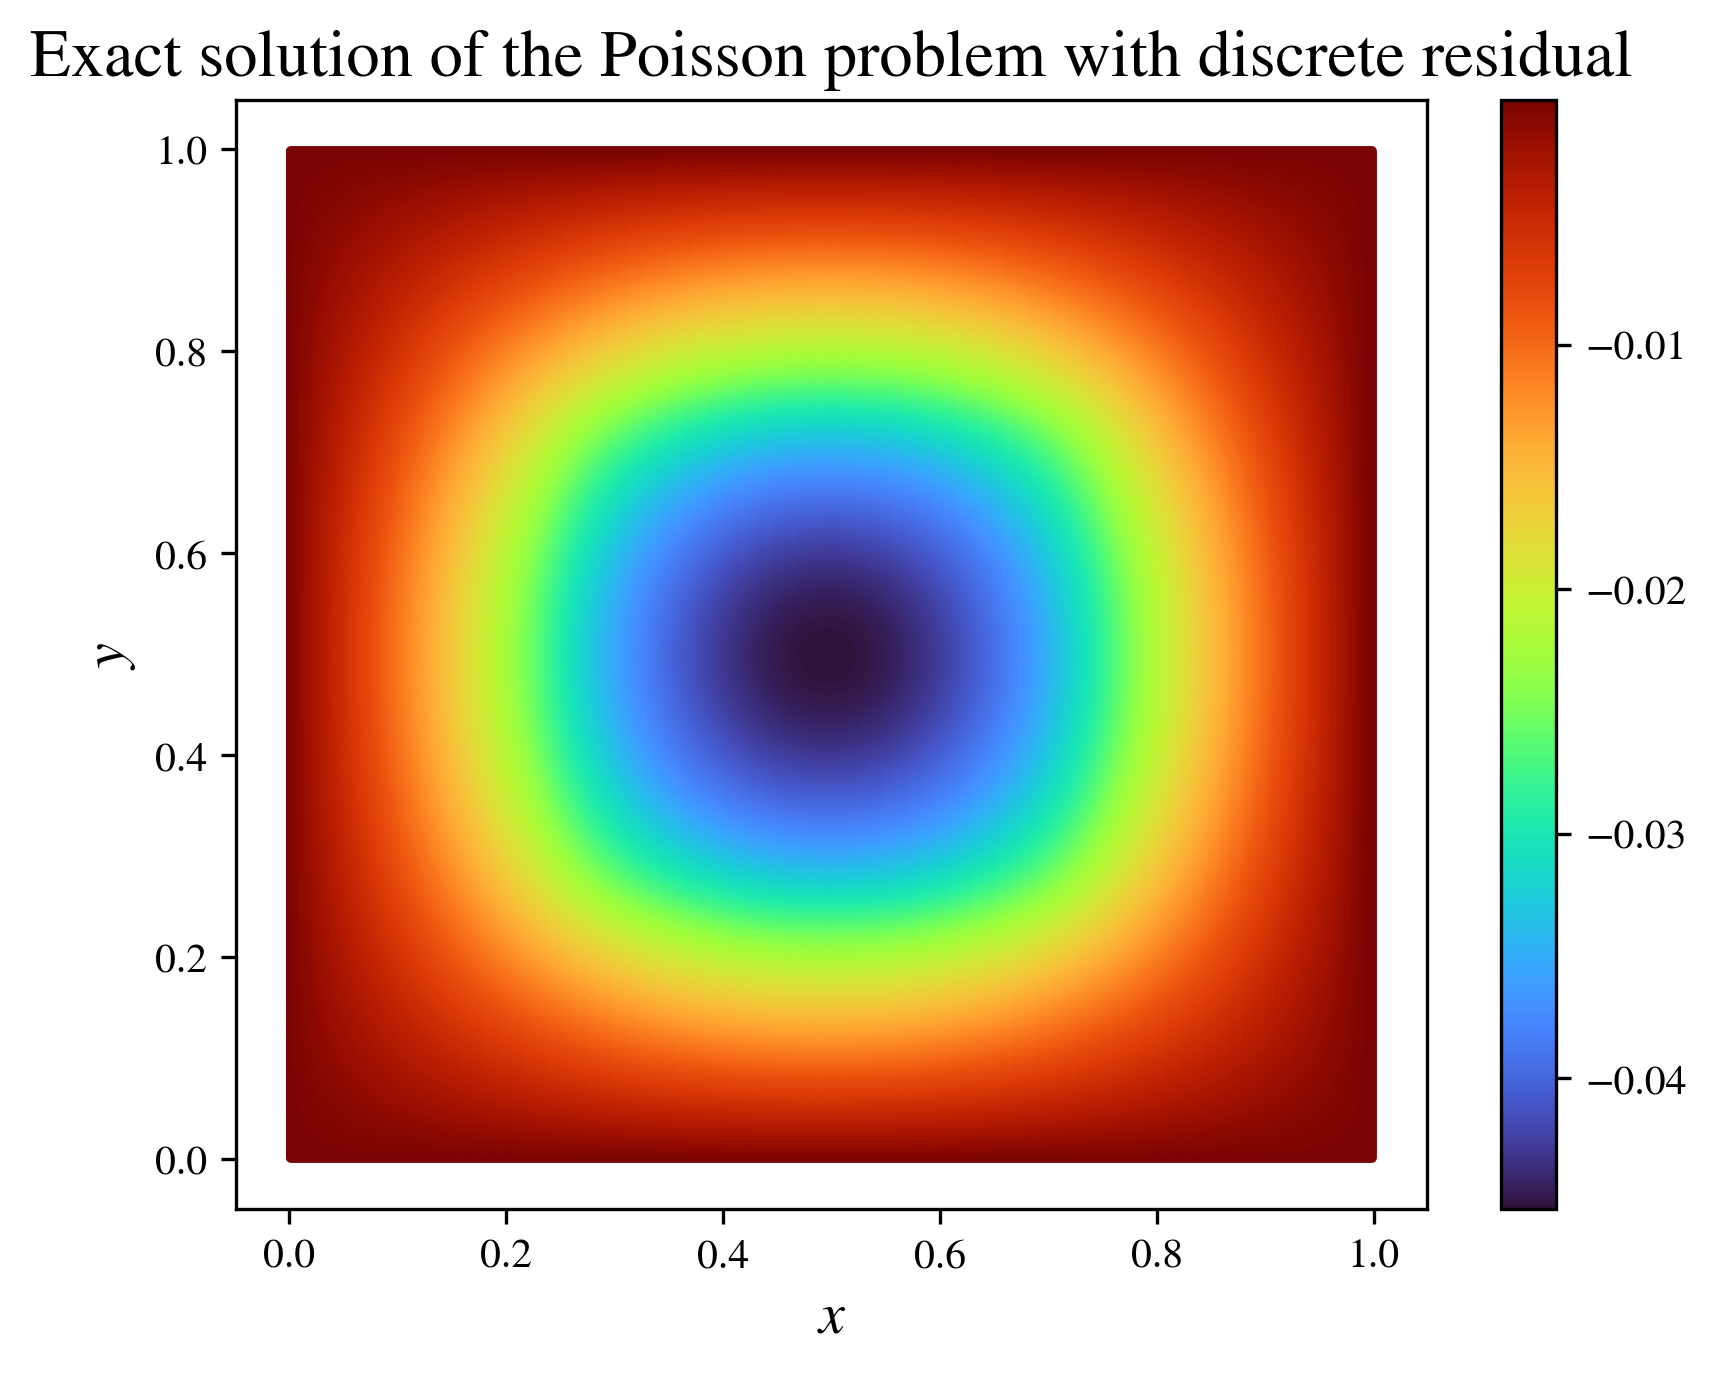
\includegraphics[width = 0.8\linewidth]{Project1XPINNs/figures/Poisson/discrete_Poisson_solution.png}
    \caption{Numerically computed reference solution to the Poisson equation with discontinuous residual.}
    \label{fig:exact_discontinuous}
\end{figure}
% \vfill\null

\subsubsection{Results}
\paragraph{Continuous Residual:}
\autoref{table:cont_poisson} shows the minimum, median, and maximum relative $L^2$ errors of the single PINN and XPINN solvers for the continuous residual Poisson equation using the \textsc{Adam} optimizer, across ten iterations.
Note that the training mesh was re-generated between each iteration.

% \vfill\null

\autoref{fig:rel_l2_smooth_poisson} displays the $L^2$ error evolution against the iterations.
From the figure, we see that the $L^2$ error seems to stabilize.
Although of similar orders of magnitude, we see that the PINN model frequently outperforms our XPINN discretization.
This is as expected by the argument of \textcite{XPINN_generalize}, as the domain decomposition does not reduce the target function complexity in the subdomains, whereas each subdomain trains on fewer points than the PINN. 

\begin{table}[h]
\caption{Median, minimum and maximum of the relative $L^2$-errors for the Poisson equation with continuous residual achieved by the PINN and XPINN.}
\centering
\begin{tabular}{r|c|c|c}\toprule
     & Median & Minimum & Maximum \\
    \colrule
    PINN & $1.37\cdot 10^{-3}$ &  $8.4 \cdot 10^{-4}$ & $2.16 \cdot 10^{-3}$ \\
    XPINN & $2.82\cdot 10^{-3} $ &  $1.23 \cdot 10^{-3}$ & $5.42 \cdot 10^{-3}$ \\
    \botrule
\end{tabular}
\label{table:cont_poisson}
\vspace{-0.5cm}
\end{table}
\begin{figure}[h!]
    \centering
    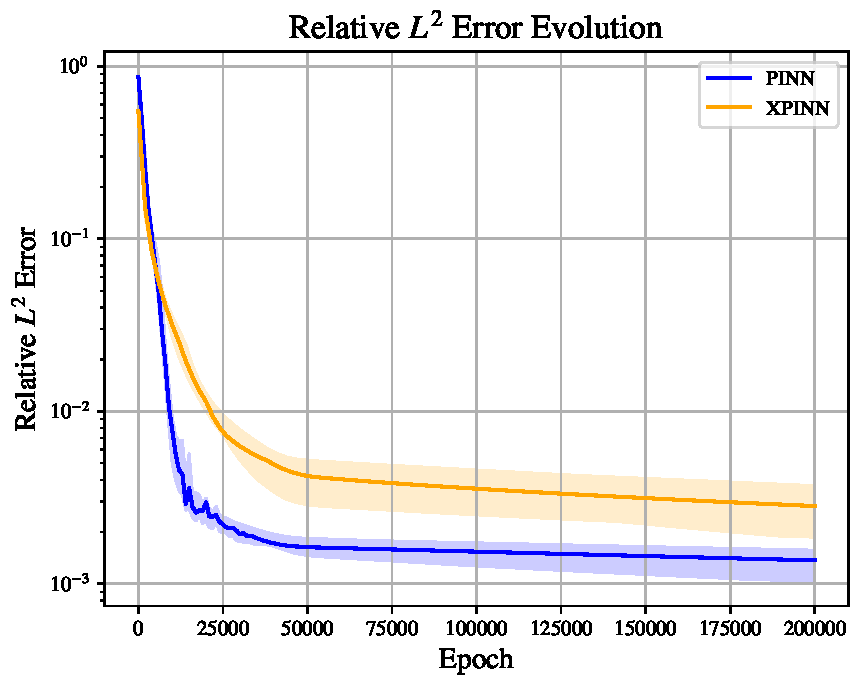
\includegraphics[width = 0.8\linewidth]{Project1XPINNs/figures/Poisson/smooth_l2_error_evolution.pdf}
    \caption{Relative $L^2$ error with median and interquartile range highlighted, for continuous residual.}
    \label{fig:rel_l2_smooth_poisson}
\end{figure}

The PINN and XPINN predictions are shown in \autoref{fig:pinn_smooth_pred} and \autoref{fig:xpinn_smooth_pred}, and although they are hard to distinguish visually, the errors displayed in \autoref{fig:pinn_smooth_error} and \autoref{fig:xpinn_smooth_error} tell a different story.
Note that the error figures are created with the same colorbar, in order to be comparable.
We note that the significant sources of error for the PINN appear to be surrounding the boundaries.
The XPINN solution also shows boundary error, but the interface error seems to dominate.
Optimizing for the different weighting hyper-parameters might lower the interface error, potentially at the cost of increased boundary error.

\begin{figure}[h]
    \centering
    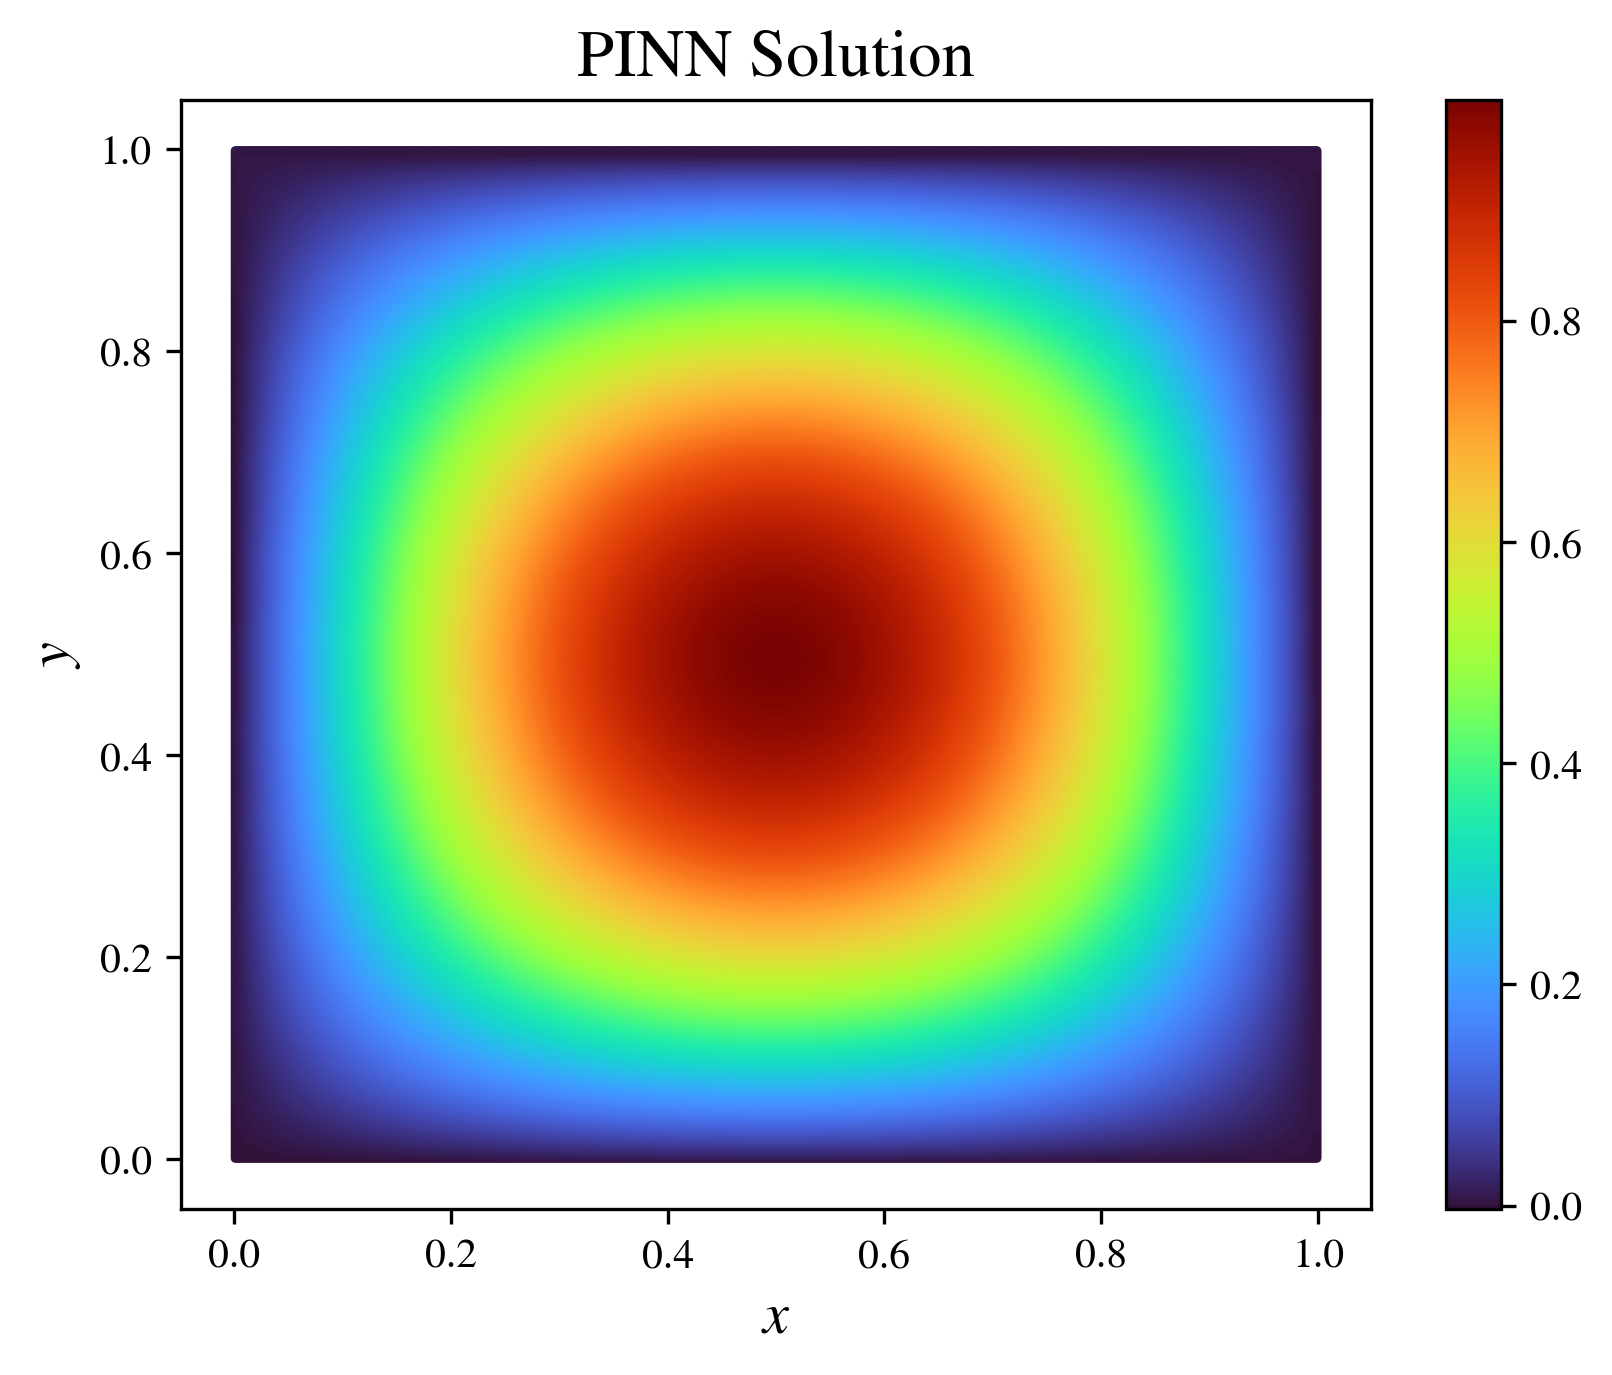
\includegraphics[width=\linewidth]{Project1XPINNs/figures/Poisson/smooth_single_Poisson_solution.png}
    \caption{PINN prediction with continuous residual.}
    \label{fig:pinn_smooth_pred}
\end{figure}
% \vspace{-1}

\begin{figure}[h]
    \centering
    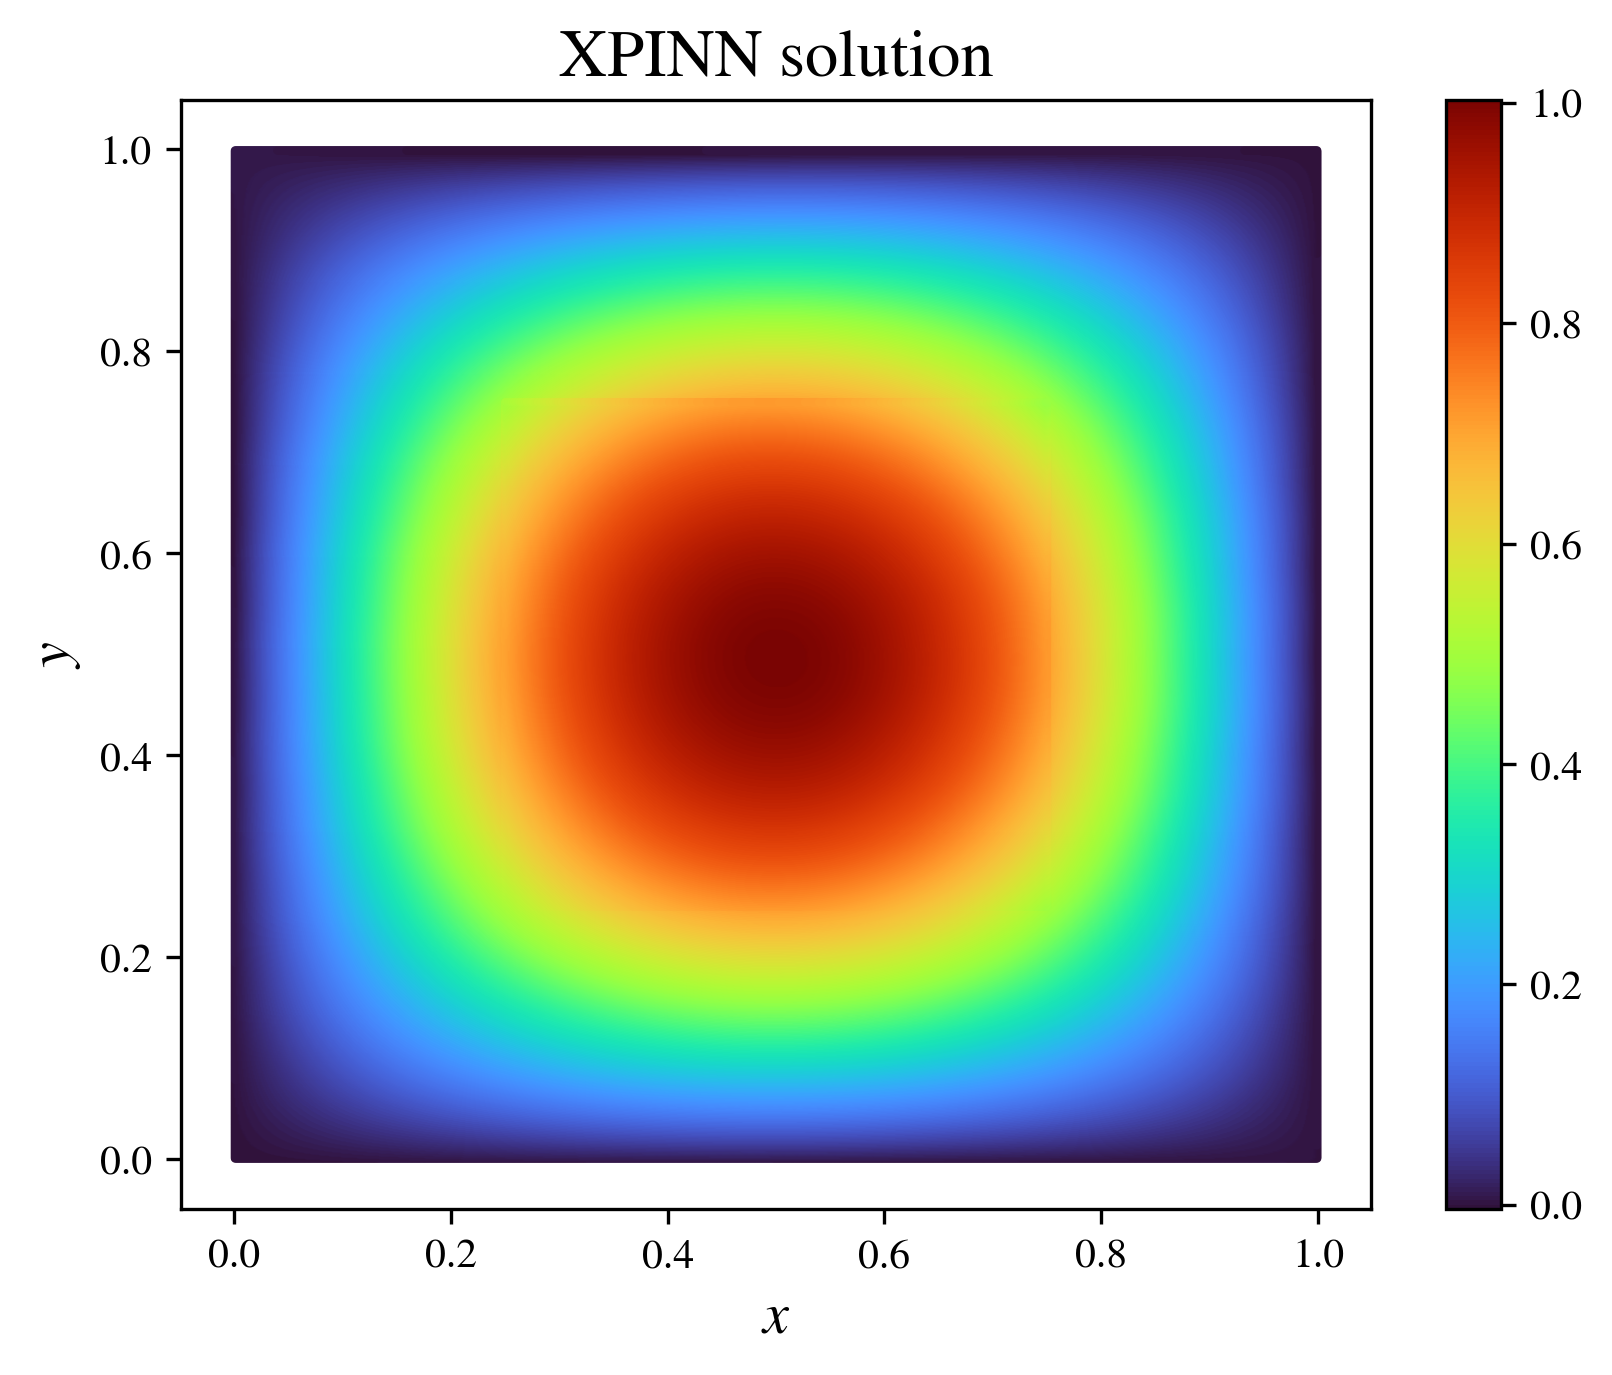
\includegraphics[width=\linewidth]{Project1XPINNs/figures/Poisson/smooth_xpinn_Poisson_solution.png}
    \caption{XPINN prediction with continuous residual.}
    \label{fig:xpinn_smooth_pred}
\end{figure}

% \vfill\null

\begin{figure}[h]
    \centering
    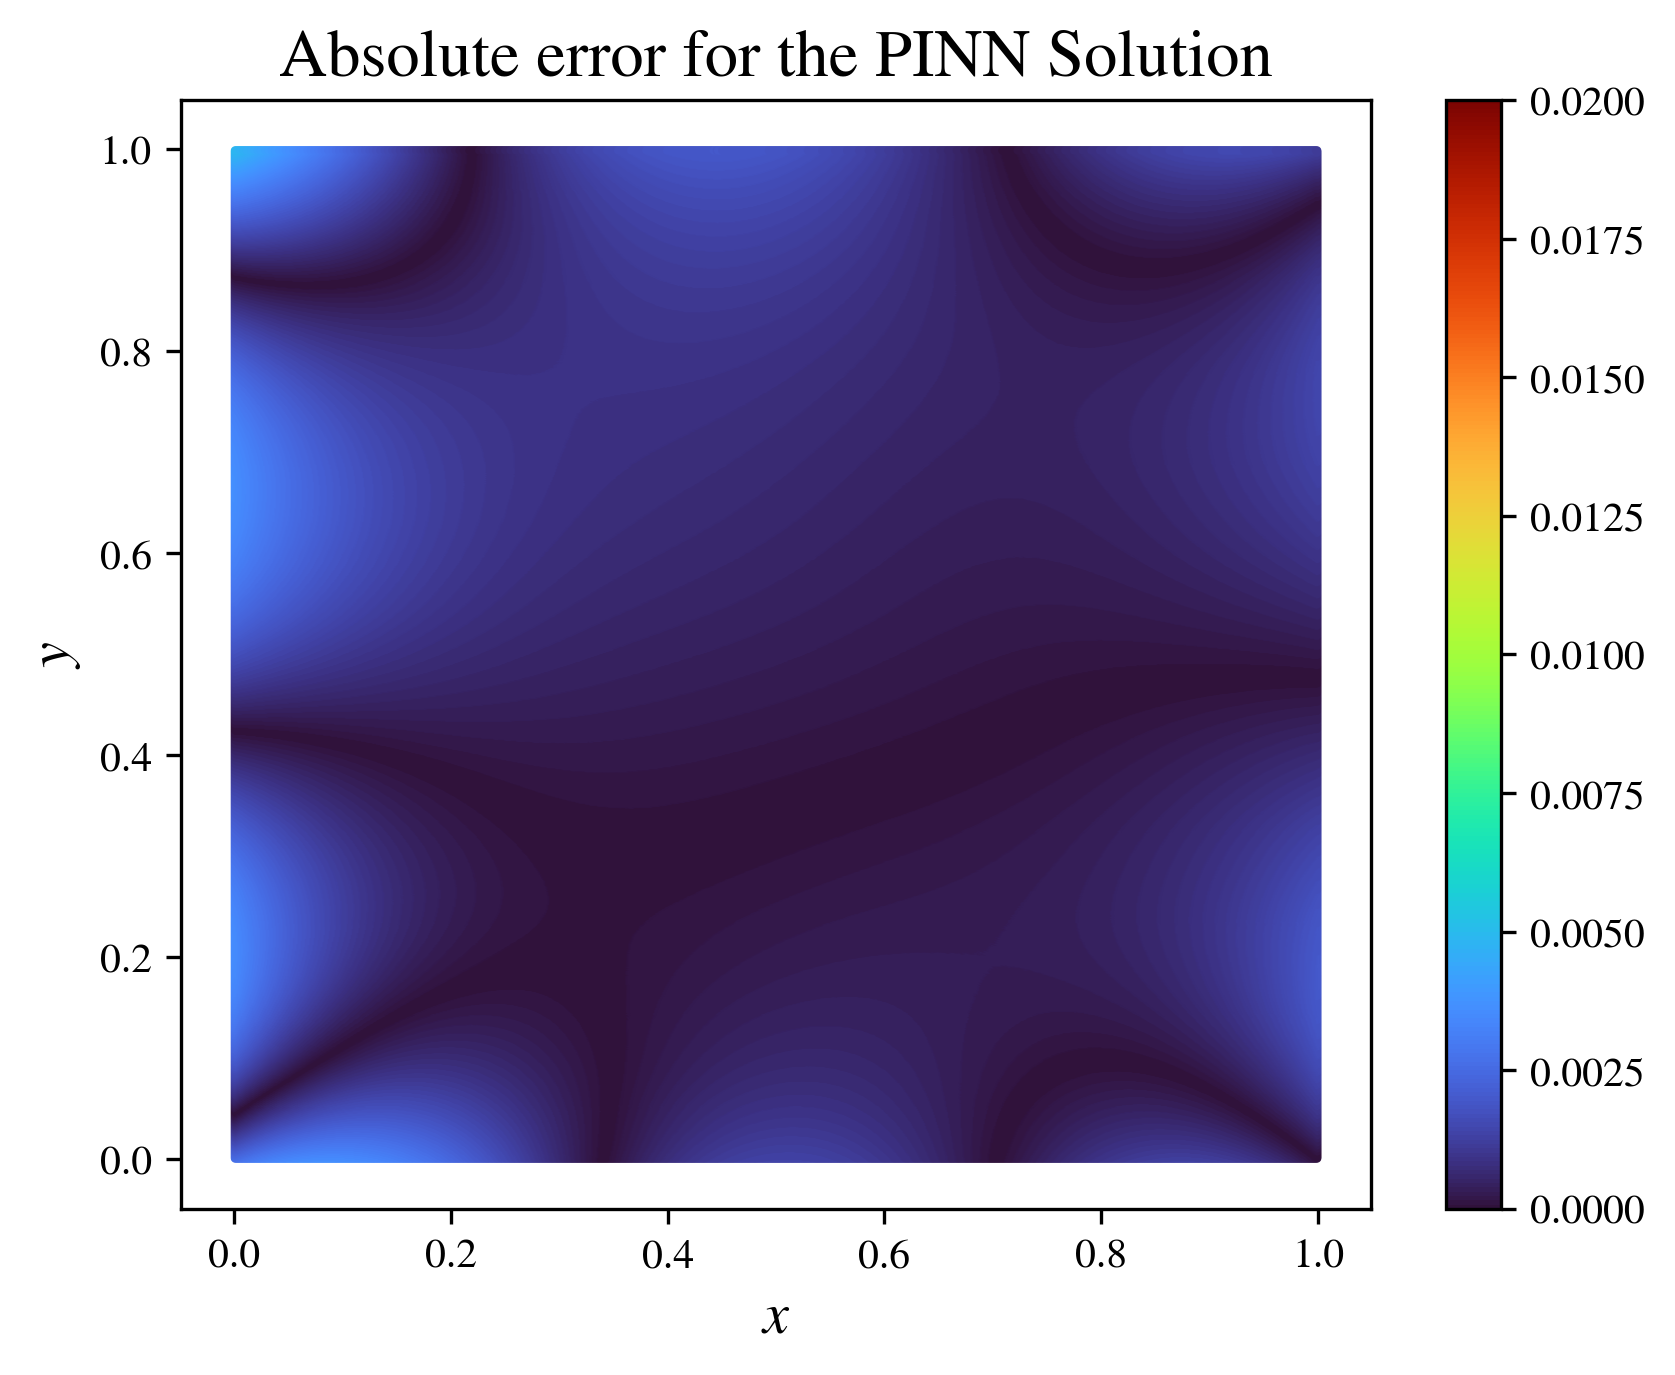
\includegraphics[width=\linewidth]{Project1XPINNs/figures/Poisson/smooth_single_Poisson_error.png}
    \caption{PINN absolute error with continuous residual.}
    \label{fig:pinn_smooth_error}
\end{figure}

\begin{figure}[h]
    \centering
    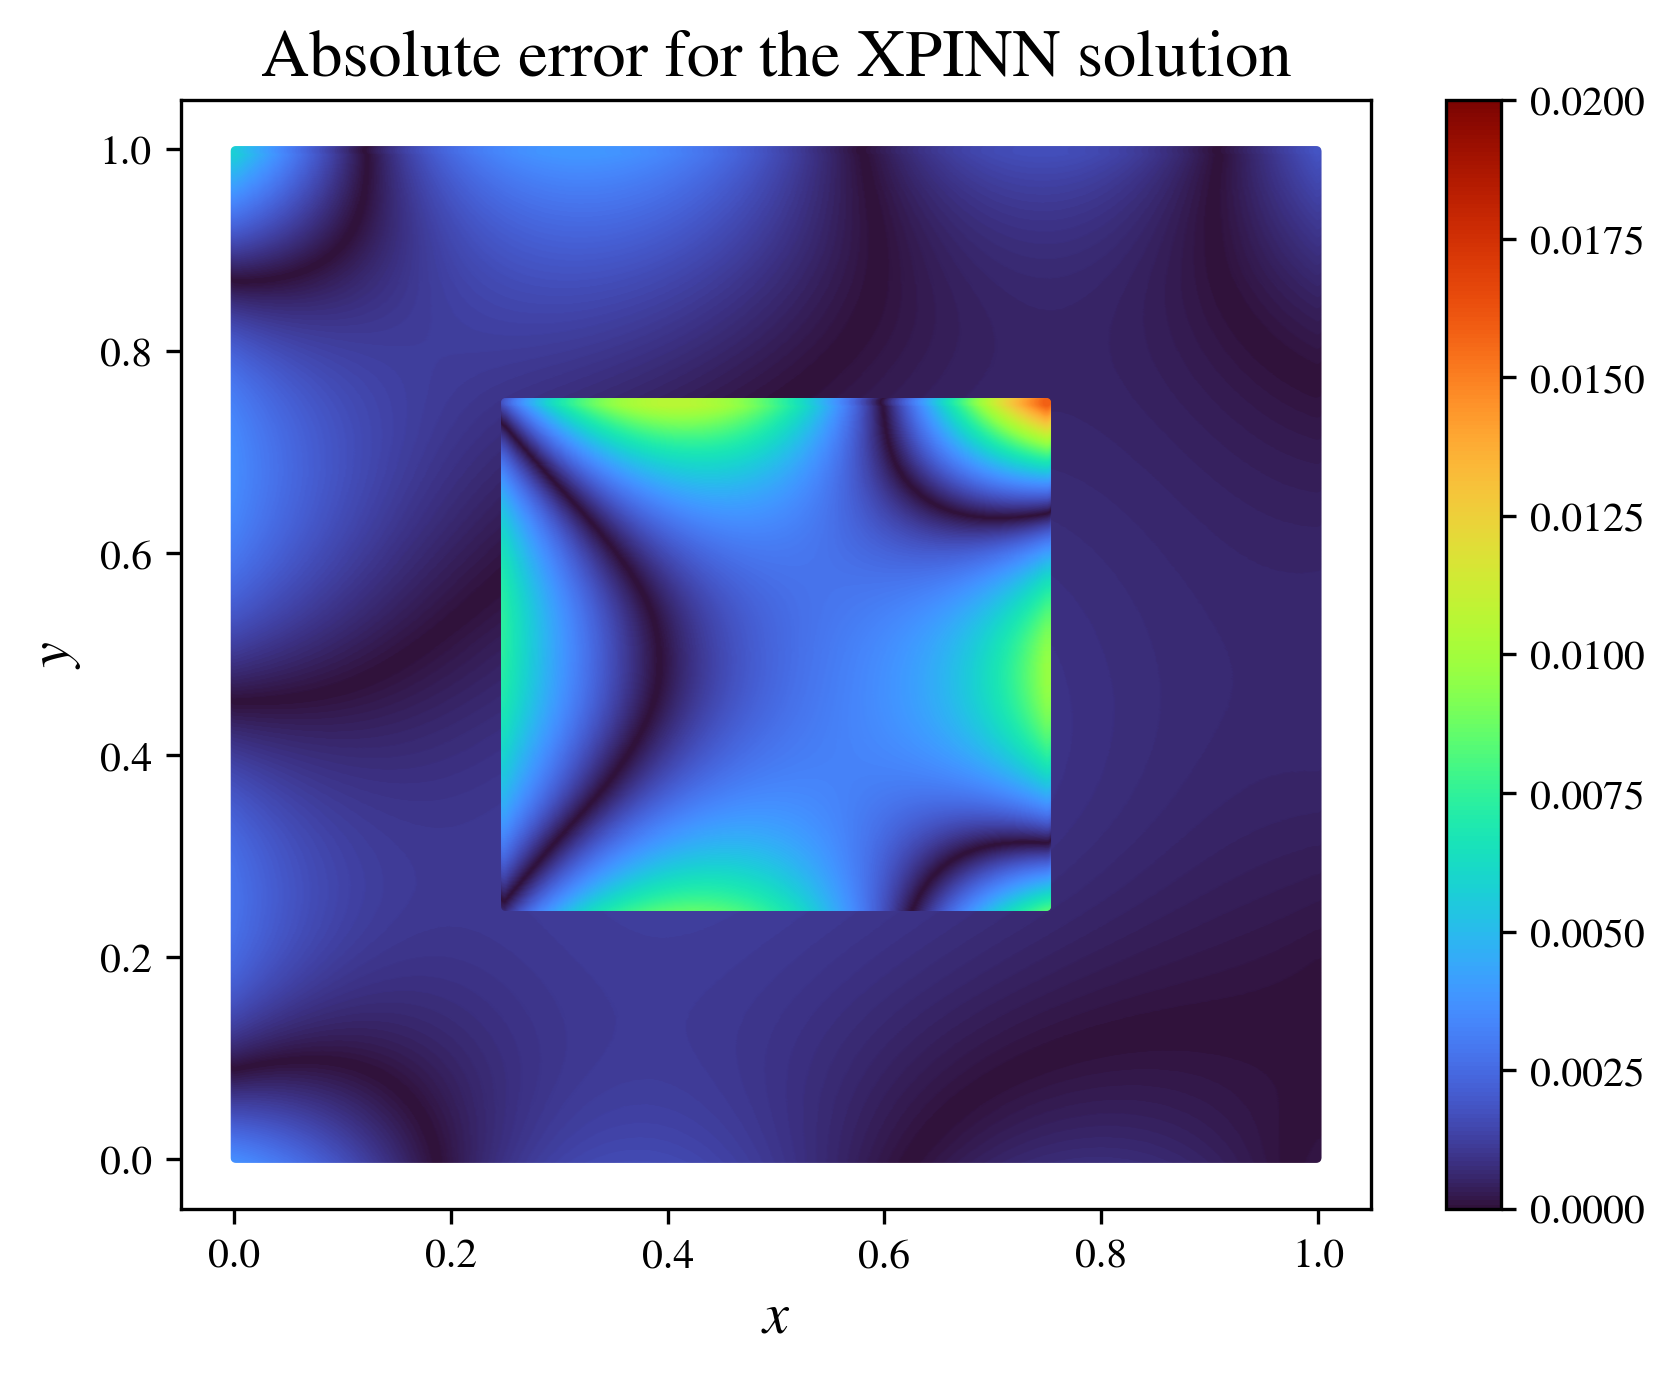
\includegraphics[width=\linewidth]{Project1XPINNs/figures/Poisson/smooth_xpinn_Poisson_error.png}
    \caption{XPINN absolute error with continuous residual.}
    \label{fig:xpinn_smooth_error}
\end{figure}

% \vfill\null

\paragraph{Discontinuous Residual:}
\autoref{fig:pinn_disc_pred} and \autoref{fig:xpinn_disc_pred} display the PINN and XPINN solutions.
Compared with the continuous residual, it is now much clearer where the subdomain boundaries are.
Interestingly, the outer sub-PINN visually looks similar to the solution of the PINN.
The error are shown in \autoref{fig:pinn_disc_error} and \autoref{fig:xpinn_disc_error}, this time with different colorbars as the maximum error of the XPINN is significantly higher than that of the PINN.
Both solvers seem to perform worse on this problem. Notably, the XPINN solver appears to perform significantly worse, which is according to expectations \cite{XPINN_generalize}.

\begin{figure}[h]
    \centering
    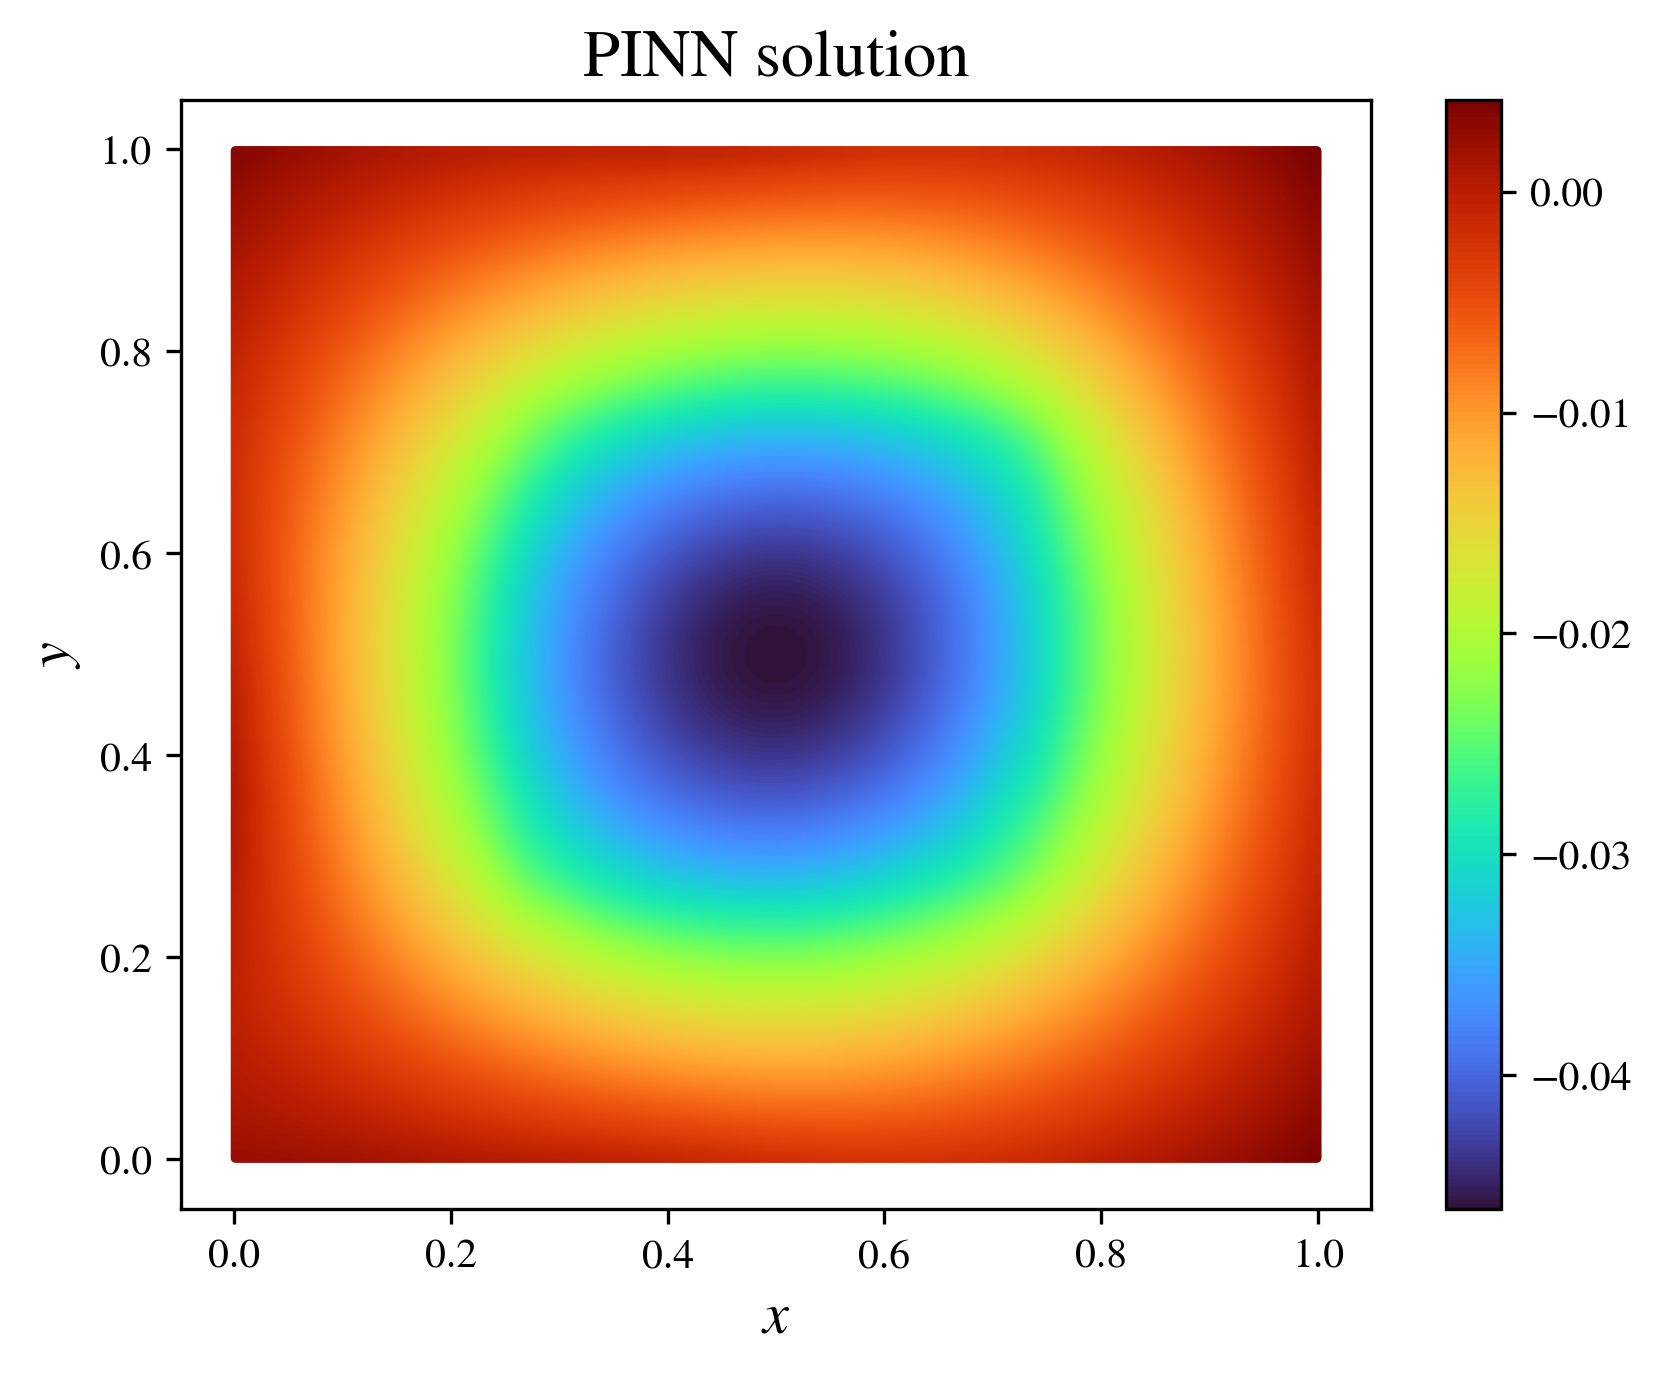
\includegraphics[width=\linewidth]{Project1XPINNs/figures/Poisson/discrete_single_Poisson_solution.pdf.png}
    \caption{PINN prediction with discontinuous residual.}
    \label{fig:pinn_disc_pred}
\end{figure}

\begin{figure}[h]
    \centering
    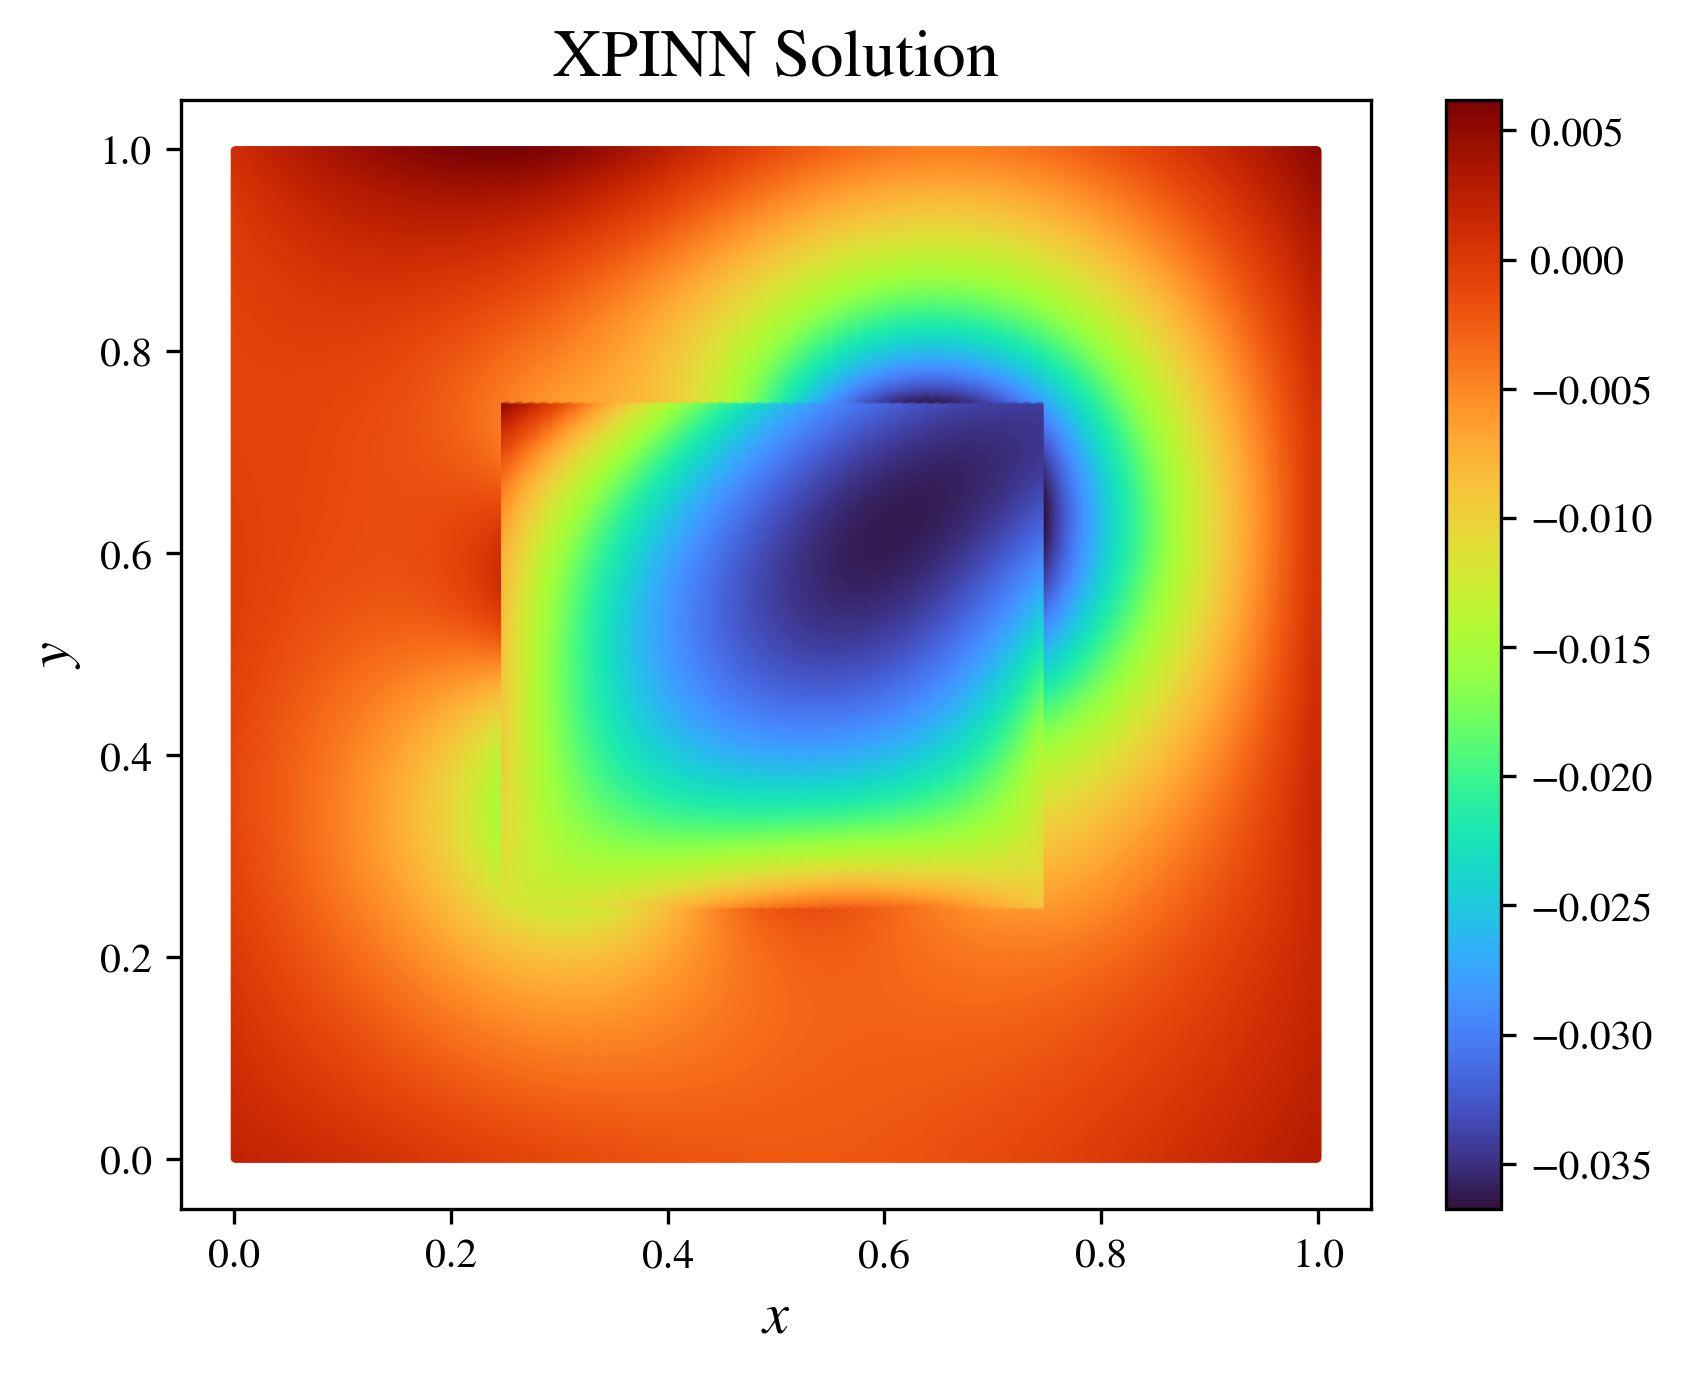
\includegraphics[width=\linewidth]{Project1XPINNs/figures/Poisson/new_exp/discrete_xpinn_Poisson_solution.png}
    \caption{XPINN prediction with continuous residual.}
    \label{fig:xpinn_disc_pred}
\end{figure}

\begin{figure}[h]
    \centering
    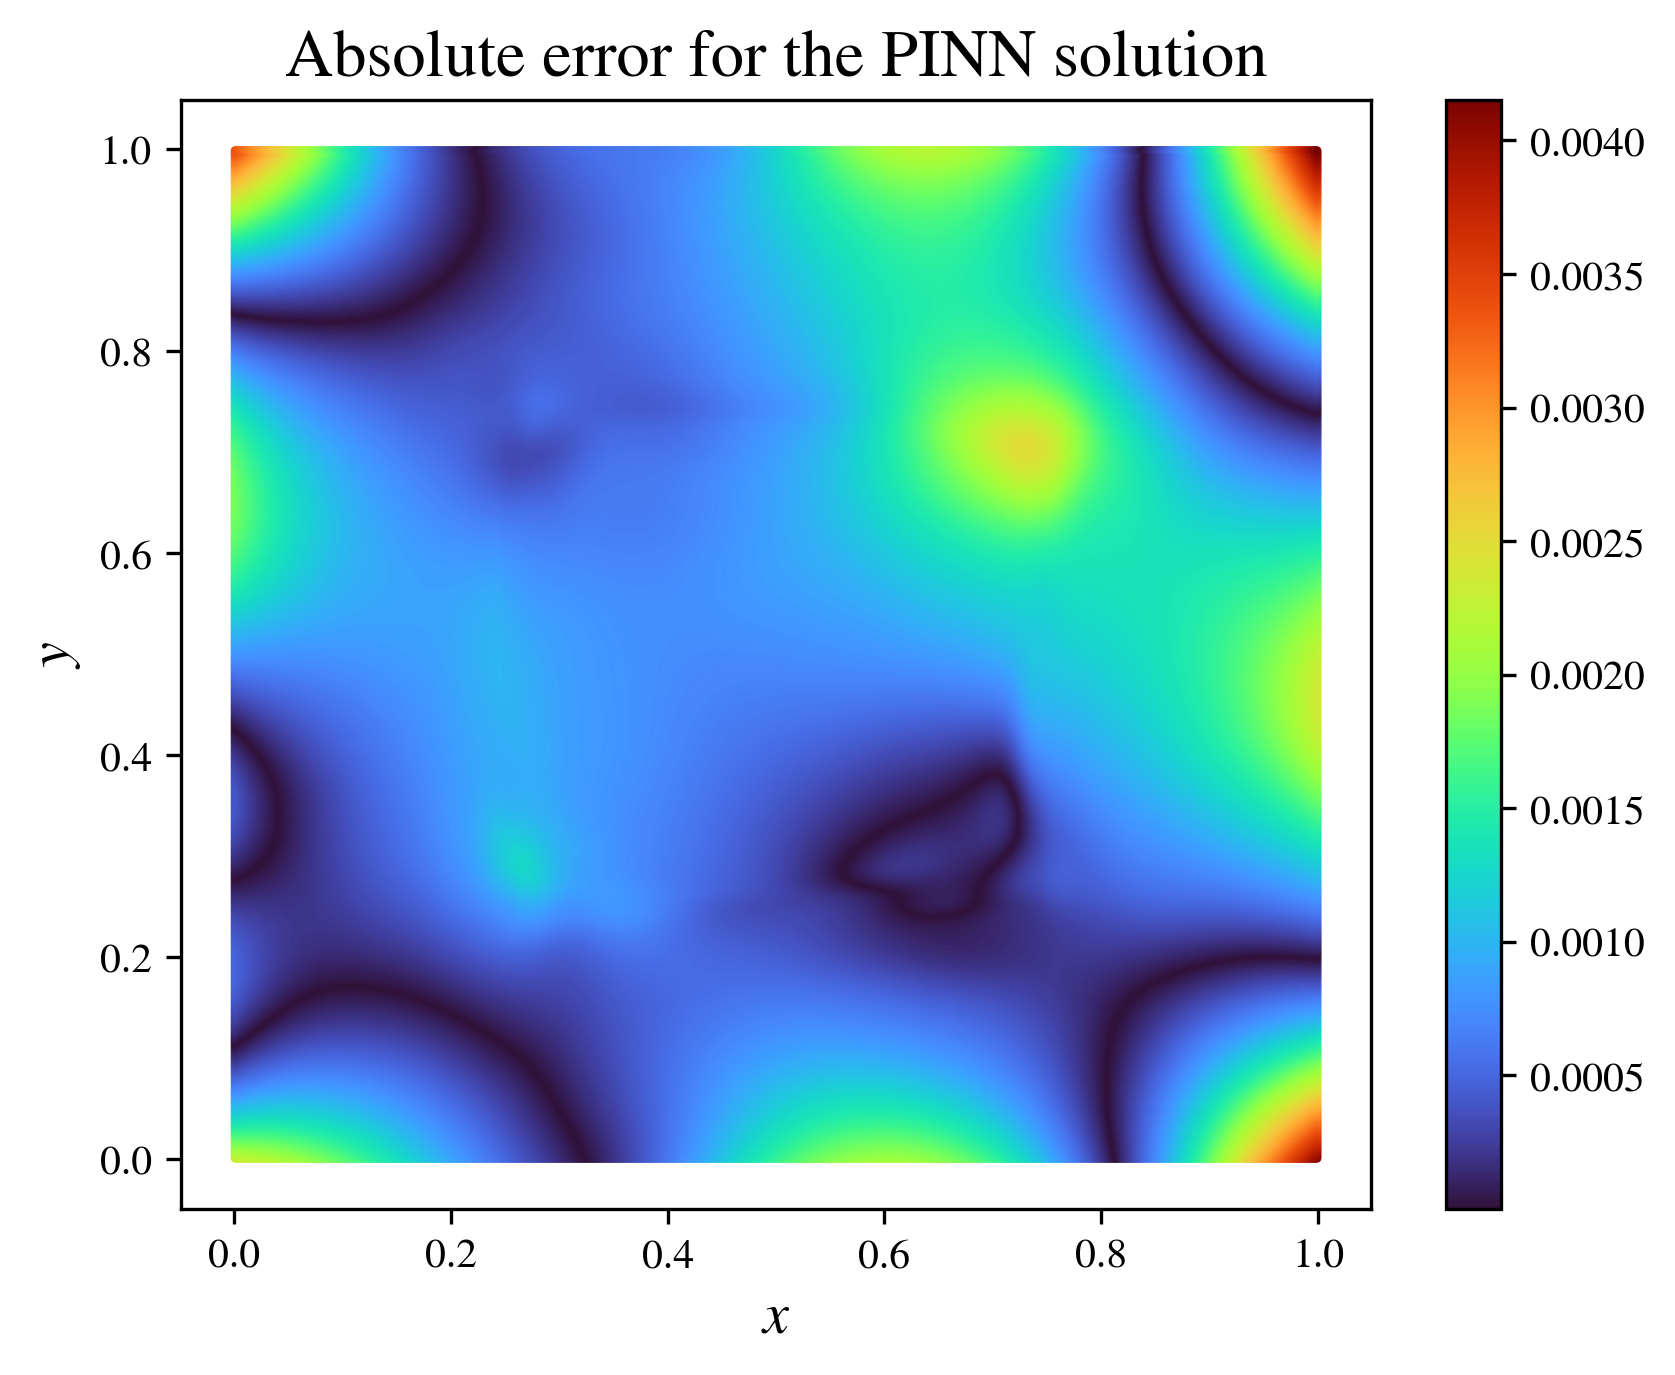
\includegraphics[width=\linewidth]{Project1XPINNs/figures/Poisson/discrete_single_Poisson_error.pdf.png}
    \caption{PINN absolute error with discontinuous residual.}
    \label{fig:pinn_disc_error}
\end{figure}

\begin{figure}[h]
    \centering
    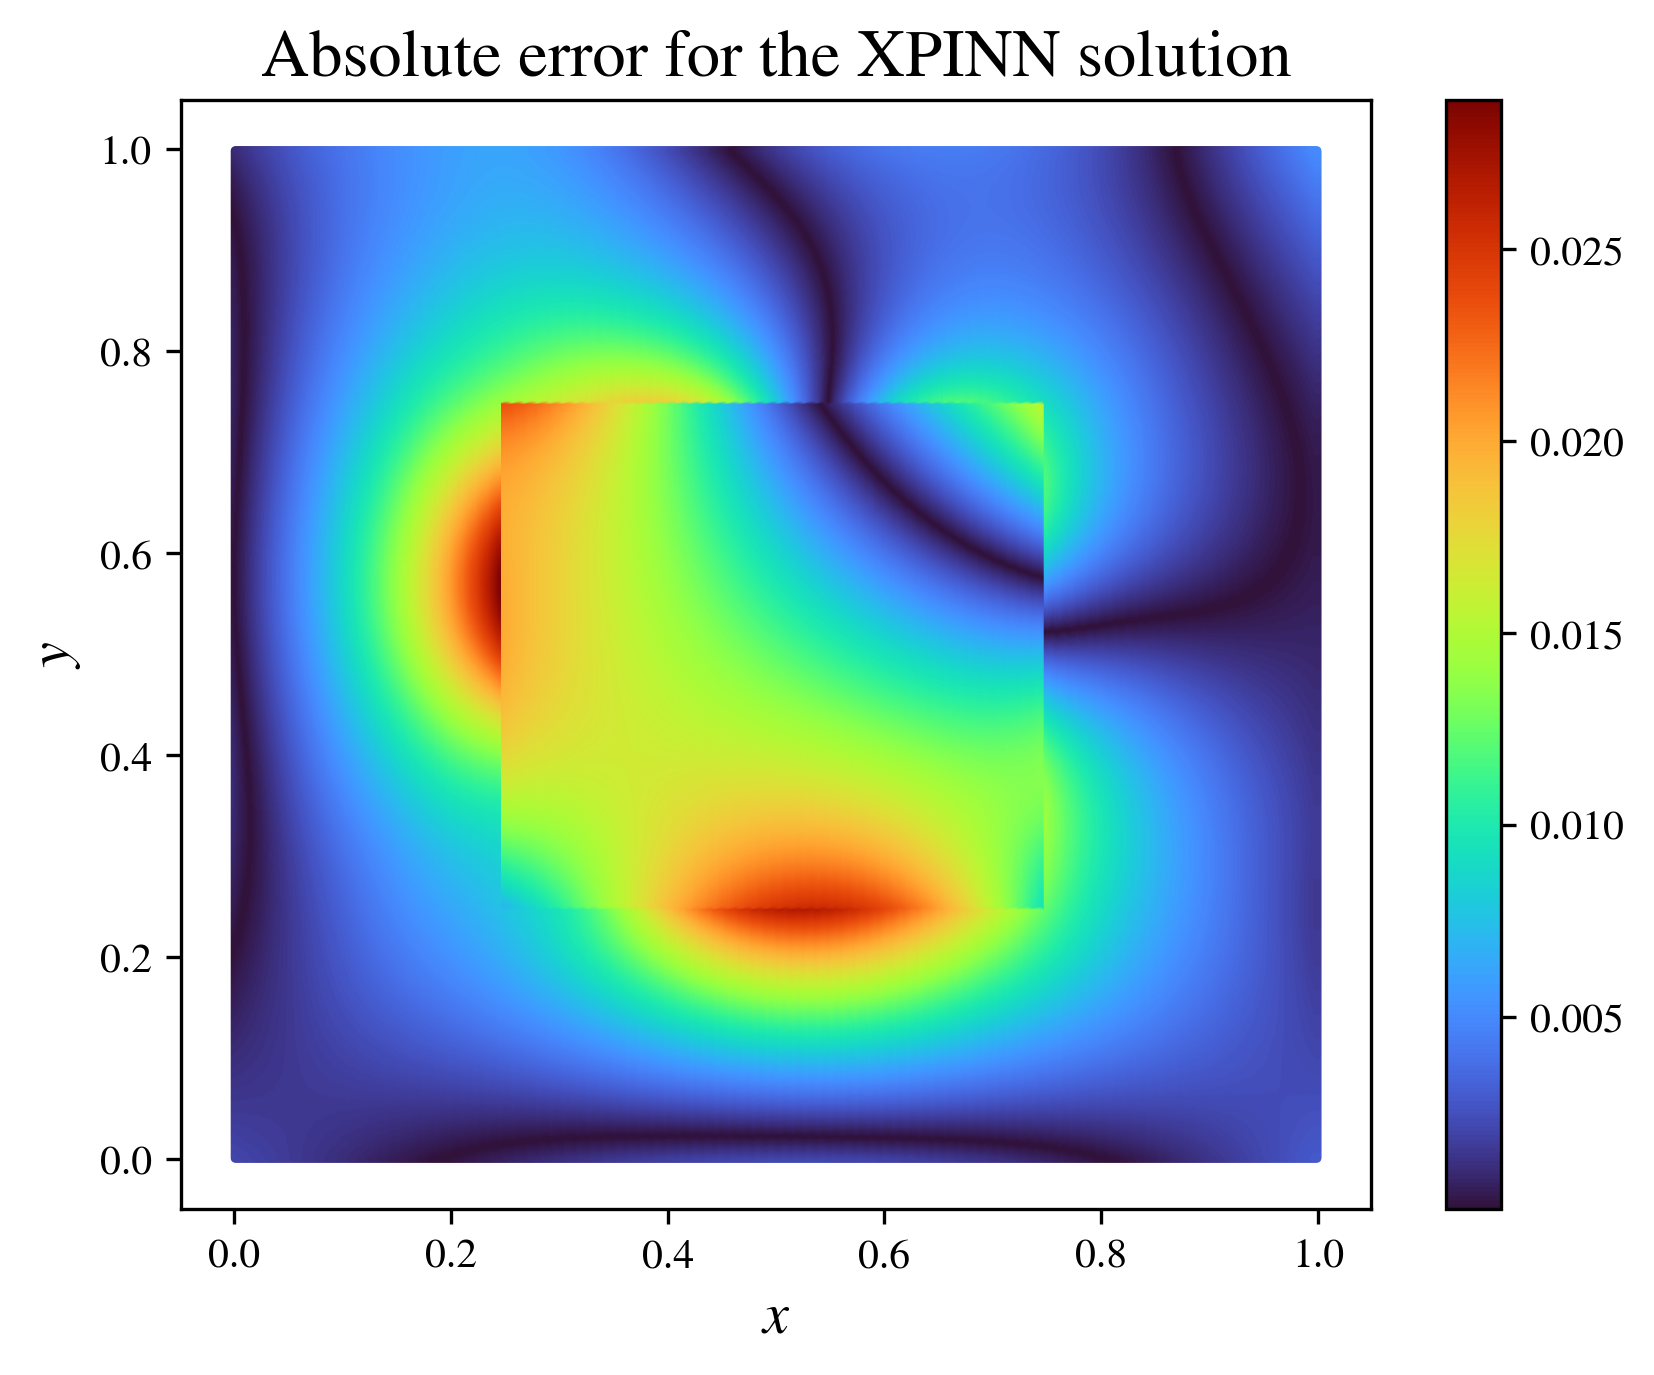
\includegraphics[width=\linewidth]{Project1XPINNs/figures/Poisson/new_exp/discrete_xpinn_Poisson_error.png}
    \caption{XPINN absolute error with discontinuous residual.}
    \label{fig:xpinn_disc_error}
\end{figure}

Wondering whether this discrepancy is due a lack of training, we investigated the loss per epoch, shown in \autoref{fig:xpinn_disc_loss}.
As we see, the loss only sees marginal improvements after 125 000 iterations.
The same is seen with the relative $L^2$ error in \autoref{fig:rel_l2_discrete_poisson}, wherein the PINNs stabilize, while the XPINNs remains higher.
We therefore believe this is partly due to the reduced number of training points.
The points are drawn from a uniform distribution, and as the center subdomain is $[0.25, 0.75] \times [0.25, 0.75]$, it receives on average just $25\%$ of the total points.
In addition, given the symmetric nature of the problem, one can argue for whether evenly spaced points might outperform our choice of uniformly random points.

The relative $L^2$ errors are also summarized in \autoref{table:discont_poisson}.
The XPINNs give a median error about an order of magnitude higher than that of the PINN over 10 runs.
These results are consistent with what was found in \cite{XPINN_generalize}.

\begin{figure}[h]
    \centering
    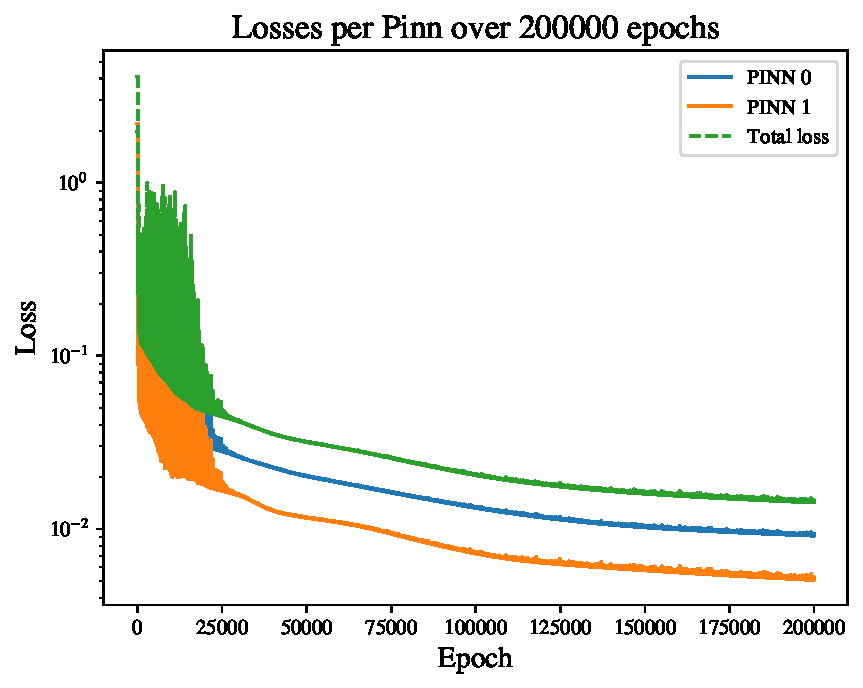
\includegraphics[width=\linewidth]{Project1XPINNs/figures/Poisson/new_exp/discrete_xpinn_Poisson_losses.pdf}
    \caption{Loss per epoch for XPINN on the Poisson equation with discontinuous residual.}
    \label{fig:xpinn_disc_loss}
\end{figure}
\begin{figure}[h!]
    \centering
    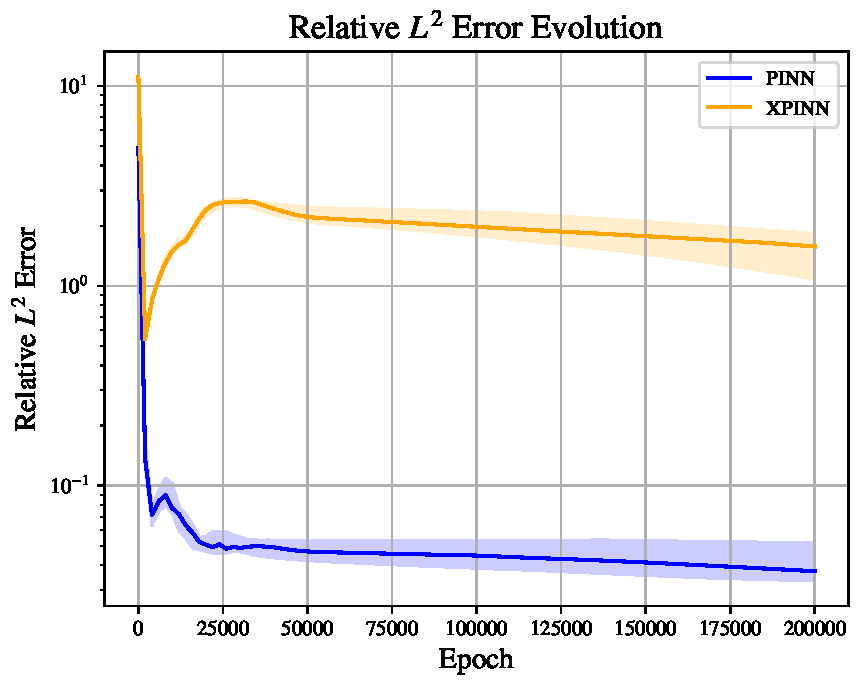
\includegraphics[width = \linewidth]{Project1XPINNs/figures/Poisson/discrete_l2_error_evolution.pdf}
    \caption{Relative $L^2$ error with median and interquartile range highlighted, for PINN and XPINN with discontinuous residual.}
    \label{fig:rel_l2_discrete_poisson}
\end{figure}

\begin{table}[h!]
\caption{Median, minimum and maximum of the relative $L^2$-errors for the Poisson equation with discontinuous residual achieved by the PINN and XPINN.}
\centering
\begin{tabular}{r|c|c|c}\toprule
     & Median & Minimum & Maximum \\
    \colrule
    PINN & $3.73 \cdot 10^{-2}$ & $3.11 \cdot 10^{-2}$ & $6.05 \cdot 10^{-2}$ \\
    XPINN & $4.69 \cdot 10^{-1} $ &  $2.36 \cdot 10^{-1}$ & $1.00 \cdot 10^{0}$ \\
    \botrule
\end{tabular}
\label{table:discont_poisson}
% \vspace{-0.5cm}
\end{table}
\vfill\null

\subsection{Navier-Stokes Equation}
\subsubsection{Problem Formulation}
Finally, we consider the steady Navier-Stokes equation at Reynolds number $Re = 20$ as described in the FEATFLOW benchmark suite \cite{DFG}.
The problem is a simulation of incompressible 2D fluid flow past a cylinder in a rectangular domain.
The steady, incompressible Navier Stokes equation can be written as
\begin{equation}\label{eq:NS}
    -\nu \nabla^2 \mathbf{u} + (\mathbf{u} \cdot \nabla)\mathbf{u} + \nabla p = \mathbf{0}, \quad \nabla \cdot \mathbf{u} = 0,
\end{equation}
where $\nu = 0.001$.
In our notation, we will isolate the $x$- and $y$-flow as $u$ and $v$ respectively, writing $\mathbf{u} = (u,v)^\intercal$.
From this, we can express the PDEs for the second-order spatial derivatives, as well as the equation for zero convergence due to incompressibility as
\begin{equation}
\begin{cases}
-\nu(u_{xx} + u_{yy})+uu_x+vu_y+p_x = 0, \\
-\nu(v_{xx} + v_{yy})+uv_x+vv_y+p_y = 0, \\
u_x + v_y = 0.
\end{cases}
\end{equation}
The domain of the problem is given by % \vspace{-1mm}
\begin{align*}
    \Omega = [0,2.2] \times [0,0.41] \setminus B_r(0.2,0.2), \hspace{4mm} r = 0.05.
\end{align*}

In order to impose the zero divergence condition, we consider the stream function $\psi$ characterizing incompressible flow. $u$ and $v$ can then be obtained through $u=\psi_y$ and $v=-\psi_x$. Our network $\mathcal{N}_\theta$ thus predicts the stream function $\psi$ and the pressure $p$, with
\begin{equation}
    \mathcal{N}_\theta : \mathbb{R}^2 \to \mathbb{R}^2, \quad (x,y)\to (\psi, p).
\end{equation}


This problem includes three different boundary conditions.
First, we have the boundary for the upper and lower walls, as well as around the edge of the cylinder.
In the DFG benchmark 2D-1 \cite{DFG}, the lower and upper walls are notated as $\Gamma_1 = [0,2.2]\times 0$ and $\Gamma_3 = [0,2.2]\times 0.41$ respectively, and the cylinder as $S=\partial B_r(0.2,0.2)$.
On these walls, we enforce impermeability and the no-slip conditions, leading to zero-flow on these boundaries. 
The no-slip boundary condition is defined as
\begin{equation}
\begin{split}
    u_{|\Gamma_1} = u_{|\Gamma_3} &= u_{|S} = 0, \\
    v_{|\Gamma_1} = v_{|\Gamma_3} &= v_{|S} = 0.
\end{split}
\end{equation}
On the left boundary we enforce polynomial inflow.
The left boundary is $\Gamma_2 = 0\times [0,0.41]$ and the polynomial inflow is given by
\begin{equation}
    u=\frac{4Uy(0.41-y)}{0.41^2}, \quad v=0,
\end{equation}
where $U=0.3$, and the mean inlet velocity  is $U_{\text{mean}} = 0.2$.
Finally, on the right boundary we have the do-nothing boundary condition.
The boundary is $\Gamma_4=2.2\times[0,0.41]$, and the condition is given by
\begin{equation}
    \nu u_x - p = 0, \quad \nu u_y = 0.
\end{equation}
Hence, we confirm our target Reynolds number using the cylinder diameter as the characteristic length $L=0.1$.
$U_{\text{mean}}$ is used as the characteristic velocity.
The Reynolds number then becomes
\begin{equation}
    Re = \frac {U_{\text{mean}} L} \nu = \frac {0.2 \cdot 0.1} {0.001} = 20.
\end{equation}

\subsubsection{Results}
Achieving qualitative results required a fair deal of hyperparameter tuning, especially the weighting of the losses in \eqref{eq:PINNMSE}, as well as the model architecture.
This search was not carried out exhaustively, but rather through a heuristic approach of trial and error.
Given this, it should be recognized that there may still be potential to achieve better results.

The PINN was structured with 25 hidden layers, each consisting of 30 nodes, with the $\tanh$ activation function and unitary weighting of the loss function.
We utilized exponential decay in order to tune the learning rate of \textsc{Adam}, leading to a rapid, chaotic, decrease in the measured loss in the early epochs, stabilizing, as in \autoref{fig:NS_PINN_losses}.
The loss did not fully plateau, meaning there could be room for improvement, although that might also be indicative of overfitting.

\begin{figure}[th]
    \centering
    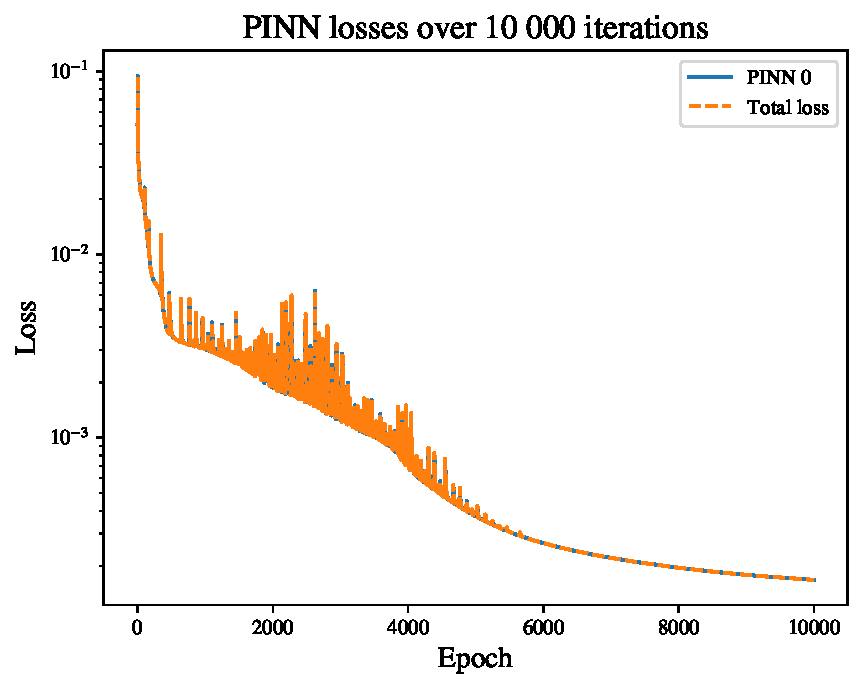
\includegraphics[width=\linewidth]{Project1XPINNs/figures/NavierStokes/NoDecomp/ND_10000_iter_30x25/losses/PINN_losses.pdf}
    \caption{Loss per epoch for PINN on the Navier-Stokes equation.}
    \label{fig:NS_PINN_losses}
\end{figure}

The domain decomposition for the XPINN consisted of
\begin{equation}
    \Omega_2 = [0.8, 2.2] \times [0, 0.41] \quad\text{and}\quad
    \Omega_1 = \Omega \setminus \Omega_2.
\end{equation}
The XPINN was structured with 25 hidden layers nodes for $\Omega_1$ and 10 hidden layers for $\Omega_2$, all with 30 nodes each.
As the XPINN encountered difficulties on the interface, we imposed Neumann interface condition on $\psi$ in order to increase performance.
This involved including a continuity loss on the flow field, with
\begin{align}
    \frac{1}{N_I} \sum_{i=0}^{N_I} \left( \nabla \psi(x_I^i) - \{ \nabla\psi_I^i \}  \right)^2,
\end{align}
where $\{\nabla\psi_I^i\}$ is the average gradient predicted at the interface, allegoric to \eqref{eq:MSE_I}.

The loss for the XPINN seems to stabilize earlier in \autoref{fig:NS_XPINN_losses}, although do note that the loss is not directly comparable with \autoref{fig:NS_PINN_losses}, as in addition to the Neumann interface condition, we applied a heavy weighting of 20 on the inflow boundary, and a weighting of 40 on the left-to-right interface.
Even with this weighting, the interface is still clearly visible in \autoref{fig:NS_XPINN_flow_mag}.
To further enhance performance at the interface, we could explore additional adjustments, such as introducing more continuity conditions, e.g. Robin continuity.

\begin{figure}[h]
    \centering
    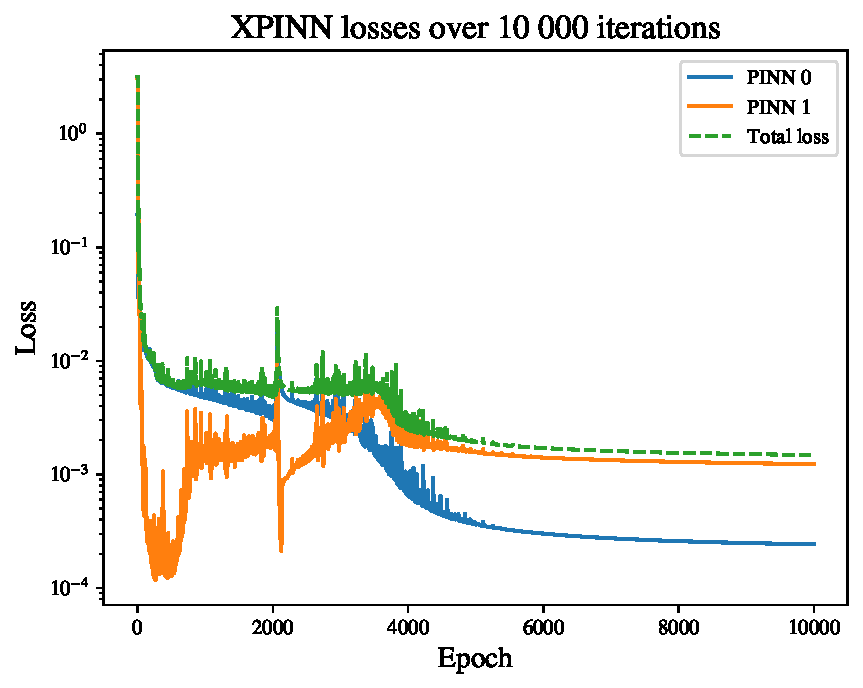
\includegraphics[width=\linewidth]{Project1XPINNs/figures/NavierStokes/TwoBoxDecomp/TB_10000_iter_right_emphasis/losses/TwoBox_decomp_losses.pdf}
    \caption{Loss per epoch for XPINN on the Navier-Stokes equation.}
    \label{fig:NS_XPINN_losses}
\end{figure}

In general, the PINN produced better results than the XPINN.
However, with the reduced complexity of the XPINN, we were able to increase the computational speed significantly.
Having said that, both our models successfully replicated the flow plots from the DFG benchmark  \cite{DFG}, as illustrated in Figures \ref{fig:NS_PINN_FlowMag} through \ref{fig:NS_XPINN_streamfunc}.
It should be noted on comparison with the benchmark that slightly different colorings were used.

\begin{figure}[h]
    \centering
    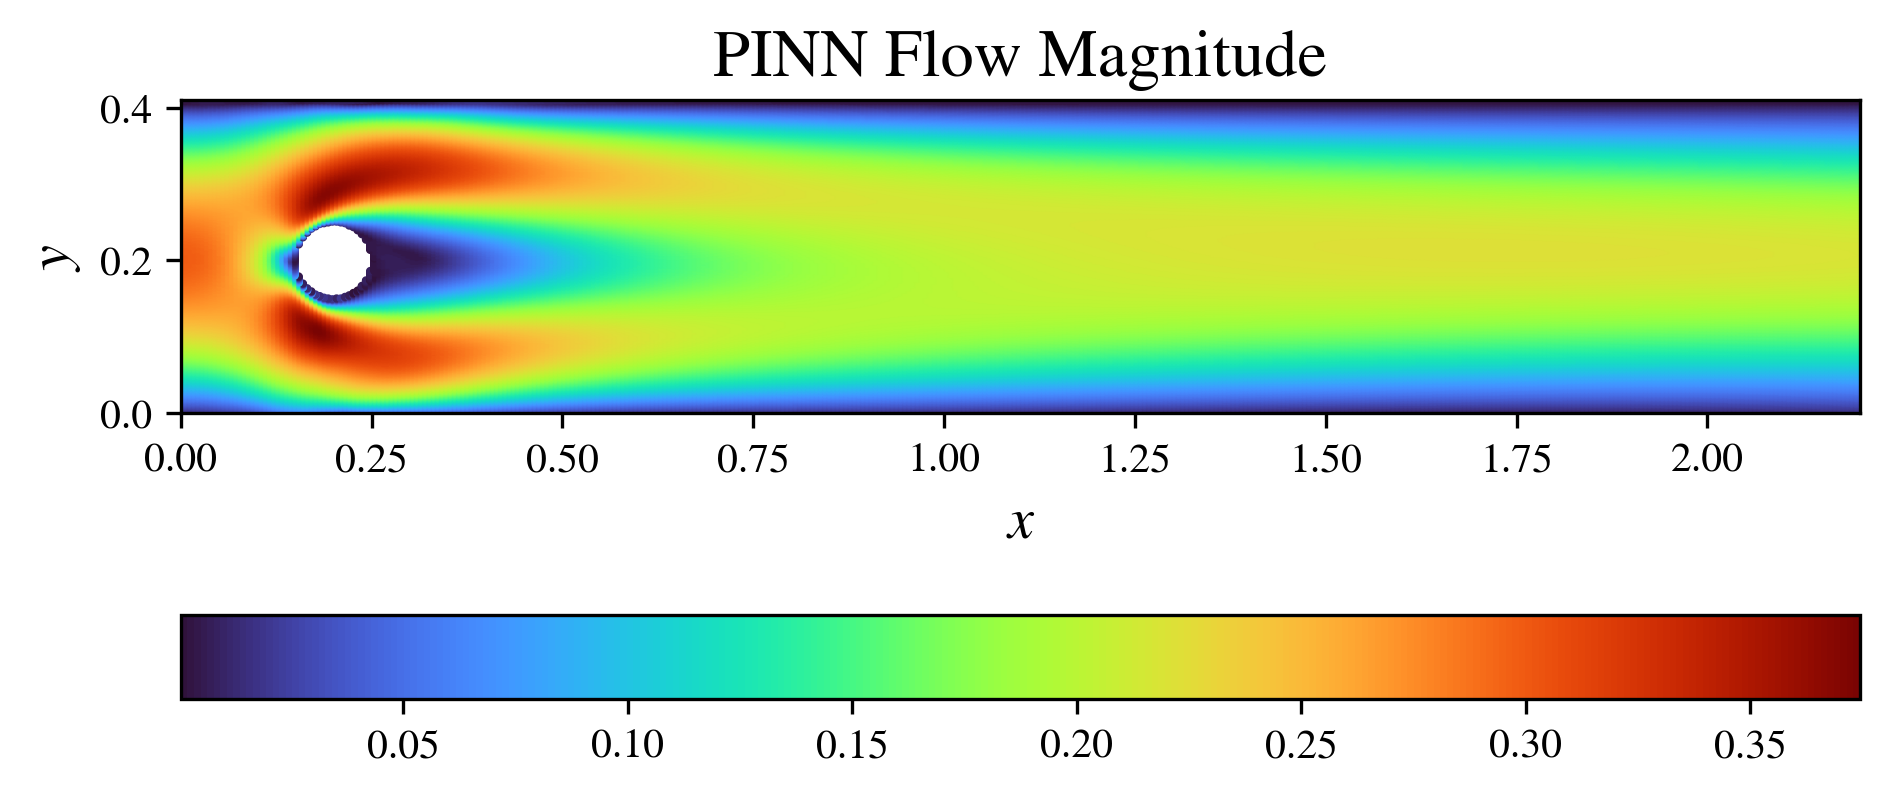
\includegraphics[width=\linewidth]{Project1XPINNs/figures/NavierStokes/NoDecomp/ND_10000_iter_30x25/solution/flow_magnitude_no_decomp.png}
    \caption{Velocity magnitude of the PINN.}
    \label{fig:NS_PINN_FlowMag}
\end{figure}

\begin{figure}[h]
    \centering
    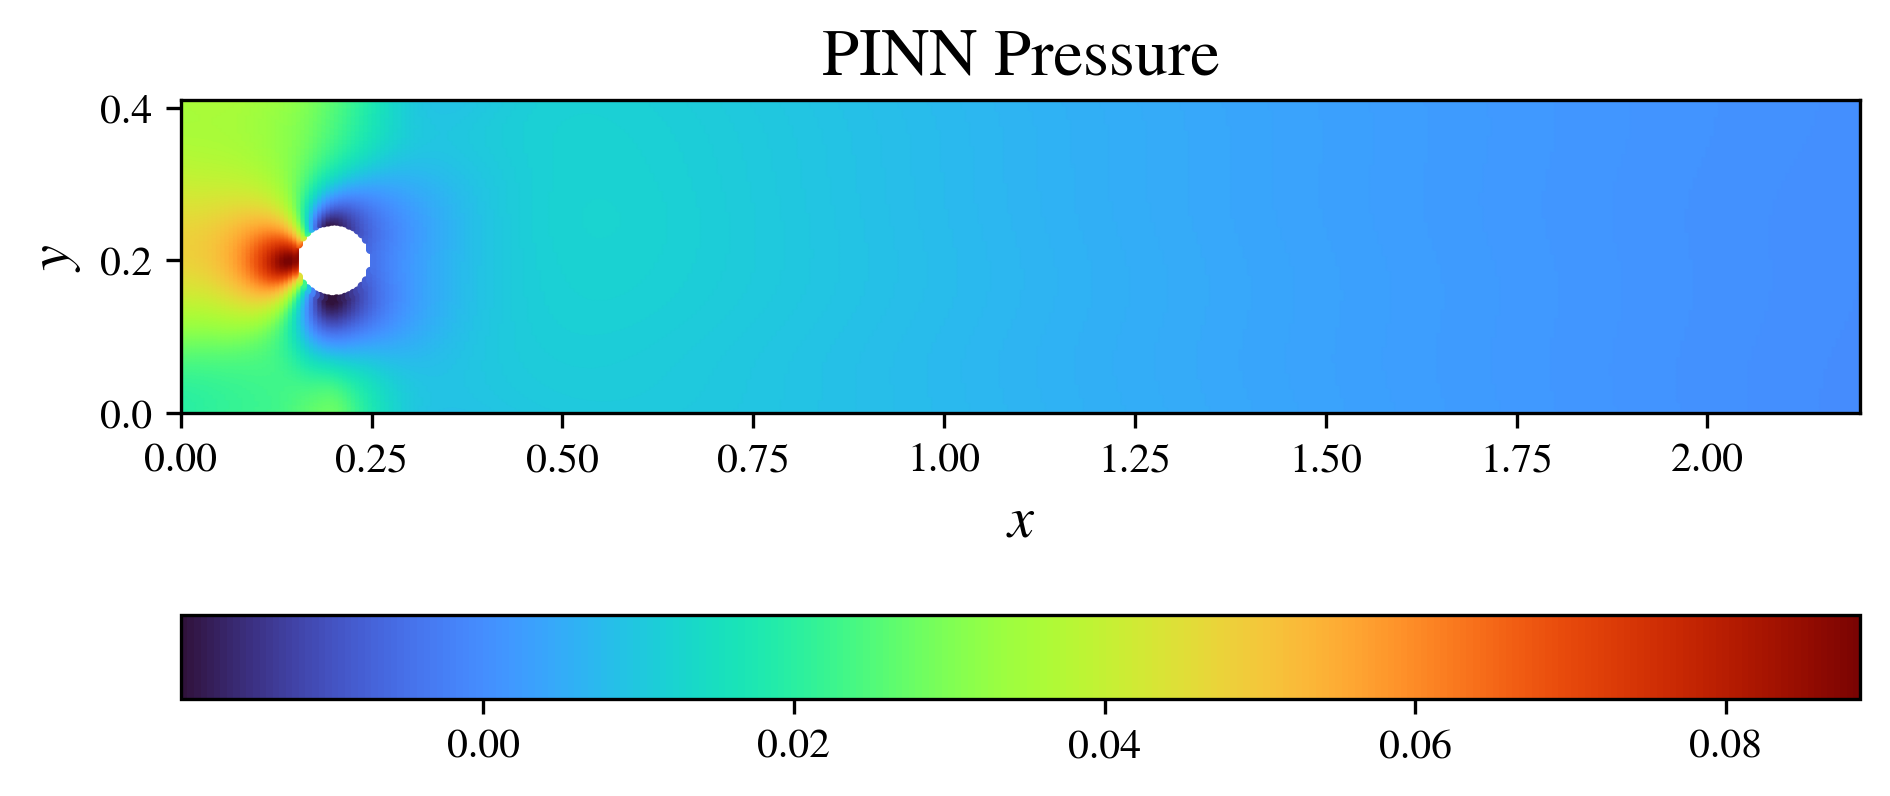
\includegraphics[width=\linewidth]{Project1XPINNs/figures/NavierStokes/NoDecomp/ND_10000_iter_30x25/solution/pressure_no_decomp.png}
    \caption{Pressure prediction of the PINN.}
    \label{fig:NS_PINN_Pressure}
\end{figure}

\begin{figure}[h]
    \centering
    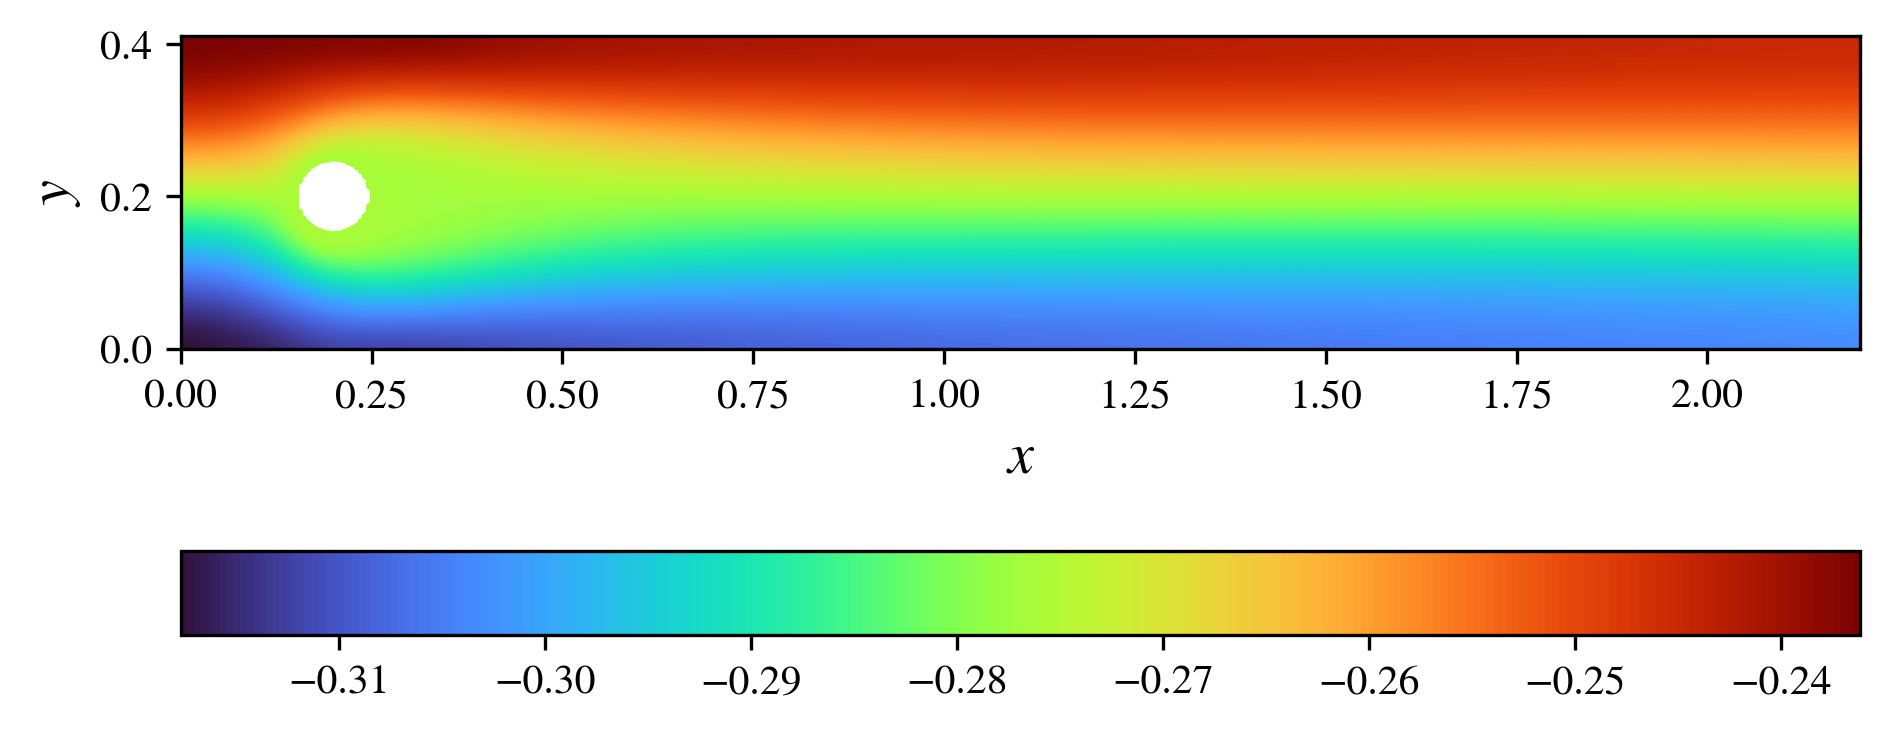
\includegraphics[width=\linewidth]{Project1XPINNs/figures/NavierStokes/NoDecomp/ND_10000_iter_30x25/solution/streamfunc_no_decomp.png}
    \caption{Predicted streamfunction of the PINN.}
    \label{fig:NS_PINN_Streamfunc}
\end{figure}

\begin{figure}[h!]
    \centering
    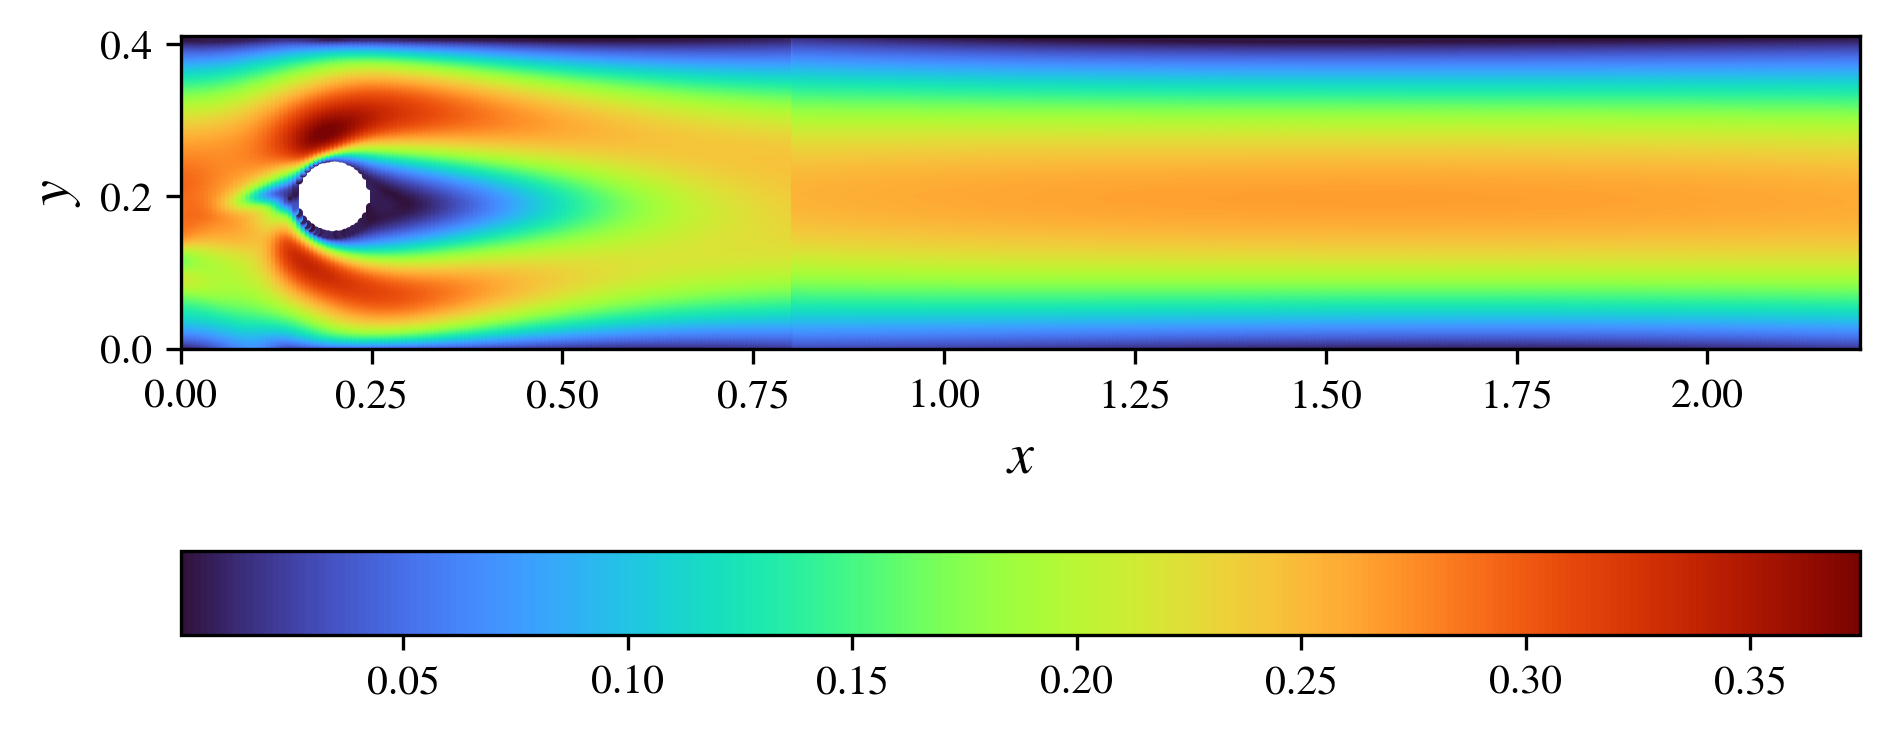
\includegraphics[width=\linewidth]{Project1XPINNs/figures/NavierStokes/TwoBoxDecomp/TB_10000_iter_right_emphasis/solution/flow_magnitude_two_box.png}
    \caption{Velocity magnitude of the XPINN.}
    \label{fig:NS_XPINN_flow_mag}
\end{figure}

\begin{figure}[h!]
    \centering
    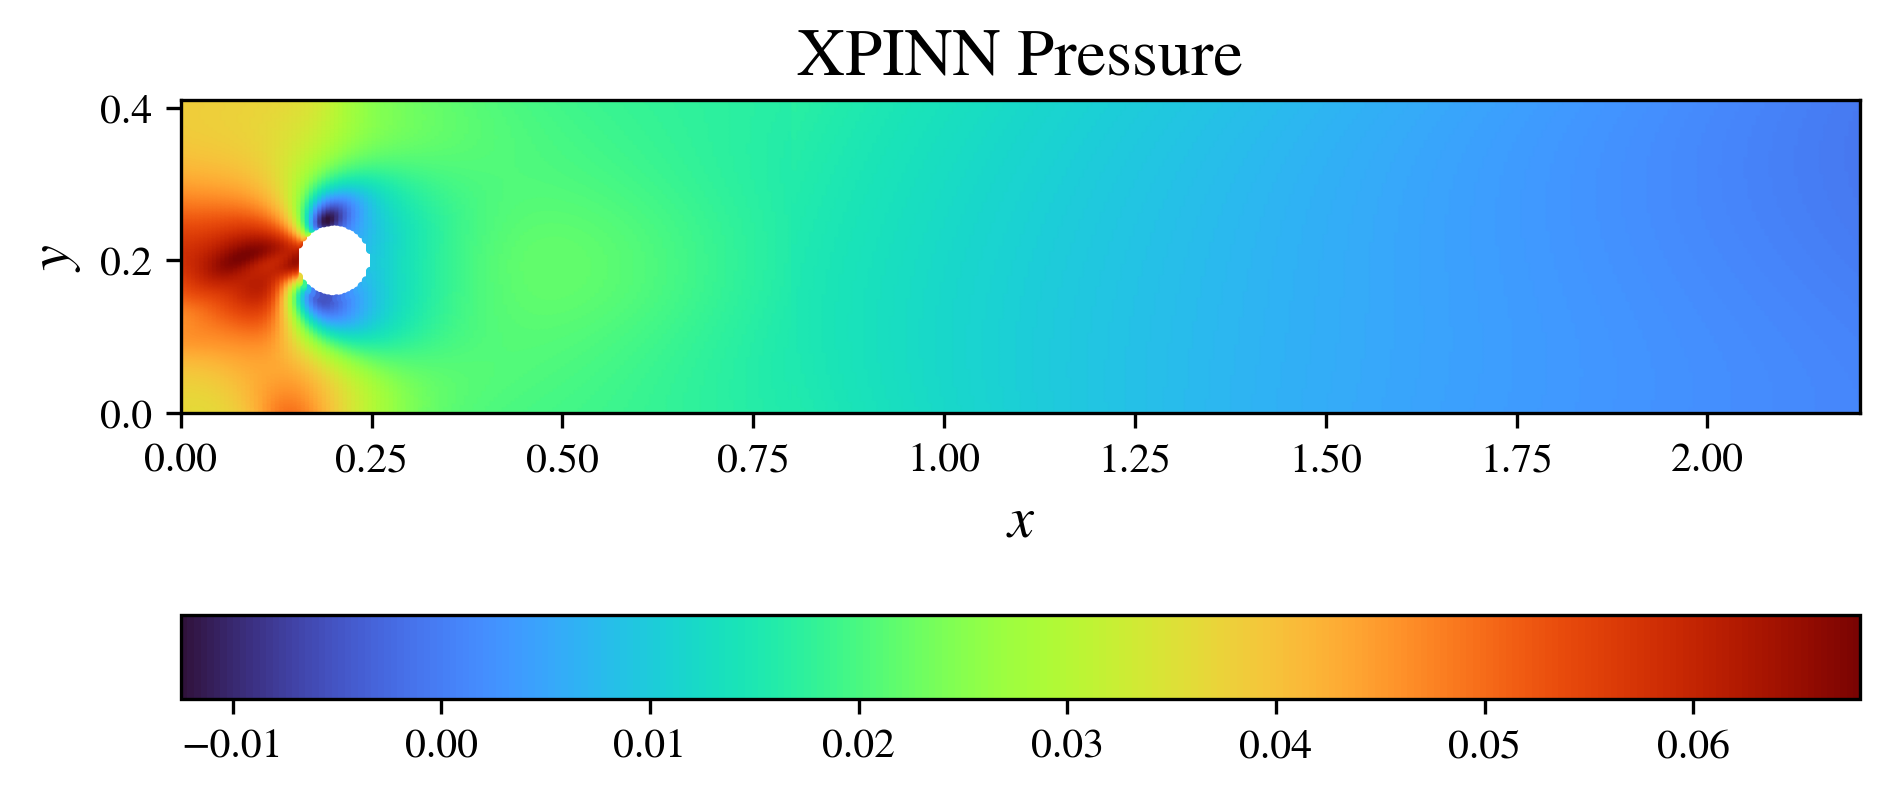
\includegraphics[width=\linewidth]{Project1XPINNs/figures/NavierStokes/TwoBoxDecomp/TB_10000_iter_right_emphasis/solution/pressure_two_box.png}
    \caption{Predicted pressure of the XPINN.}
    \label{fig:NS_XPINN_pressure}
\end{figure}

\begin{figure}[h!]
    \centering
    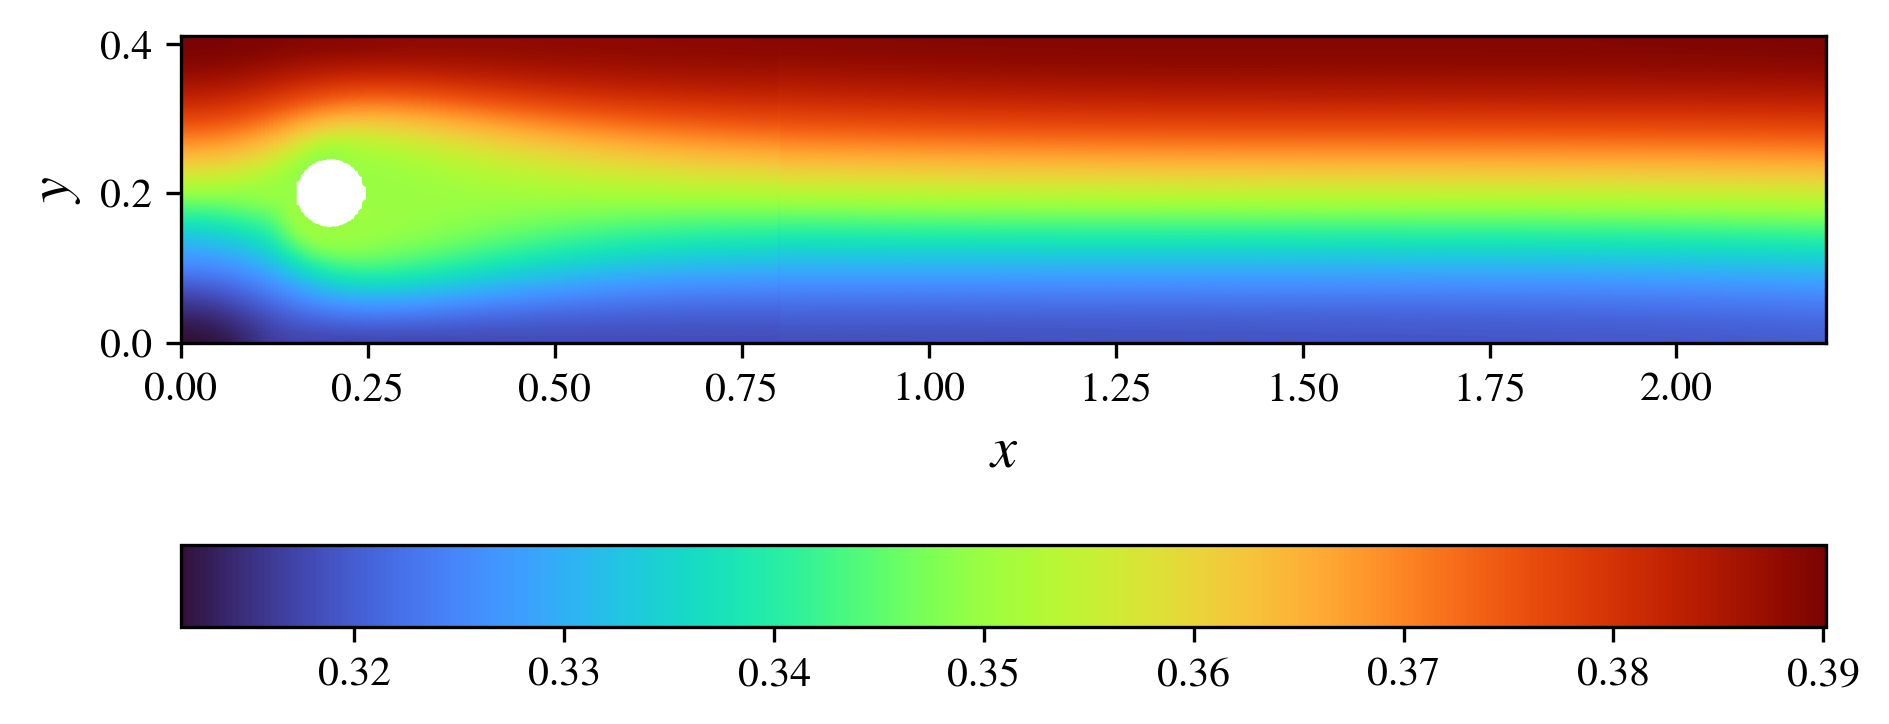
\includegraphics[width=\linewidth]{Project1XPINNs/figures/NavierStokes/TwoBoxDecomp/TB_10000_iter_right_emphasis/solution/streamfunc_two_box.png}
    \caption{Predicted streamfunction of the XPINN.}
    \label{fig:NS_XPINN_streamfunc}
\end{figure}

Along with the flow figures, the benchmark also provides drag and lift coefficients, as well as the pressure difference in front of and behind the cylinder. Our approximation of these results are seen in \autoref{table:NS_num}.

\begin{table}[h!]
\centering
\caption{Comparison with reference results.}
\begin{tabular}{r|c|c|c}
    \toprule
     & \hspace{5mm} Drag \hspace{5mm} & \hspace{5mm} Lift \hspace{5mm} & Pressure difference  \\
    \colrule
    DFG & 5.5795 &  0.0106 & 0.1175 \\
    PINN & 4.0687  &  -0.2542 & 0.0891 \\
    XPINN & 2.7482 & -0.3368 & 0.0557 \\
    \botrule
\end{tabular}
\label{table:NS_num}
\end{table}

\vfill\null



\label{sec:compexp}

\section{Conclusion}
% Discussion
Extended Physics-Informed Neural Networks represent an interesting development within machine learning.
Computational models have a tendency to adapt themselves to the constraint placed upon them by the computer architecture available at the time, from early CPU limitations to later memory constraints.
Currently, the best performing models are trained in large data centers, on huge datasets.
Improvements largely stem from the ability to train more complex models longer on more data, however we are seeing the early stages of being limited by environmental factors.

Large Language Models (LLMs), such as LLaMa \cite{touvron2023llama}, contain billions of parameters.
Recent work has explored 1.58bit models \cite{ma2024era}, where each weight $W_{ij}$ is constrained to be in $\{-1, 0, 1\}$, in order to reduce the size of the models.
Using simpler weights has the potential benefit of reducing the energy usage associated with training the models.
This more nuanced approach exemplifies the direction the field of machine learning seems to be moving, wherein models are specialized based on the problem at hand, rather than being brute force approximators.

% Conclusion
Based on our findings XPINNs do not seem to be the final advancement in the development of PINNs.
The constraints arising from diminished data availability, coupled with the emergence of interface losses, do not seem to be effectively counterbalanced by the solutions we were able to produce.
Augmented Physics-Informed Neural Networks (APINNs), introduced in \textcite{Hu_2023}, act as a natural evolution of XPINNs.
With APINNs, gating functions serve as the equivalent of the domain decomposition presented in this paper.
Using this methodology, each sub-PINN has access to all of the training data, and there are no hard boundaries introduced.

This is not to say that XPINNs are without merit, however we believe that further work should rather be placed on APINNs.
Another avenue for exploration is within the chosen optimizer.
Methods such as Energy Natural Gradient Descent \cite{müller2023achieving} have performed well in conjunction with PINNs, while learning rate free algorithms based on coin-betting ideas \cite{sharrock2023learning} perform remarkably well without the necessity of tuning the learning rate.
\label{sec:conclusion}

\bibliography{Project1XPINNs/References} % add references to this file

\appendix
\section{Source code}
The code is available at \url{https://github.com/augustfe/FYS5429}, along with a number of figures left out of this paper.

\end{document}
